% Options for packages loaded elsewhere
\PassOptionsToPackage{unicode}{hyperref}
\PassOptionsToPackage{hyphens}{url}
\documentclass[
]{article}
\usepackage{xcolor}
\usepackage[margin=1in]{geometry}
\usepackage{amsmath,amssymb}
\setcounter{secnumdepth}{5}
\usepackage{iftex}
\ifPDFTeX
  \usepackage[T1]{fontenc}
  \usepackage[utf8]{inputenc}
  \usepackage{textcomp} % provide euro and other symbols
\else % if luatex or xetex
  \usepackage{unicode-math} % this also loads fontspec
  \defaultfontfeatures{Scale=MatchLowercase}
  \defaultfontfeatures[\rmfamily]{Ligatures=TeX,Scale=1}
\fi
\usepackage{lmodern}
\ifPDFTeX\else
  % xetex/luatex font selection
\fi
% Use upquote if available, for straight quotes in verbatim environments
\IfFileExists{upquote.sty}{\usepackage{upquote}}{}
\IfFileExists{microtype.sty}{% use microtype if available
  \usepackage[]{microtype}
  \UseMicrotypeSet[protrusion]{basicmath} % disable protrusion for tt fonts
}{}
\makeatletter
\@ifundefined{KOMAClassName}{% if non-KOMA class
  \IfFileExists{parskip.sty}{%
    \usepackage{parskip}
  }{% else
    \setlength{\parindent}{0pt}
    \setlength{\parskip}{6pt plus 2pt minus 1pt}}
}{% if KOMA class
  \KOMAoptions{parskip=half}}
\makeatother
\usepackage{color}
\usepackage{fancyvrb}
\newcommand{\VerbBar}{|}
\newcommand{\VERB}{\Verb[commandchars=\\\{\}]}
\DefineVerbatimEnvironment{Highlighting}{Verbatim}{commandchars=\\\{\}}
% Add ',fontsize=\small' for more characters per line
\usepackage{framed}
\definecolor{shadecolor}{RGB}{248,248,248}
\newenvironment{Shaded}{\begin{snugshade}}{\end{snugshade}}
\newcommand{\AlertTok}[1]{\textcolor[rgb]{0.94,0.16,0.16}{#1}}
\newcommand{\AnnotationTok}[1]{\textcolor[rgb]{0.56,0.35,0.01}{\textbf{\textit{#1}}}}
\newcommand{\AttributeTok}[1]{\textcolor[rgb]{0.13,0.29,0.53}{#1}}
\newcommand{\BaseNTok}[1]{\textcolor[rgb]{0.00,0.00,0.81}{#1}}
\newcommand{\BuiltInTok}[1]{#1}
\newcommand{\CharTok}[1]{\textcolor[rgb]{0.31,0.60,0.02}{#1}}
\newcommand{\CommentTok}[1]{\textcolor[rgb]{0.56,0.35,0.01}{\textit{#1}}}
\newcommand{\CommentVarTok}[1]{\textcolor[rgb]{0.56,0.35,0.01}{\textbf{\textit{#1}}}}
\newcommand{\ConstantTok}[1]{\textcolor[rgb]{0.56,0.35,0.01}{#1}}
\newcommand{\ControlFlowTok}[1]{\textcolor[rgb]{0.13,0.29,0.53}{\textbf{#1}}}
\newcommand{\DataTypeTok}[1]{\textcolor[rgb]{0.13,0.29,0.53}{#1}}
\newcommand{\DecValTok}[1]{\textcolor[rgb]{0.00,0.00,0.81}{#1}}
\newcommand{\DocumentationTok}[1]{\textcolor[rgb]{0.56,0.35,0.01}{\textbf{\textit{#1}}}}
\newcommand{\ErrorTok}[1]{\textcolor[rgb]{0.64,0.00,0.00}{\textbf{#1}}}
\newcommand{\ExtensionTok}[1]{#1}
\newcommand{\FloatTok}[1]{\textcolor[rgb]{0.00,0.00,0.81}{#1}}
\newcommand{\FunctionTok}[1]{\textcolor[rgb]{0.13,0.29,0.53}{\textbf{#1}}}
\newcommand{\ImportTok}[1]{#1}
\newcommand{\InformationTok}[1]{\textcolor[rgb]{0.56,0.35,0.01}{\textbf{\textit{#1}}}}
\newcommand{\KeywordTok}[1]{\textcolor[rgb]{0.13,0.29,0.53}{\textbf{#1}}}
\newcommand{\NormalTok}[1]{#1}
\newcommand{\OperatorTok}[1]{\textcolor[rgb]{0.81,0.36,0.00}{\textbf{#1}}}
\newcommand{\OtherTok}[1]{\textcolor[rgb]{0.56,0.35,0.01}{#1}}
\newcommand{\PreprocessorTok}[1]{\textcolor[rgb]{0.56,0.35,0.01}{\textit{#1}}}
\newcommand{\RegionMarkerTok}[1]{#1}
\newcommand{\SpecialCharTok}[1]{\textcolor[rgb]{0.81,0.36,0.00}{\textbf{#1}}}
\newcommand{\SpecialStringTok}[1]{\textcolor[rgb]{0.31,0.60,0.02}{#1}}
\newcommand{\StringTok}[1]{\textcolor[rgb]{0.31,0.60,0.02}{#1}}
\newcommand{\VariableTok}[1]{\textcolor[rgb]{0.00,0.00,0.00}{#1}}
\newcommand{\VerbatimStringTok}[1]{\textcolor[rgb]{0.31,0.60,0.02}{#1}}
\newcommand{\WarningTok}[1]{\textcolor[rgb]{0.56,0.35,0.01}{\textbf{\textit{#1}}}}
\usepackage{longtable,booktabs,array}
\newcounter{none} % for unnumbered tables
\usepackage{calc} % for calculating minipage widths
% Correct order of tables after \paragraph or \subparagraph
\usepackage{etoolbox}
\makeatletter
\patchcmd\longtable{\par}{\if@noskipsec\mbox{}\fi\par}{}{}
\makeatother
% Allow footnotes in longtable head/foot
\IfFileExists{footnotehyper.sty}{\usepackage{footnotehyper}}{\usepackage{footnote}}
\makesavenoteenv{longtable}
\usepackage{graphicx}
\makeatletter
\newsavebox\pandoc@box
\newcommand*\pandocbounded[1]{% scales image to fit in text height/width
  \sbox\pandoc@box{#1}%
  \Gscale@div\@tempa{\textheight}{\dimexpr\ht\pandoc@box+\dp\pandoc@box\relax}%
  \Gscale@div\@tempb{\linewidth}{\wd\pandoc@box}%
  \ifdim\@tempb\p@<\@tempa\p@\let\@tempa\@tempb\fi% select the smaller of both
  \ifdim\@tempa\p@<\p@\scalebox{\@tempa}{\usebox\pandoc@box}%
  \else\usebox{\pandoc@box}%
  \fi%
}
% Set default figure placement to htbp
\def\fps@figure{htbp}
\makeatother
\setlength{\emergencystretch}{3em} % prevent overfull lines
\providecommand{\tightlist}{%
  \setlength{\itemsep}{0pt}\setlength{\parskip}{0pt}}
\usepackage{bookmark}
\IfFileExists{xurl.sty}{\usepackage{xurl}}{} % add URL line breaks if available
\urlstyle{same}
\hypersetup{
  pdftitle={Statistical Analysis of Rainfall Variability and Regional Monsoon Patterns in India},
  pdfauthor={B.Tech Probability and Statistics Course Project},
  hidelinks,
  pdfcreator={LaTeX via pandoc}}

\title{Statistical Analysis of Rainfall Variability and Regional Monsoon
Patterns in India}
\usepackage{etoolbox}
\makeatletter
\providecommand{\subtitle}[1]{% add subtitle to \maketitle
  \apptocmd{\@title}{\par {\large #1 \par}}{}{}
}
\makeatother
\subtitle{An undergraduate Probability and Statistics project using
India Meteorological Department rainfall records}
\author{B.Tech Probability and Statistics Course Project}
\date{October 2026}

\begin{document}
\maketitle

{
\setcounter{tocdepth}{3}
\tableofcontents
}
\newpage

\section{Title page}\label{title-page}

\textbf{Project title.} Statistical Analysis of Rainfall Variability and
Regional Monsoon Patterns in India

\textbf{Course.} Probability and Statistics (undergraduate / B.Tech)

\textbf{Software.} R 4.6.1 and RStudio; analysis scripts in
\texttt{R\_code/}

\textbf{Data.} India Meteorological Department (IMD) area-weighted
all-India rainfall, 1901--2015, and IMD meteorological subdivision
rainfall, 1901--2017

\textbf{Units.} Millimetres (mm) throughout

\textbf{Declaration.} All numerical results in this report are taken
from the project's saved R outputs. No external rainfall datasets were
added, and no values were invented. Student name, roll number and
institution should be written here before submission.

\newpage

\section{Abstract}\label{abstract}

This project studies rainfall variability and monsoon patterns over
India using two official India Meteorological Department (IMD) series:
an all-India \textbf{area-weighted} monthly-to-annual record for
1901--2015 (\(n = 115\) complete years) and a panel of \textbf{36
meteorological subdivisions} for 1901--2017. After a documented quality
audit, the original CSV files were left unchanged and analysis copies
were used. All-India mean annual rainfall is 1182.03 mm (median 1190.50
mm; SD 110.69 mm; CV 9.36\%). About three-quarters of that mean (75.3\%)
falls in June--September. Historical relative frequencies, with an
IMD-style 90\%/110\% rule applied to \emph{this} series mean, classify
21.7\% of years as deficient monsoon, 64.3\% as normal and 13.9\% as
excess. All-India annual totals are close to both a normal and a gamma
model (Shapiro--Wilk \(p =\) 0.8014; bootstrap Kolmogorov--Smirnov
\(p =\) 0.3725 for gamma); an exponential model is incompatible with the
data. A 95\% \(t\) interval for the all-India mean annual total is
1161.59 to 1202.48 mm under an independent-years approximation. Tests
confirm the expected climatic contrasts (southwest monsoon versus
post-monsoon; Kerala versus West Rajasthan) and do \textbf{not} detect a
statistically significant linear or Mann--Kendall trend in all-India
annual rainfall over 1901--2015. Serial correlation at lag 2 and the
fact that years are a single climate path, not a simple random sample,
limit causal language. Correlation is not treated as causation, and this
analysis does not prove climate change.

\section{Introduction}\label{introduction}

Rainfall over India is concentrated in a few months, varies sharply from
the Western Ghats and north-east to the Thar Desert, and is the main
natural control on agriculture and water supply. Undergraduate
Probability and Statistics is well suited to this topic: the data are
continuous millimetre measurements, they come in months, seasons and
years, and they exist both as a national series and as regional series.

The scientific aim is modest and honest. The project \textbf{describes}
the 1901--2015 all-India record and \textbf{compares} selected IMD
subdivisions. It estimates means and proportions with confidence
intervals, tests clearly stated hypotheses, fits simple probability
models, and looks for monotonic association with time. It does not
reconstruct daily storms, does not downscale climate models, and does
not attribute rainfall change to greenhouse gases.

Two government files already in \texttt{data/} are used and never
replaced. Scripts \texttt{R\_code/01}--\texttt{09} produce the tables in
\texttt{results/tables/} and the figures in \texttt{graphs/}. This
report cites those artefacts.

\section{Problem statement}\label{problem-statement}

Decision makers often quote a single ``average Indian rainfall'' and a
simple wet/dry story. The data are richer and more awkward than that
slogan:

\begin{itemize}
\tightlist
\item
  The national series is \textbf{area-weighted}. It is not the
  unweighted mean of 36 subdivisions.
\item
  Many subdivision years are missing some months. Annual totals are then
  undefined unless missing months are ignored, which would be incorrect.
\item
  Rainfall is bounded below by zero, often skewed in dry months, and
  ordered in time, so textbook normal and independent-sample assumptions
  need checking.
\item
  Seasonal totals that add up to the annual total must not be correlated
  with the annual total as if they were independent causes.
\end{itemize}

The problem is therefore to apply a wide, but \emph{justified}, set of
probability and statistics tools to these two series, to report what the
numbers support, and to state clearly what they do not support.

\section{Aim and objectives}\label{aim-and-objectives}

\textbf{Aim.} To quantify rainfall variability and regional monsoon
contrasts in India from official IMD records using standard methods of
Probability and Statistics, with fully reproducible R code.

\textbf{Objectives.}

\begin{enumerate}
\def\labelenumi{\arabic{enumi}.}
\tightlist
\item
  Audit and clean the two source files without fabricating rainfall.
\item
  Describe monthly, seasonal, annual and regional rainfall with
  appropriate summaries.
\item
  Compute empirical probabilities with explicit thresholds and
  denominators.
\item
  Assess normal, gamma and exponential models, including zeros where
  they occur.
\item
  Demonstrate sampling variability, the Central Limit Theorem, and
  confidence intervals.
\item
  Test pre-registered hypotheses at \(\alpha = 0.05\).
\item
  Study association among \emph{different} seasons, not part--whole
  pairs.
\item
  Fit simple and multiple linear regressions only where a question
  exists.
\item
  Compare regions with ANOVA or a robust alternative after checking
  variances.
\item
  Describe time series behaviour and test for monotonic trend without
  claiming attribution.
\end{enumerate}

\section{Research questions}\label{research-questions}

\begin{enumerate}
\def\labelenumi{\arabic{enumi}.}
\tightlist
\item
  What are the location, spread and shape of all-India monthly, seasonal
  and annual rainfall in 1901--2015?
\item
  How often, in this record, was the southwest monsoon deficient, normal
  or excess under a stated 90\%/110\% rule?
\item
  Is a normal, gamma or exponential law a reasonable model for all-India
  annual rainfall?
\item
  How precise is the estimated all-India mean, and how does interval
  width change with confidence level?
\item
  Does the all-India mean differ from a 1180 mm textbook benchmark?
\item
  Do Kerala and West Rajasthan differ in mean annual rainfall?
\item
  Within the same year, does June--September rainfall differ from
  October--December rainfall?
\item
  Are the four IMD seasons equally likely to be the wettest season?
\item
  How strongly are winter and monsoon rainfall associated?
\item
  Is there a statistically detectable linear or monotonic trend in
  all-India annual rainfall over 1901--2015?
\item
  How do mean rainfall and relative variability differ among IMD
  subdivisions?
\end{enumerate}

\section{Dataset descriptions and official
sources}\label{dataset-descriptions-and-official-sources}

\subsection{Provenance}\label{provenance}

Both files are rainfall series of the \textbf{India Meteorological
Department (IMD), Ministry of Earth Sciences, Government of India}. They
were supplied as CSV files in \texttt{data/} and were not downloaded
from third-party contest sites for this project.

{\def\LTcaptype{none} % do not increment counter
\begin{longtable}[]{@{}
  >{\raggedright\arraybackslash}p{(\linewidth - 6\tabcolsep) * \real{0.2500}}
  >{\raggedright\arraybackslash}p{(\linewidth - 6\tabcolsep) * \real{0.2500}}
  >{\raggedright\arraybackslash}p{(\linewidth - 6\tabcolsep) * \real{0.2500}}
  >{\raggedright\arraybackslash}p{(\linewidth - 6\tabcolsep) * \real{0.2500}}@{}}
\toprule\noalign{}
\begin{minipage}[b]{\linewidth}\raggedright
File
\end{minipage} & \begin{minipage}[b]{\linewidth}\raggedright
Spatial support
\end{minipage} & \begin{minipage}[b]{\linewidth}\raggedright
Time span in file
\end{minipage} & \begin{minipage}[b]{\linewidth}\raggedright
Role in this project
\end{minipage} \\
\midrule\noalign{}
\endhead
\bottomrule\noalign{}
\endlastfoot
\texttt{data/rainfall\_area-wt\_India\_1901-2015.csv} & One all-India
area-weighted series (\texttt{REGION\ =\ INDIA}) & 1901--2015 & National
climatology, distributions, inference, trend \\
\texttt{data/Sub\_Division\_IMD\_2017.csv} & 36 IMD meteorological
subdivisions & 1901--2017 (unbalanced) & Regional means, CV, ANOVA,
selected regional trends \\
\end{longtable}
}

\subsection{Schema actually used}\label{schema-actually-used}

The national file has columns \texttt{REGION}, \texttt{YEAR}, months
\texttt{JAN}--\texttt{DEC}, \texttt{ANNUAL}, and seasons
\texttt{Jan-Feb}, \texttt{Mar-May}, \texttt{Jun-Sep}, \texttt{Oct-Dec}.

The subdivision file has \texttt{SUBDIVISION}, \texttt{YEAR}, months
\texttt{JAN}--\texttt{DEC}, \texttt{ANNUAL}, and seasons \texttt{JF},
\texttt{MAM}, \texttt{JJAS}, \texttt{OND}.

Season groups follow the standard IMD calendar: winter
(January--February), pre-monsoon (March--May), southwest monsoon
(June--September), post-monsoon (October--December). Units are
millimetres. A recorded \textbf{zero is a dry month}, not a missing
value. The token \texttt{NA} in the subdivision file is a true missing
report.

\subsection{Geographical and temporal
scope}\label{geographical-and-temporal-scope}

The national series has 115 rows, one per year, with no internal year
gap. The subdivision file has 4188 rows. Arunachal Pradesh starts in
1916. Internal missing years include Andaman \& Nicobar Islands (1909,
1943--1945, 1948), Arunachal Pradesh (1954--1956) and Lakshadweep
(1918). Joint national--regional work uses 1901--2015. The two extra
subdivision years 2016--2017 are not mixed into national trend tests.

\section{Data cleaning and
preprocessing}\label{data-cleaning-and-preprocessing}

Cleaning is implemented in \texttt{R\_code/01\_data\_inspection.R} and
\texttt{R\_code/02\_data\_cleaning.R}. Original files in \texttt{data/}
were never overwritten. Analysis copies live in
\texttt{results/cleaned\_data/}.

Table 1 records every transformation and the number of affected
observations (from \texttt{results/tables/cleaning\_log.csv}).

\begin{longtable}[]{@{}
  >{\raggedleft\arraybackslash}p{(\linewidth - 8\tabcolsep) * \real{0.0213}}
  >{\raggedright\arraybackslash}p{(\linewidth - 8\tabcolsep) * \real{0.0979}}
  >{\raggedright\arraybackslash}p{(\linewidth - 8\tabcolsep) * \real{0.1745}}
  >{\raggedleft\arraybackslash}p{(\linewidth - 8\tabcolsep) * \real{0.0468}}
  >{\raggedright\arraybackslash}p{(\linewidth - 8\tabcolsep) * \real{0.6596}}@{}}
\caption{Table 1. Cleaning log (analysis copies only; originals
untouched).}\tabularnewline
\toprule\noalign{}
\begin{minipage}[b]{\linewidth}\raggedleft
Step
\end{minipage} & \begin{minipage}[b]{\linewidth}\raggedright
Dataset
\end{minipage} & \begin{minipage}[b]{\linewidth}\raggedright
Action
\end{minipage} & \begin{minipage}[b]{\linewidth}\raggedleft
n affected
\end{minipage} & \begin{minipage}[b]{\linewidth}\raggedright
Justification
\end{minipage} \\
\midrule\noalign{}
\endfirsthead
\toprule\noalign{}
\begin{minipage}[b]{\linewidth}\raggedleft
Step
\end{minipage} & \begin{minipage}[b]{\linewidth}\raggedright
Dataset
\end{minipage} & \begin{minipage}[b]{\linewidth}\raggedright
Action
\end{minipage} & \begin{minipage}[b]{\linewidth}\raggedleft
n affected
\end{minipage} & \begin{minipage}[b]{\linewidth}\raggedright
Justification
\end{minipage} \\
\midrule\noalign{}
\endhead
\bottomrule\noalign{}
\endlastfoot
1 & national\_area\_weighted & import & 115 & Read original CSV with
explicit NA strings; originals not modified. \\
2 & national\_area\_weighted & trim\_REGION & 0 & Remove
leading/trailing whitespace from region labels. \\
3 & national\_area\_weighted & YEAR\_to\_integer & 0 & Calendar year is
a discrete index, not a continuous measurement. \\
4 & national\_area\_weighted & rainfall\_to\_numeric & 0 & Rainfall is a
continuous millimetre measurement; coercion failures would become NA
(none expected). \\
5 & national\_area\_weighted & negative\_rainfall\_screen & 0 & Negative
millimetres are physically impossible; none are deleted because none
were found, or they would be flagged not dropped. \\
6 & national\_area\_weighted & duplicate\_investigation & 0 & Exact row
duplicates and REGION-YEAR duplicates were counted. No rows removed
because none were found. \\
7 & national\_area\_weighted & consistency\_flags & 0 & Source
seasonal/annual totals were retained. Differences \textgreater{} 1 mm
versus the sum of constituent months are flagged, not overwritten. \\
8 & national\_area\_weighted & annual\_reconstruct\_if\_source\_NA & 0 &
Not imputation of unobserved rain: ANNUAL is a total of observed months.
Filled only when all 12 months exist and source ANNUAL is NA. \\
9 & national\_area\_weighted & outlier\_flag\_iqr\_k3 & 2 & Extreme
rainfall years are scientifically informative (floods/droughts). Flagged
with a conservative 3xIQR rule; no rows deleted. \\
10 & national\_area\_weighted & write\_cleaned\_copy & 115 & Analysis
copy written; original data/ CSV untouched. \\
11 & imd\_subdivision & import & 4188 & Read original CSV with explicit
NA strings; originals not modified. \\
12 & imd\_subdivision & standardise\_SUBDIVISION\_whitespace & 0 & Trim
and collapse repeated whitespace. Historical IMD names (Orissa,
Matathwada, Rayalseema) are retained so records stay matchable to the
source. \\
13 & imd\_subdivision & YEAR\_to\_integer & 0 & Calendar year is a
discrete index. \\
14 & imd\_subdivision & rainfall\_to\_numeric & 0 & Rainfall coerced to
numeric millimetres. Source `NA' tokens already mapped to R NA on
import. \\
15 & imd\_subdivision & retain\_zeros\_and\_missing & 70 & Zero
millimetres remain as dry months. NA remains missing. Incomplete rows
were not deleted. \\
16 & imd\_subdivision & negative\_rainfall\_screen & 0 & Negative
rainfall would be flagged, not deleted. \\
17 & imd\_subdivision & duplicate\_investigation & 0 & No
SUBDIVISION-YEAR duplicates. No rows removed. \\
18 & imd\_subdivision & consistency\_flags & 0 & Source derived totals
retained. Inconsistencies \textgreater{} 1 mm versus complete month sums
are flagged, not overwritten. \\
19 & imd\_subdivision & reconstruct\_derived\_totals\_if\_source\_NA & 0
& Where IMD omitted ANNUAL/JF/MAM/JJAS/OND but all constituent months
are observed, the analysis column is the month sum. This does not invent
monthly rain. \\
20 & imd\_subdivision & outlier\_flag\_iqr\_k3\_by\_subdivision\_month &
887 & Outliers flagged within each subdivision and month using 3xIQR.
Extreme monsoon totals are retained. \\
21 & imd\_subdivision & retain\_unbalanced\_panel & 9 & Internal missing
years (e.g.~a subdivision with 1908 then 1910) are left as absent rows.
No years were invented. \\
22 & imd\_subdivision & write\_cleaned\_copy & 4188 & Analysis copy
written; original data/ CSV untouched. \\
\end{longtable}

\textbf{Decisions that matter for later inference.}

\begin{itemize}
\tightlist
\item
  \textbf{Missing months.} Seventy monthly cells in the subdivision file
  are \texttt{NA}. Incomplete rows were \textbf{kept}. Annual and
  monsoon analyses of subdivisions use years with all 12 months observed
  (\texttt{months\_complete}).
\item
  \textbf{Zeros.} 3720 monthly zeros were retained as genuine dry
  months.
\item
  \textbf{No imputation.} Where a source annual or seasonal total was
  missing, reconstruction from months was allowed only if every
  constituent month was present. That case never occurred
  (\texttt{ANNUAL\_filled\ =\ 0}), because every missing annual already
  had a missing month.
\item
  \textbf{Duplicates.} None in either file.
\item
  \textbf{Consistency.} Source seasonal and annual totals agree with
  month sums within rounding (maximum absolute difference 0.3 mm
  nationally and 0.4 mm for subdivision annual totals). Nothing was
  overwritten.
\item
  \textbf{Outliers.} Conservative \(3\times\)IQR flags were stored. Two
  national rows and 887 subdivision rows had at least one flagged month.
  \textbf{No extreme year was deleted}; wet and dry extremes are part of
  the climate.
\item
  \textbf{Labels.} Historical IMD names (Orissa, Matathwada, Rayalseema)
  were kept after trimming whitespace.
\end{itemize}

\section{Statistical methodology}\label{statistical-methodology}

Notation: \(X_1,\ldots,X_n\) are rainfall values in millimetres for a
stated series; \(\bar x\) is the sample mean; \(s\) is the sample
standard deviation with divisor \(n-1\); \(\alpha = 0.05\) unless
stated.

\textbf{Mean, variance, SD and CV.} \[
\bar x = \frac{1}{n}\sum_{i=1}^n x_i,\qquad
s^2 = \frac{1}{n-1}\sum_{i=1}^n (x_i-\bar x)^2,\qquad
\mathrm{CV} = 100\cdot\frac{s}{\bar x}.
\] The CV compares relative variability of a wet coast and a dry desert.

\textbf{Standard error of the mean} (independent observations):
\(\mathrm{SE}(\bar x)=s/\sqrt{n}\).

\textbf{Student \(t\) interval} for a mean: \[
\bar x \pm t_{n-1,1-\alpha/2}\,\frac{s}{\sqrt{n}}.
\]

\textbf{Wald interval} for a proportion \(\hat p = x/n\): \[
\hat p \pm z_{1-\alpha/2}\sqrt{\hat p(1-\hat p)/n}.
\]

\textbf{Pearson correlation} (for linear association, not causation): \[
r = \frac{\sum (x_i-\bar x)(y_i-\bar y)}{\sqrt{\sum(x_i-\bar x)^2\sum(y_i-\bar y)^2}}.
\]

\textbf{Simple linear regression.}
\(Y_i = \beta_0 + \beta_1 t_i + \varepsilon_i\) with year \(t_i\).
Ordinary least squares is used as a \emph{descriptive} line. Residual
plots, Shapiro--Wilk on residuals, a screen of \(e_i^2\) against fitted
values, Cook's distance and the Durbin--Watson statistic
\(d=\sum(\hat e_i-\hat e_{i-1})^2/\sum\hat e_i^2\) are reported. If
residuals are serially correlated, OLS \(p\)-values are treated as
approximate.

\textbf{Welch two-sample \(t\)} is used when two \emph{places} are
compared and variances differ. \textbf{Paired \(t\)} is used when two
seasons belong to the \emph{same year}. Independent-sample tests are not
applied to paired seasons.

\textbf{ANOVA.} Classical one-way ANOVA assumes independent groups,
similar variances and approximate normality. Fligner--Killeen tests
variances. If they differ, \textbf{Welch ANOVA} and Bonferroni pairwise
Welch tests are preferred; Kruskal--Wallis is reported as a rank
alternative.

\textbf{Distributions.} Gamma (positive, possibly skewed) is fitted by
maximum likelihood. Exponential (gamma with shape 1, and
\(\mathrm{SD}=\mathrm{mean}\)) is fitted only as a poor reference. The
ordinary one-sample Kolmogorov--Smirnov \(p\)-value is \textbf{not} used
when parameters are estimated from the same sample (Lilliefors problem).
A parametric bootstrap with \(B=400\) and seed 19012015 re-estimates
parameters in each replicate.

\textbf{Trend.} Mann--Kendall tests \(H_0\): no monotonic trend, using
\[
S=\sum_{i<j}\mathrm{sign}(x_j-x_i),
\] with a normal approximation for \(Z\) after a tie correction. Sen's
slope is the median of pairwise slopes \((x_j-x_i)/(t_j-t_i)\). These
tests describe association with time in 1901--2015; they are not
attribution.

\textbf{Software.} Base R 4.6.1 only for analysis (\texttt{stats},
\texttt{graphics}, \texttt{grDevices}). Random seed for simulations:
19012015.

\section{Descriptive statistics}\label{descriptive-statistics}

All-India results use 115 complete years, 1901--2015. Table 2 summarises
seasons and the year.

\begin{longtable}[]{@{}
  >{\raggedright\arraybackslash}p{(\linewidth - 18\tabcolsep) * \real{0.2708}}
  >{\raggedleft\arraybackslash}p{(\linewidth - 18\tabcolsep) * \real{0.0417}}
  >{\raggedleft\arraybackslash}p{(\linewidth - 18\tabcolsep) * \real{0.0833}}
  >{\raggedleft\arraybackslash}p{(\linewidth - 18\tabcolsep) * \real{0.0729}}
  >{\raggedleft\arraybackslash}p{(\linewidth - 18\tabcolsep) * \real{0.0729}}
  >{\raggedleft\arraybackslash}p{(\linewidth - 18\tabcolsep) * \real{0.0625}}
  >{\raggedleft\arraybackslash}p{(\linewidth - 18\tabcolsep) * \real{0.0625}}
  >{\raggedleft\arraybackslash}p{(\linewidth - 18\tabcolsep) * \real{0.0729}}
  >{\raggedleft\arraybackslash}p{(\linewidth - 18\tabcolsep) * \real{0.0938}}
  >{\raggedleft\arraybackslash}p{(\linewidth - 18\tabcolsep) * \real{0.1667}}@{}}
\caption{Table 2. All-India seasonal and annual rainfall (mm),
1901--2015.}\tabularnewline
\toprule\noalign{}
\begin{minipage}[b]{\linewidth}\raggedright
Series
\end{minipage} & \begin{minipage}[b]{\linewidth}\raggedleft
n
\end{minipage} & \begin{minipage}[b]{\linewidth}\raggedleft
Mean
\end{minipage} & \begin{minipage}[b]{\linewidth}\raggedleft
Median
\end{minipage} & \begin{minipage}[b]{\linewidth}\raggedleft
SD
\end{minipage} & \begin{minipage}[b]{\linewidth}\raggedleft
CV \%
\end{minipage} & \begin{minipage}[b]{\linewidth}\raggedleft
Min
\end{minipage} & \begin{minipage}[b]{\linewidth}\raggedleft
Max
\end{minipage} & \begin{minipage}[b]{\linewidth}\raggedleft
Skewness
\end{minipage} & \begin{minipage}[b]{\linewidth}\raggedleft
Excess kurtosis
\end{minipage} \\
\midrule\noalign{}
\endfirsthead
\toprule\noalign{}
\begin{minipage}[b]{\linewidth}\raggedright
Series
\end{minipage} & \begin{minipage}[b]{\linewidth}\raggedleft
n
\end{minipage} & \begin{minipage}[b]{\linewidth}\raggedleft
Mean
\end{minipage} & \begin{minipage}[b]{\linewidth}\raggedleft
Median
\end{minipage} & \begin{minipage}[b]{\linewidth}\raggedleft
SD
\end{minipage} & \begin{minipage}[b]{\linewidth}\raggedleft
CV \%
\end{minipage} & \begin{minipage}[b]{\linewidth}\raggedleft
Min
\end{minipage} & \begin{minipage}[b]{\linewidth}\raggedleft
Max
\end{minipage} & \begin{minipage}[b]{\linewidth}\raggedleft
Skewness
\end{minipage} & \begin{minipage}[b]{\linewidth}\raggedleft
Excess kurtosis
\end{minipage} \\
\midrule\noalign{}
\endhead
\bottomrule\noalign{}
\endlastfoot
annual & 115 & 1182.03 & 1190.5 & 110.69 & 9.36 & 920.8 & 1480.3 & 0.02
& -0.19 \\
Jan-Feb winter & 115 & 43.19 & 41.3 & 14.48 & 33.52 & 11.7 & 86.3 & 0.39
& 0.01 \\
Mar-May pre-monsoon & 115 & 128.69 & 125.1 & 22.90 & 17.79 & 84.5 &
209.7 & 0.74 & 0.80 \\
Jun-Sep southwest monsoon & 115 & 890.26 & 897.8 & 89.18 & 10.02 & 679.5
& 1094.5 & -0.29 & -0.43 \\
Oct-Dec post-monsoon & 115 & 119.88 & 116.2 & 32.47 & 27.08 & 52.7 &
207.5 & 0.38 & -0.23 \\
\end{longtable}

\textbf{What the measures say.} The mean annual total is 1182.03 mm and
the median is 1190.50 mm, so the centre is not being pulled by a few
catastrophic years. The range is 920.80 to 1480.30 mm. The SD of 110.69
mm and CV of 9.36\% show moderate year-to-year variation \emph{relative
to the mean}. Skewness 0.020 and excess kurtosis -0.193 are close to the
normal values 0 and 0: at the all-India annual scale, spatial averaging
has already removed much of the skewness seen in local daily rain. A
unique sample mode after rounding to 0.1 mm does not exist for annual
totals (continuous series with almost unique values).

June--September averages 890.26 mm, which is 75.3\% of the annual mean.
Winter averages only 43.19 mm. Relative variability is highest in winter
(CV 33.52\%) and post-monsoon (CV 27.08\%), and lowest in the monsoon
(CV 10.02\%).

\begin{figure}

{\centering 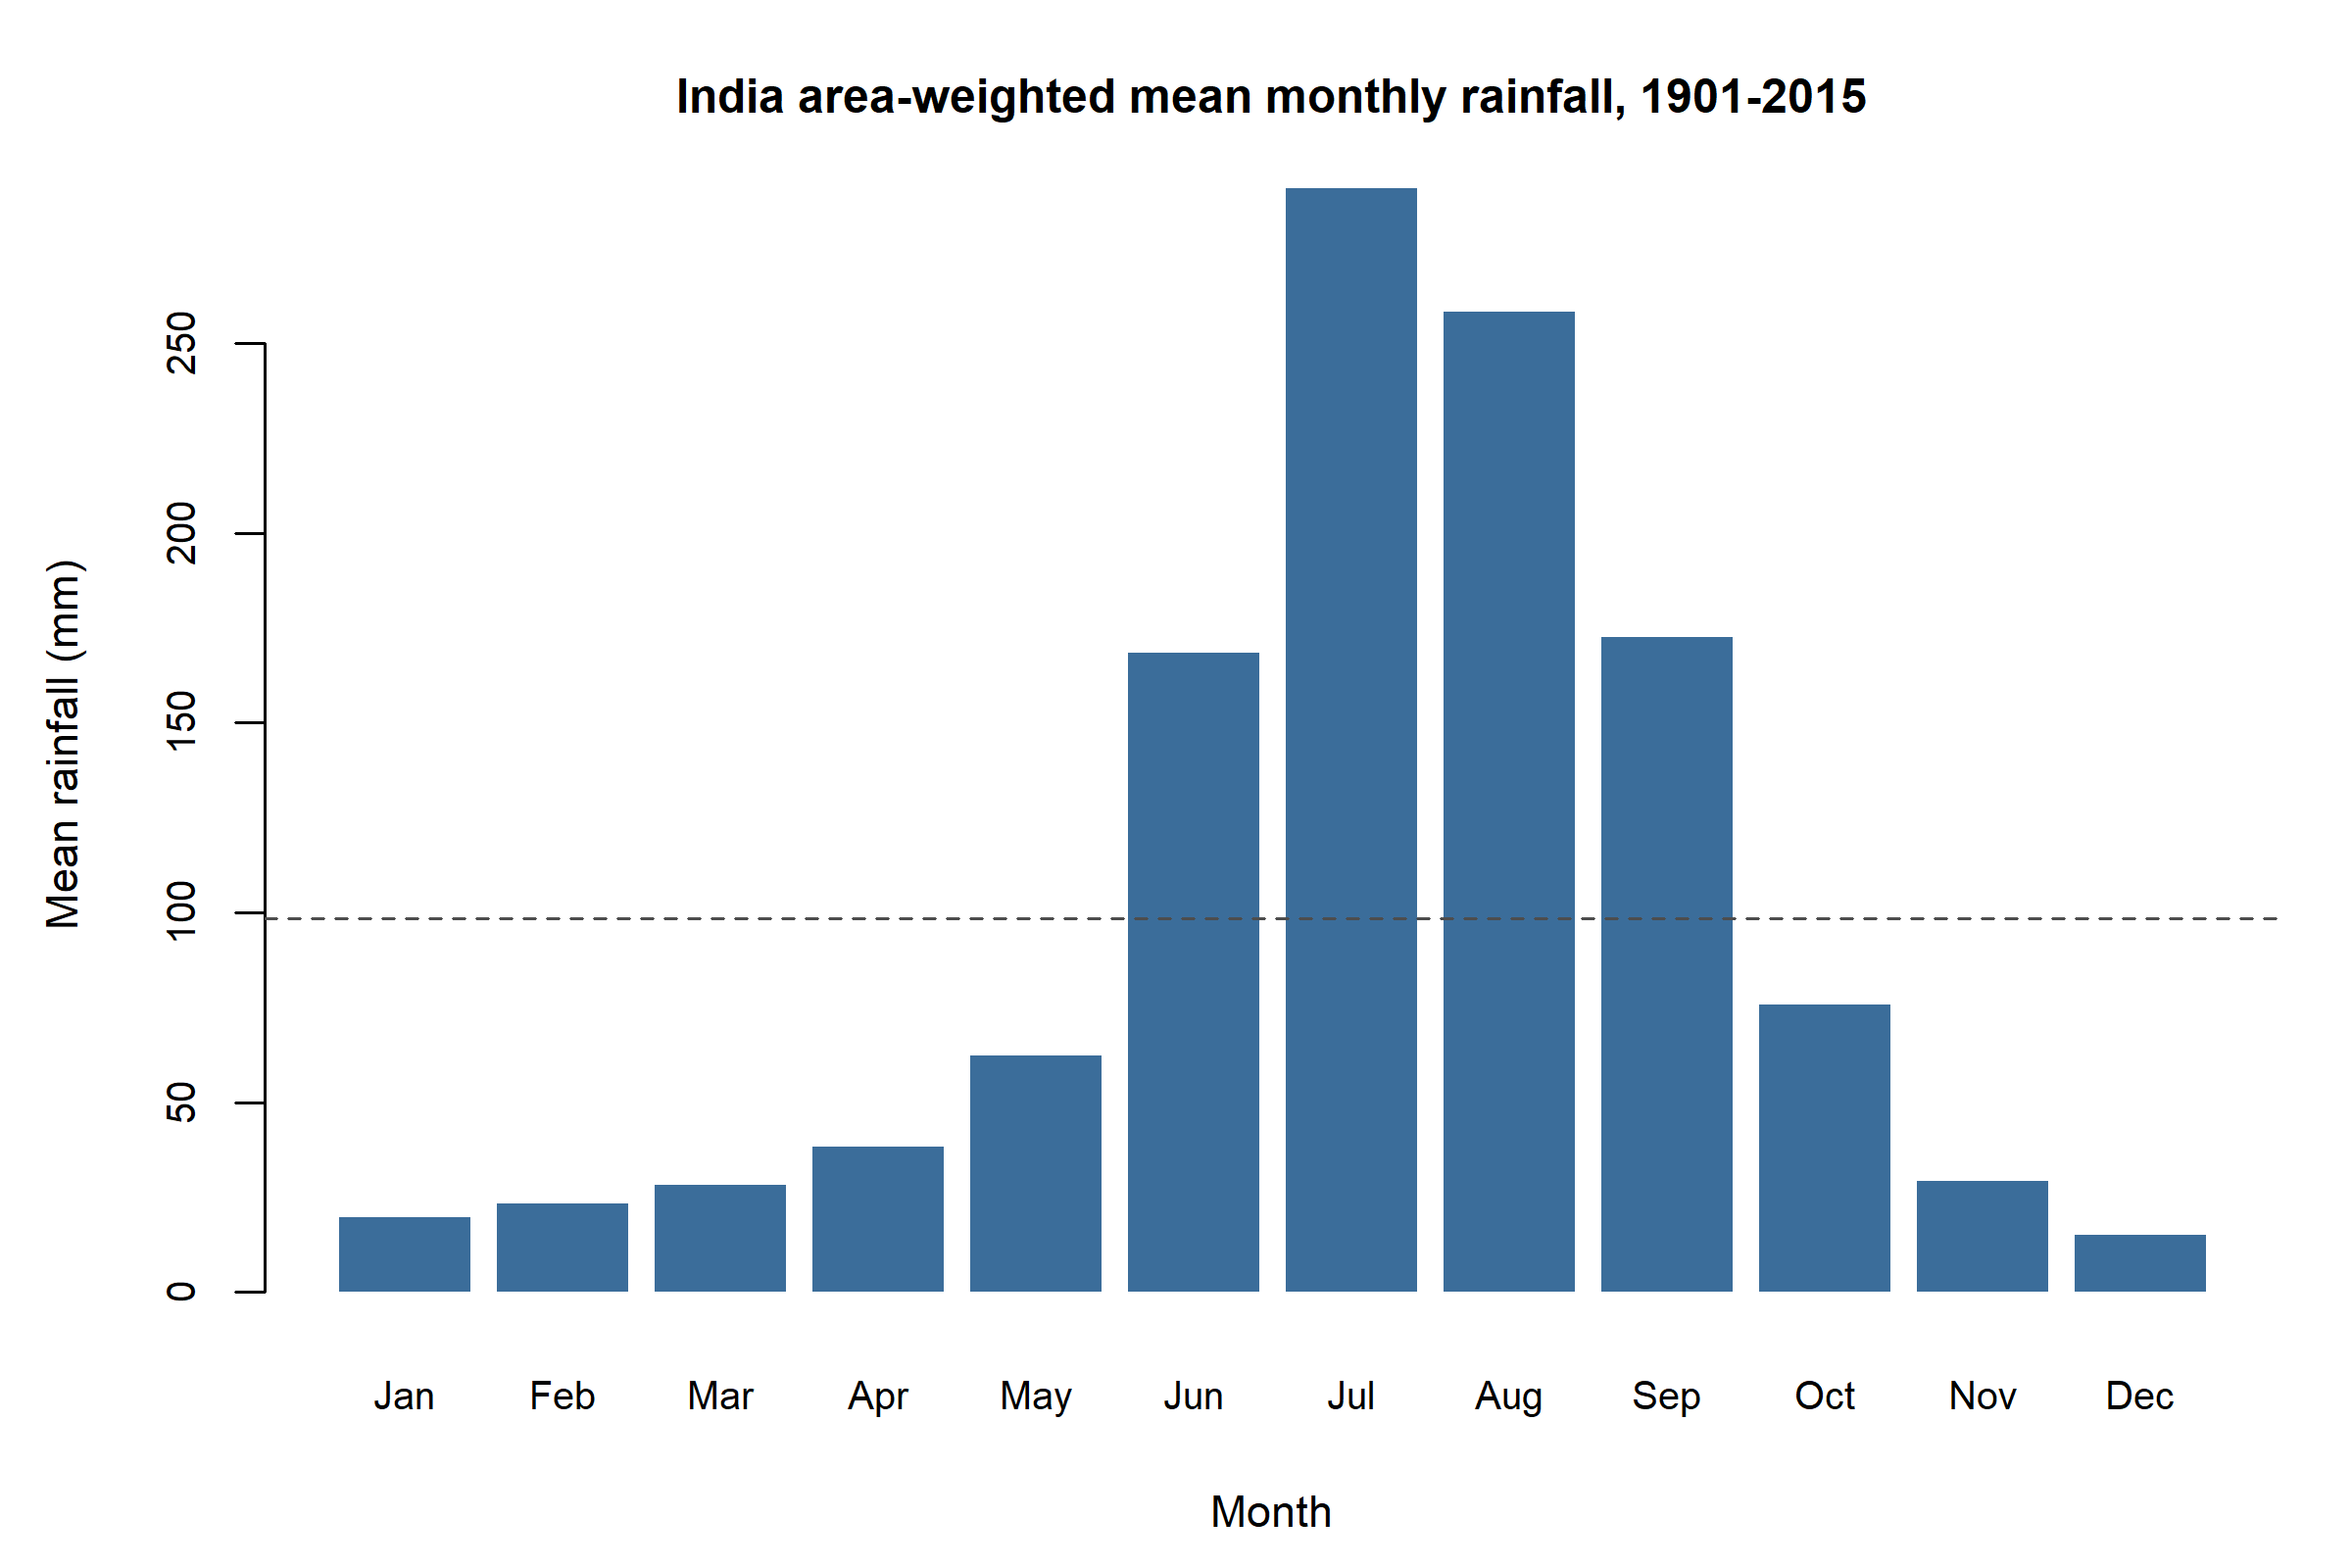
\includegraphics[width=0.92\linewidth]{../graphs/india_monthly_mean_rainfall} 

}

\caption{Figure 1. All-India area-weighted mean monthly rainfall (mm), 1901–2015.}\label{fig:fig-monthly-mean}
\end{figure}

Figure 1 and Table 3 show the annual cycle: July (291.02 mm) and August
(258.40 mm) dominate; December is driest (14.98 mm) with the largest CV
(58.67\%).

\begin{longtable}[]{@{}lrrrrrr@{}}
\caption{Table 3. All-India monthly rainfall (mm), 1901--2015, n =
115.}\tabularnewline
\toprule\noalign{}
Month & Mean & Median & SD & CV \% & Min & Max \\
\midrule\noalign{}
\endfirsthead
\toprule\noalign{}
Month & Mean & Median & SD & CV \% & Min & Max \\
\midrule\noalign{}
\endhead
\bottomrule\noalign{}
\endlastfoot
JAN & 19.76 & 17.8 & 9.99 & 50.57 & 2.7 & 58.5 \\
FEB & 23.43 & 22.5 & 11.51 & 49.13 & 2.7 & 53.8 \\
MAR & 28.25 & 25.5 & 12.29 & 43.48 & 7.2 & 63.3 \\
APR & 38.24 & 37.4 & 10.35 & 27.07 & 16.1 & 69.4 \\
MAY & 62.19 & 59.5 & 15.67 & 25.20 & 32.1 & 114.5 \\
JUN & 168.36 & 165.6 & 35.57 & 21.13 & 86.5 & 275.5 \\
JUL & 291.02 & 295.8 & 41.16 & 14.14 & 138.9 & 383.4 \\
AUG & 258.40 & 259.3 & 34.98 & 13.54 & 191.7 & 335.5 \\
SEP & 172.47 & 173.1 & 36.64 & 21.24 & 96.9 & 281.0 \\
OCT & 75.70 & 69.2 & 28.27 & 37.34 & 20.0 & 158.8 \\
NOV & 29.21 & 26.1 & 16.10 & 55.13 & 3.6 & 74.2 \\
DEC & 14.98 & 14.1 & 8.79 & 58.67 & 1.6 & 54.4 \\
\end{longtable}

\begin{figure}

{\centering 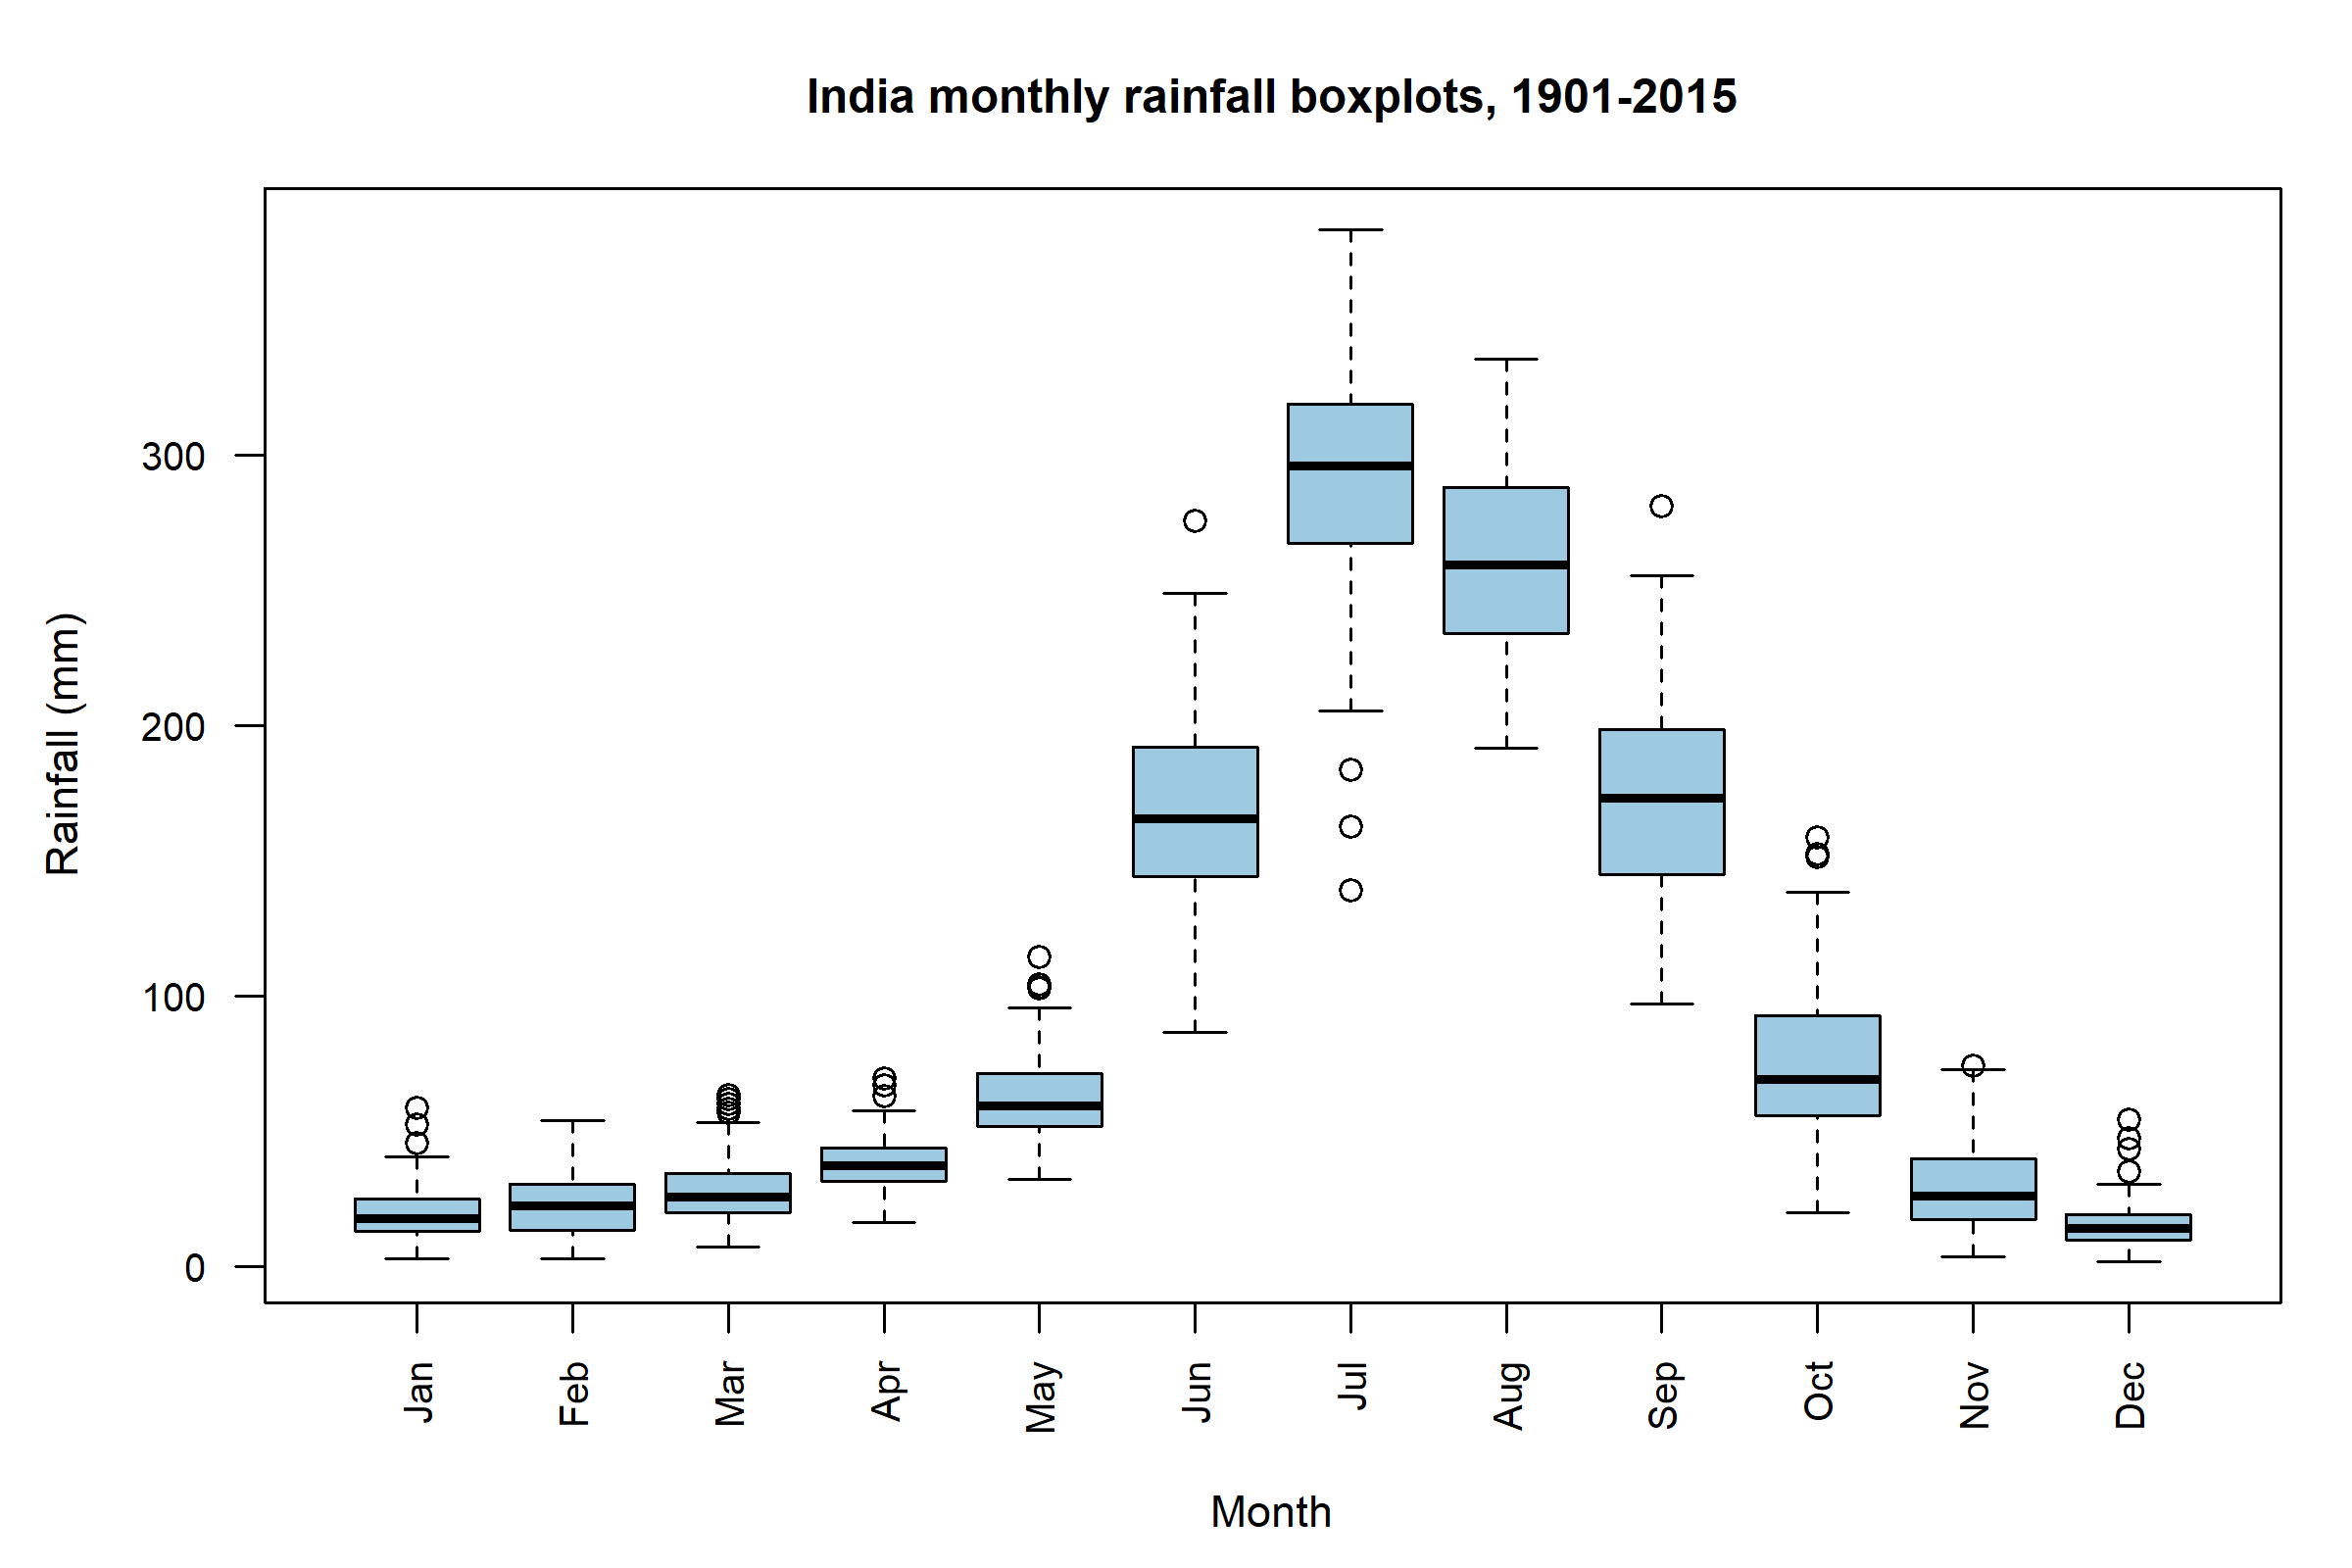
\includegraphics[width=0.92\linewidth]{../graphs/india_monthly_boxplots} 

}

\caption{Figure 2. All-India monthly rainfall boxplots (mm), 1901–2015.}\label{fig:fig-month-box}
\end{figure}

\begin{figure}

{\centering 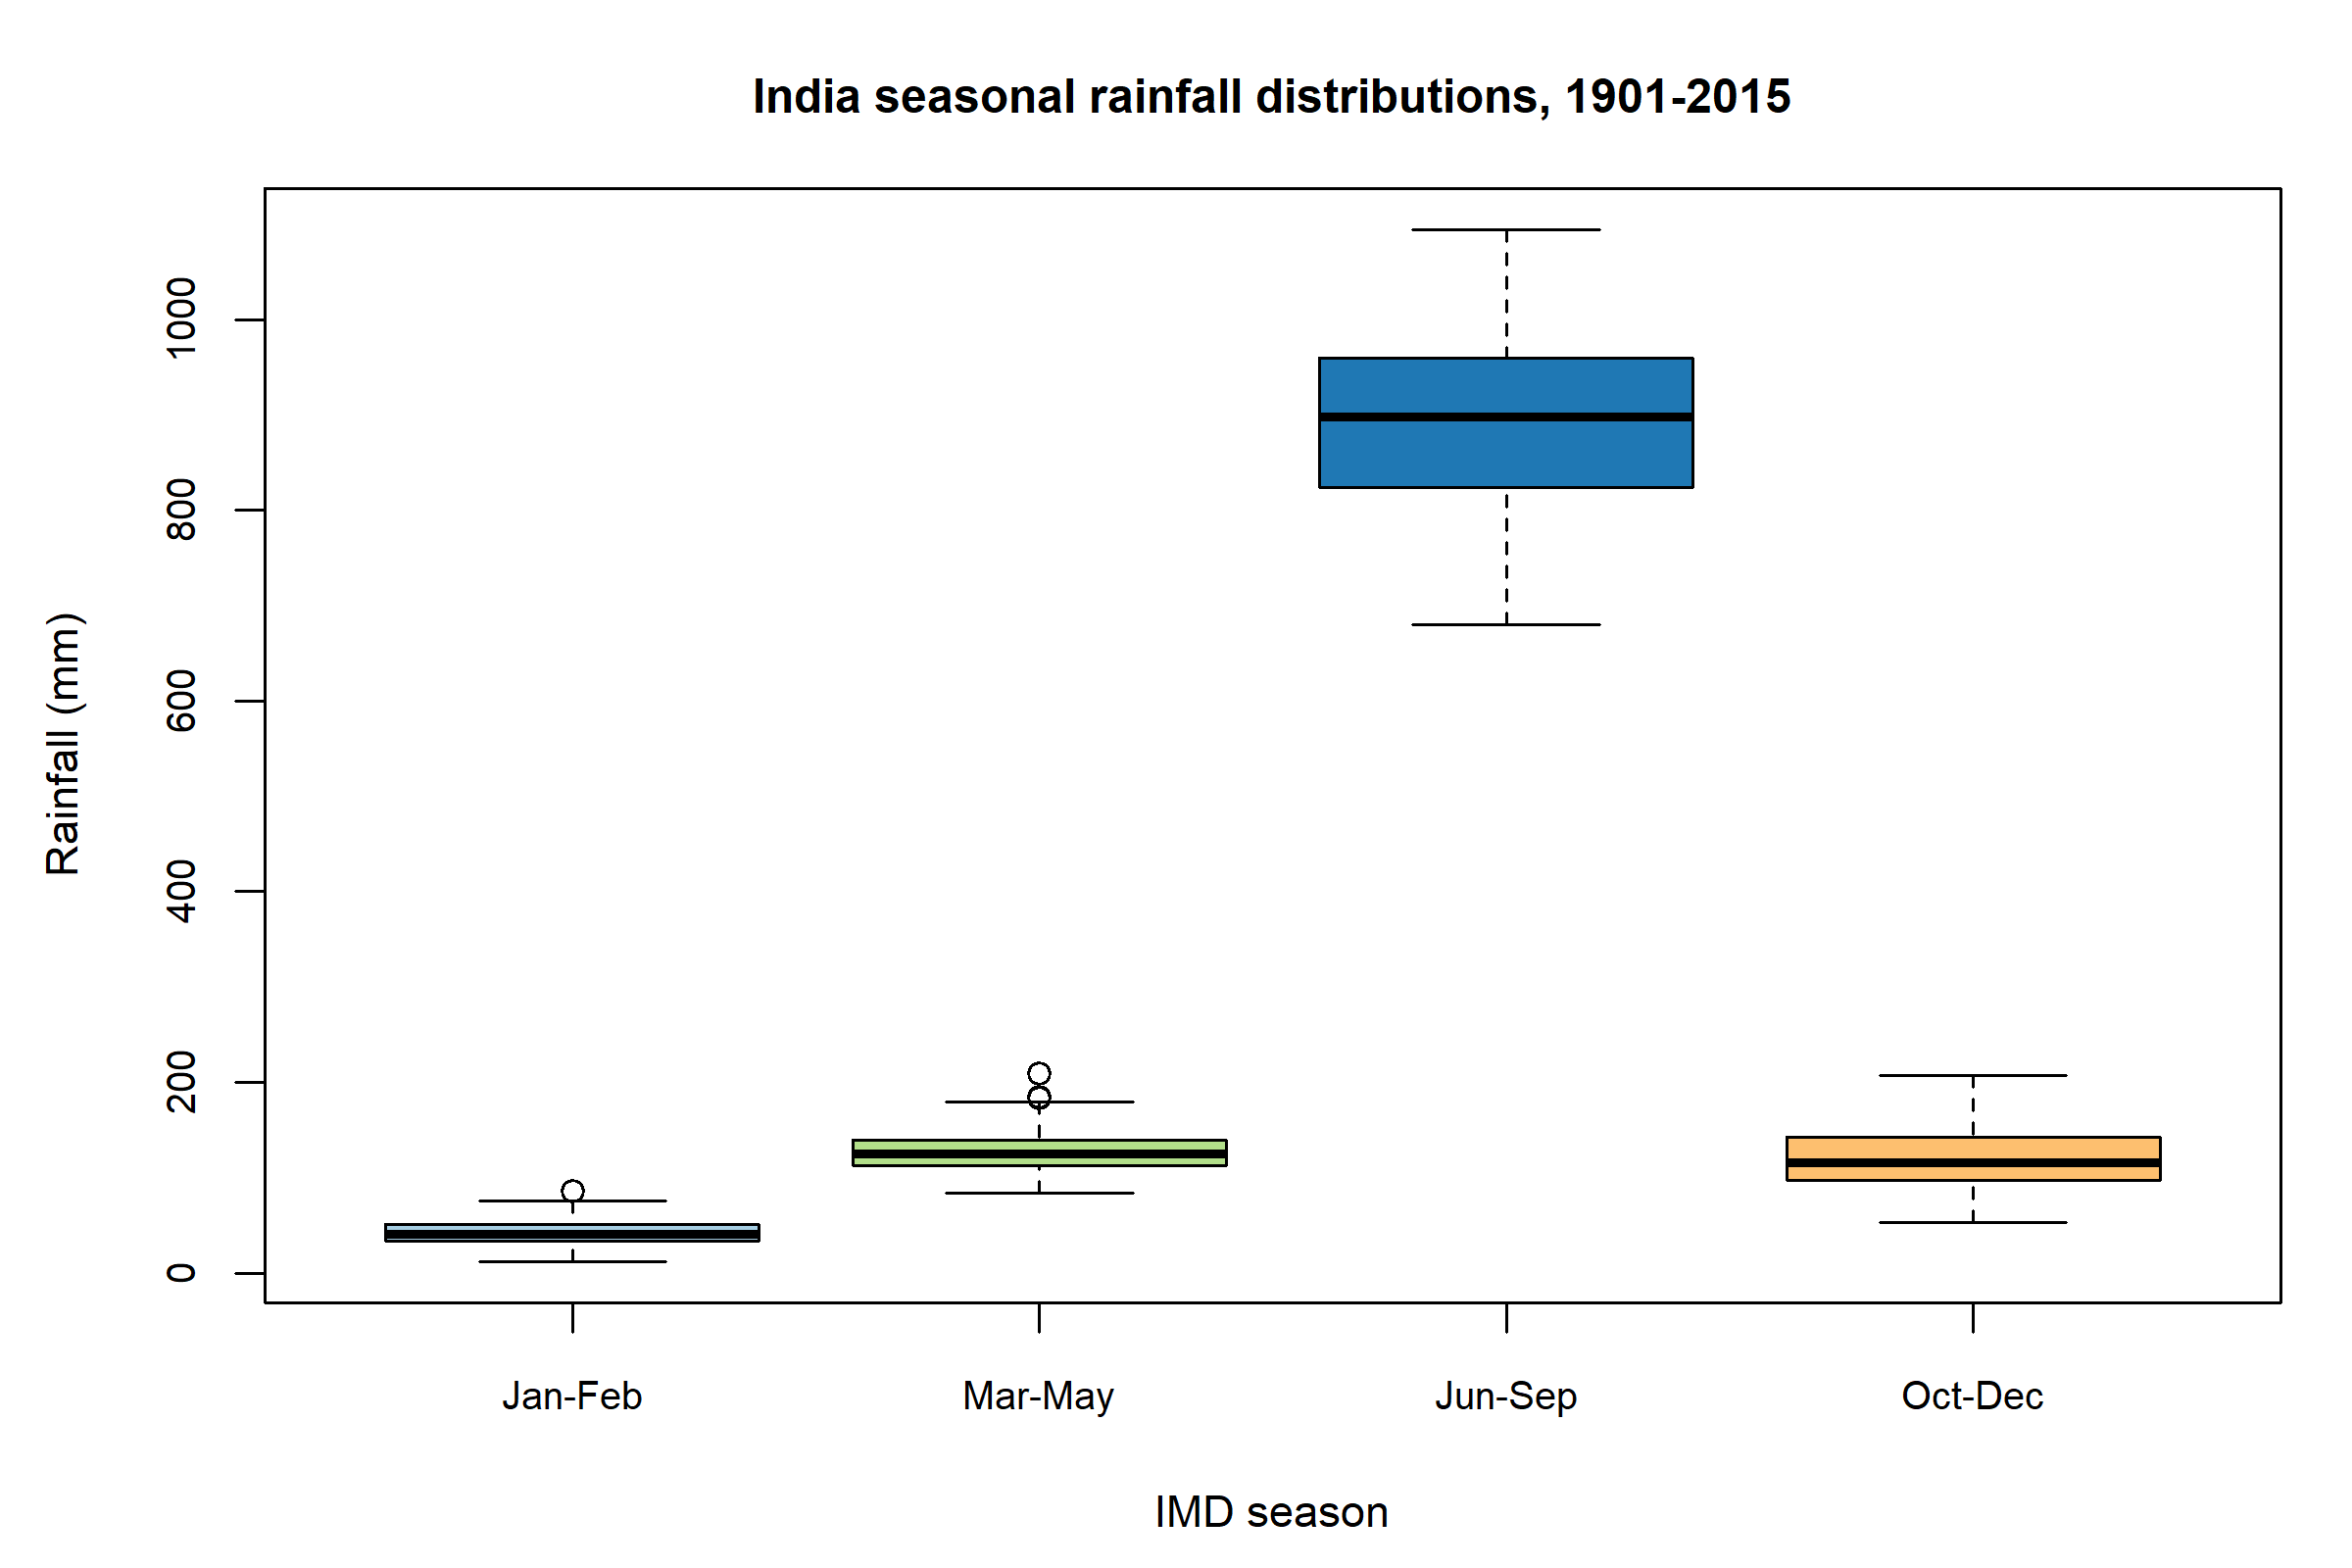
\includegraphics[width=0.92\linewidth]{../graphs/india_seasonal_boxplot} 

}

\caption{Figure 3. All-India seasonal rainfall distributions (mm), 1901–2015.}\label{fig:fig-season-box}
\end{figure}

Figures 2 and 3 make the same point visually: monsoon boxes sit far
above the other seasons, with no overlap of typical years.

Among subdivisions (complete years, 1901--2015), mean annual rainfall
runs from West Rajasthan (292.67 mm, CV 37.19\%) to very wet
western-coast and north-eastern subdivisions (Coastal Karnataka and
Arunachal Pradesh exceed 3400 mm). Kerala averages 2925.49 mm (CV
14.43\%). Drier regions tend to have \textbf{larger CVs}: relative
variability, not only the mean, differs by climate. Full regional tables
are in \texttt{results/tables/regional\_annual\_summaries.csv}.

\section{Probability and distribution
analysis}\label{probability-and-distribution-analysis}

\subsection{Empirical probabilities}\label{empirical-probabilities}

These quantities are \textbf{historical relative frequencies} in
1901--2015. They equal long-run probabilities only if one accepts extra
assumptions (a stationary process, a well-defined random year). They are
not forecasts.

The long-period average (LPA) analogue used here is the \textbf{sample
mean of this series}, not the official IMD 50-year LPA, which is not
stored in the CSV files. Deficient monsoon: June--September \(< 90\%\)
of that mean (801.23 mm). Excess: \(> 110\%\) (979.29 mm).

\begin{longtable}[]{@{}
  >{\raggedright\arraybackslash}p{(\linewidth - 8\tabcolsep) * \real{0.4329}}
  >{\raggedright\arraybackslash}p{(\linewidth - 8\tabcolsep) * \real{0.3171}}
  >{\raggedleft\arraybackslash}p{(\linewidth - 8\tabcolsep) * \real{0.0610}}
  >{\raggedleft\arraybackslash}p{(\linewidth - 8\tabcolsep) * \real{0.0732}}
  >{\raggedleft\arraybackslash}p{(\linewidth - 8\tabcolsep) * \real{0.1159}}@{}}
\caption{Table 4. Empirical probabilities, all-India, 1901--2015 (n =
115).}\tabularnewline
\toprule\noalign{}
\begin{minipage}[b]{\linewidth}\raggedright
Event
\end{minipage} & \begin{minipage}[b]{\linewidth}\raggedright
Definition
\end{minipage} & \begin{minipage}[b]{\linewidth}\raggedleft
Numerator
\end{minipage} & \begin{minipage}[b]{\linewidth}\raggedleft
Denominator
\end{minipage} & \begin{minipage}[b]{\linewidth}\raggedleft
Relative frequency
\end{minipage} \\
\midrule\noalign{}
\endfirsthead
\toprule\noalign{}
\begin{minipage}[b]{\linewidth}\raggedright
Event
\end{minipage} & \begin{minipage}[b]{\linewidth}\raggedright
Definition
\end{minipage} & \begin{minipage}[b]{\linewidth}\raggedleft
Numerator
\end{minipage} & \begin{minipage}[b]{\linewidth}\raggedleft
Denominator
\end{minipage} & \begin{minipage}[b]{\linewidth}\raggedleft
Relative frequency
\end{minipage} \\
\midrule\noalign{}
\endhead
\bottomrule\noalign{}
\endlastfoot
Annual rainfall greater than the 1901-2015 sample mean (LPA analogue) &
ANNUAL \textgreater{} 1182.03 mm & 59 & 115 & 0.513 \\
Unusually dry year (below historical 10th percentile) & ANNUAL
\textless{} 1041.30 mm (10th percentile of 1901-2015) & 12 & 115 &
0.104 \\
Unusually wet year (above historical 90th percentile) & ANNUAL
\textgreater{} 1331.30 mm (90th percentile of 1901-2015) & 12 & 115 &
0.104 \\
Deficient southwest monsoon (IMD-style: JJAS \textless{} 90\% of series
mean) & Jun-Sep \textless{} 0.90 * 890.26 mm & 25 & 115 & 0.217 \\
Normal southwest monsoon (90-110\% of series mean) & 0.90\emph{LPA
\textless= Jun-Sep \textless= 1.10}LPA & 74 & 115 & 0.643 \\
Excess southwest monsoon (JJAS \textgreater{} 110\% of series mean) &
Jun-Sep \textgreater{} 1.10 * 890.26 mm & 16 & 115 & 0.139 \\
Conditional: deficient monsoon given dry winter (JF \textless{} 25th
percentile) & P(JJAS deficient \textbar{} Jan-Feb \textless{} 33.80 mm)
& 6 & 29 & 0.207 \\
Conditional: deficient monsoon given not-dry winter & P(JJAS deficient
\textbar{} Jan-Feb \textgreater= 25th percentile) & 19 & 86 & 0.221 \\
Southwest monsoon is the wettest IMD season of the year & Jun-Sep ==
max(Jan-Feb, Mar-May, Jun-Sep, Oct-Dec) & 115 & 115 & 1.000 \\
\end{longtable}

About 64.3\% of years are ``normal'' under this rule, 21.7\% deficient
and 13.9\% excess. Unusually dry and wet \emph{annual} years, defined by
the sample 10th and 90th percentiles (1041.30 mm and 1331.30 mm), each
occur in 12 of 115 years by construction of a 10\% tail.

The conditional probability of a deficient monsoon given a dry winter
(January--February below its 25th percentile) is 0.207, versus 0.221
given a not-dry winter. The two frequencies are almost the same: this
record does \textbf{not} show a useful winter--monsoon dependence of
that form. That is association only, not a physical conclusion about
teleconnections.

In every one of the 115 years, June--September was the wettest of the
four IMD seasons (relative frequency 1).

\subsection{Probability models}\label{probability-models}

A normal law can assign probability to negative rainfall, so it is not
automatic for millimetres. A gamma law is supported on \((0,\infty)\)
and can be right-skewed. An exponential law is a gamma with shape 1 and
forces \(\mathrm{SD}=\mathrm{mean}\). For all-India annual rainfall, SD
(110.69 mm) is far smaller than the mean (1182.03 mm), so exponential is
scientifically implausible and is fitted only as a bad reference.

Parameters were estimated by maximum likelihood. Goodness-of-fit
\(p\)-values for KS tests with estimated parameters come from a
parametric bootstrap (\(B=400\)).

\begin{longtable}[]{@{}
  >{\raggedright\arraybackslash}p{(\linewidth - 18\tabcolsep) * \real{0.1250}}
  >{\raggedright\arraybackslash}p{(\linewidth - 18\tabcolsep) * \real{0.1161}}
  >{\raggedright\arraybackslash}p{(\linewidth - 18\tabcolsep) * \real{0.1071}}
  >{\raggedleft\arraybackslash}p{(\linewidth - 18\tabcolsep) * \real{0.0893}}
  >{\raggedright\arraybackslash}p{(\linewidth - 18\tabcolsep) * \real{0.1071}}
  >{\raggedleft\arraybackslash}p{(\linewidth - 18\tabcolsep) * \real{0.0982}}
  >{\raggedleft\arraybackslash}p{(\linewidth - 18\tabcolsep) * \real{0.0625}}
  >{\raggedleft\arraybackslash}p{(\linewidth - 18\tabcolsep) * \real{0.0714}}
  >{\raggedleft\arraybackslash}p{(\linewidth - 18\tabcolsep) * \real{0.1339}}
  >{\raggedleft\arraybackslash}p{(\linewidth - 18\tabcolsep) * \real{0.0893}}@{}}
\caption{Table 5. Fitted distributions. KS p-values are parametric
bootstrap, not ordinary ks.test p-values.}\tabularnewline
\toprule\noalign{}
\begin{minipage}[b]{\linewidth}\raggedright
series
\end{minipage} & \begin{minipage}[b]{\linewidth}\raggedright
distribution
\end{minipage} & \begin{minipage}[b]{\linewidth}\raggedright
param1\_name
\end{minipage} & \begin{minipage}[b]{\linewidth}\raggedleft
param1
\end{minipage} & \begin{minipage}[b]{\linewidth}\raggedright
param2\_name
\end{minipage} & \begin{minipage}[b]{\linewidth}\raggedleft
param2
\end{minipage} & \begin{minipage}[b]{\linewidth}\raggedleft
aic
\end{minipage} & \begin{minipage}[b]{\linewidth}\raggedleft
ks\_stat
\end{minipage} & \begin{minipage}[b]{\linewidth}\raggedleft
ks\_p\_bootstrap
\end{minipage} & \begin{minipage}[b]{\linewidth}\raggedleft
shapiro\_p
\end{minipage} \\
\midrule\noalign{}
\endfirsthead
\toprule\noalign{}
\begin{minipage}[b]{\linewidth}\raggedright
series
\end{minipage} & \begin{minipage}[b]{\linewidth}\raggedright
distribution
\end{minipage} & \begin{minipage}[b]{\linewidth}\raggedright
param1\_name
\end{minipage} & \begin{minipage}[b]{\linewidth}\raggedleft
param1
\end{minipage} & \begin{minipage}[b]{\linewidth}\raggedright
param2\_name
\end{minipage} & \begin{minipage}[b]{\linewidth}\raggedleft
param2
\end{minipage} & \begin{minipage}[b]{\linewidth}\raggedleft
aic
\end{minipage} & \begin{minipage}[b]{\linewidth}\raggedleft
ks\_stat
\end{minipage} & \begin{minipage}[b]{\linewidth}\raggedleft
ks\_p\_bootstrap
\end{minipage} & \begin{minipage}[b]{\linewidth}\raggedleft
shapiro\_p
\end{minipage} \\
\midrule\noalign{}
\endhead
\bottomrule\noalign{}
\endlastfoot
India annual & gamma & shape & 114.0443 & rate & 0.09648 & 1412.3 &
0.0612 & 0.3725 & 0.8014 \\
India annual & normal & mean & 1182.0348 & sd\_mle & 110.20392 & 1411.9
& 0.0517 & 0.6100 & 0.8014 \\
India annual & exponential & rate & 0.0008 & mean & 1182.03478 & 1859.2
& 0.5411 & 0.0000 & 0.8014 \\
India Jun-Sep & gamma & shape & 97.5089 & rate & 0.10953 & 1364.9 &
0.1155 & 0.0000 & 0.0581 \\
\end{longtable}

For \textbf{all-India annual} rainfall, Shapiro--Wilk \(W=\) 0.9926,
\(p=\) 0.8014: the normal model is not rejected. Bootstrap KS \(p=\)
0.6100 (normal) and \(p=\) 0.3725 (gamma). AIC slightly favours the
normal (1411.9) over the gamma (1412.3). Exponential AIC is 1859.2 and
bootstrap KS \(p=\) \textless{} 0.0001: it is rejected.

The gamma MLE for annual totals is shape \(\hat\alpha=\) 114.04 and rate
\(\hat\beta=\) 0.0965 mm\(^{-1}\). A large shape is consistent with a
nearly symmetric, peaked distribution, which matches the small sample
skewness.

June--September is slightly left-skewed (skewness -0.294). A
right-skewed gamma is therefore a poorer match: bootstrap KS \(p=\)
\textless{} 0.0001 and Shapiro--Wilk \(p=\) 0.0581. That is a limitation
of forcing a gamma onto monsoon totals, not a reason to switch to
exponential.

\begin{figure}

{\centering 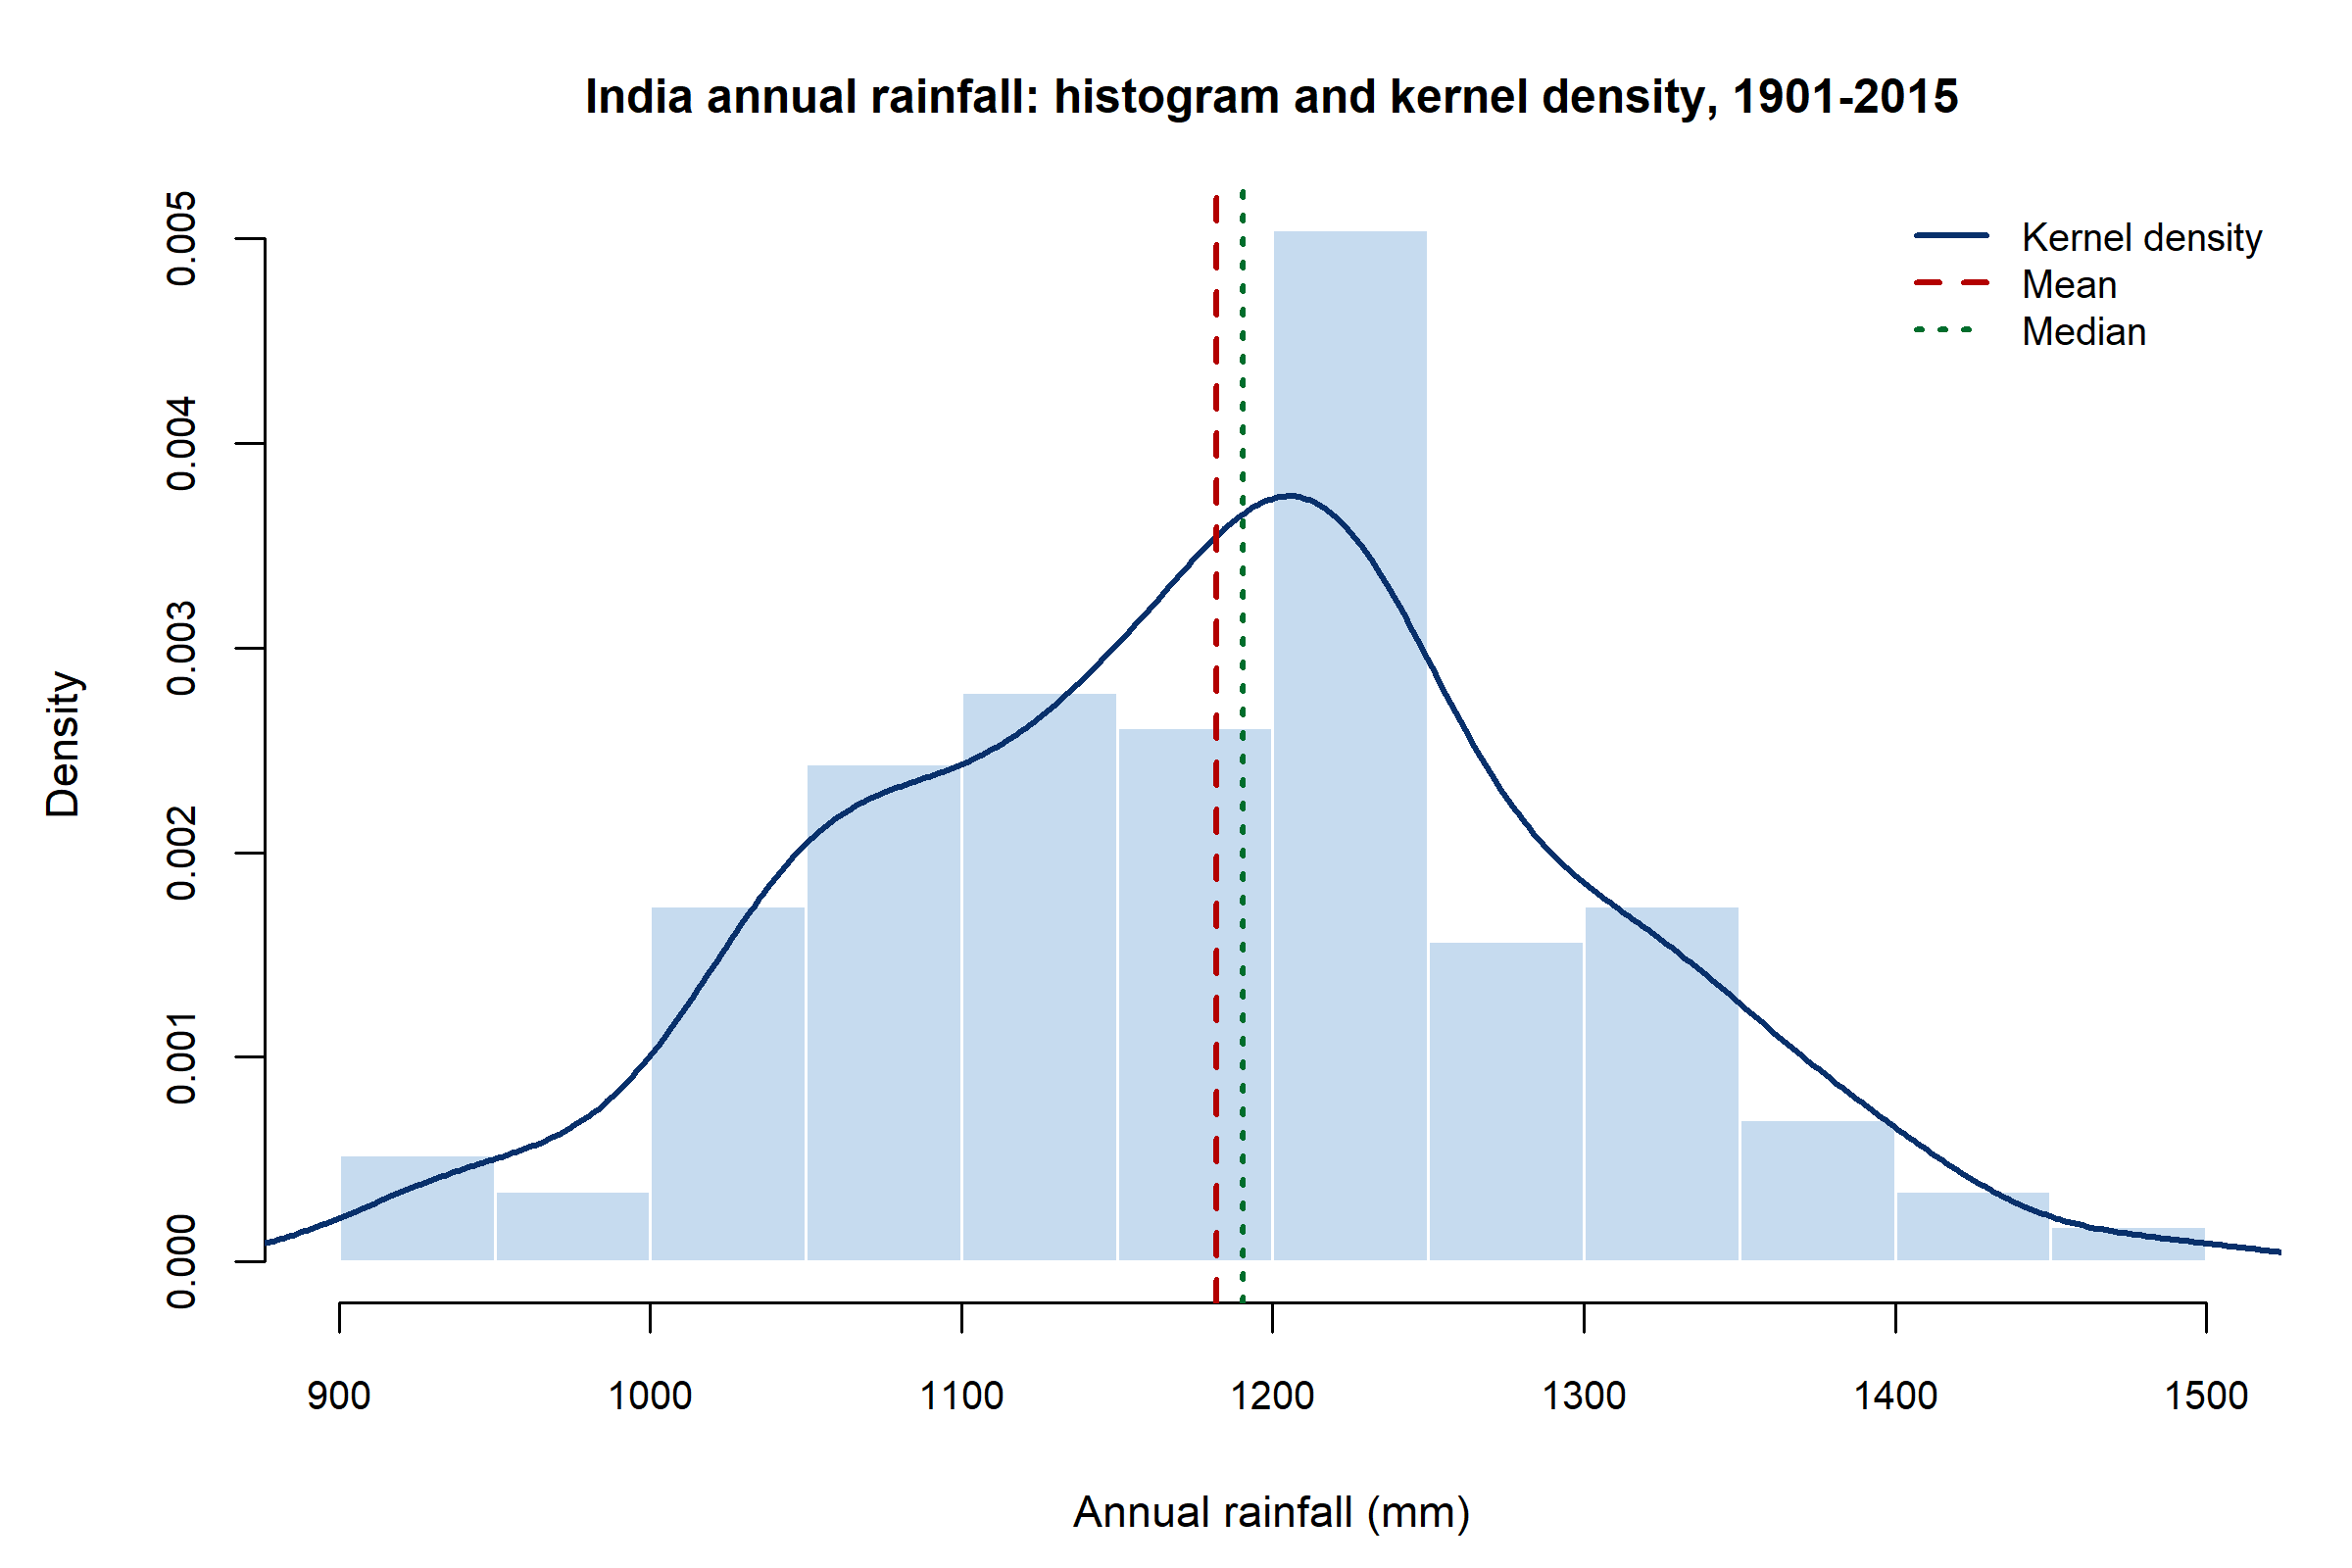
\includegraphics[width=0.92\linewidth]{../graphs/india_annual_histogram_density} 

}

\caption{Figure 4. Histogram and kernel density of all-India annual rainfall (mm), 1901–2015.}\label{fig:fig-hist}
\end{figure}

\begin{figure}

{\centering 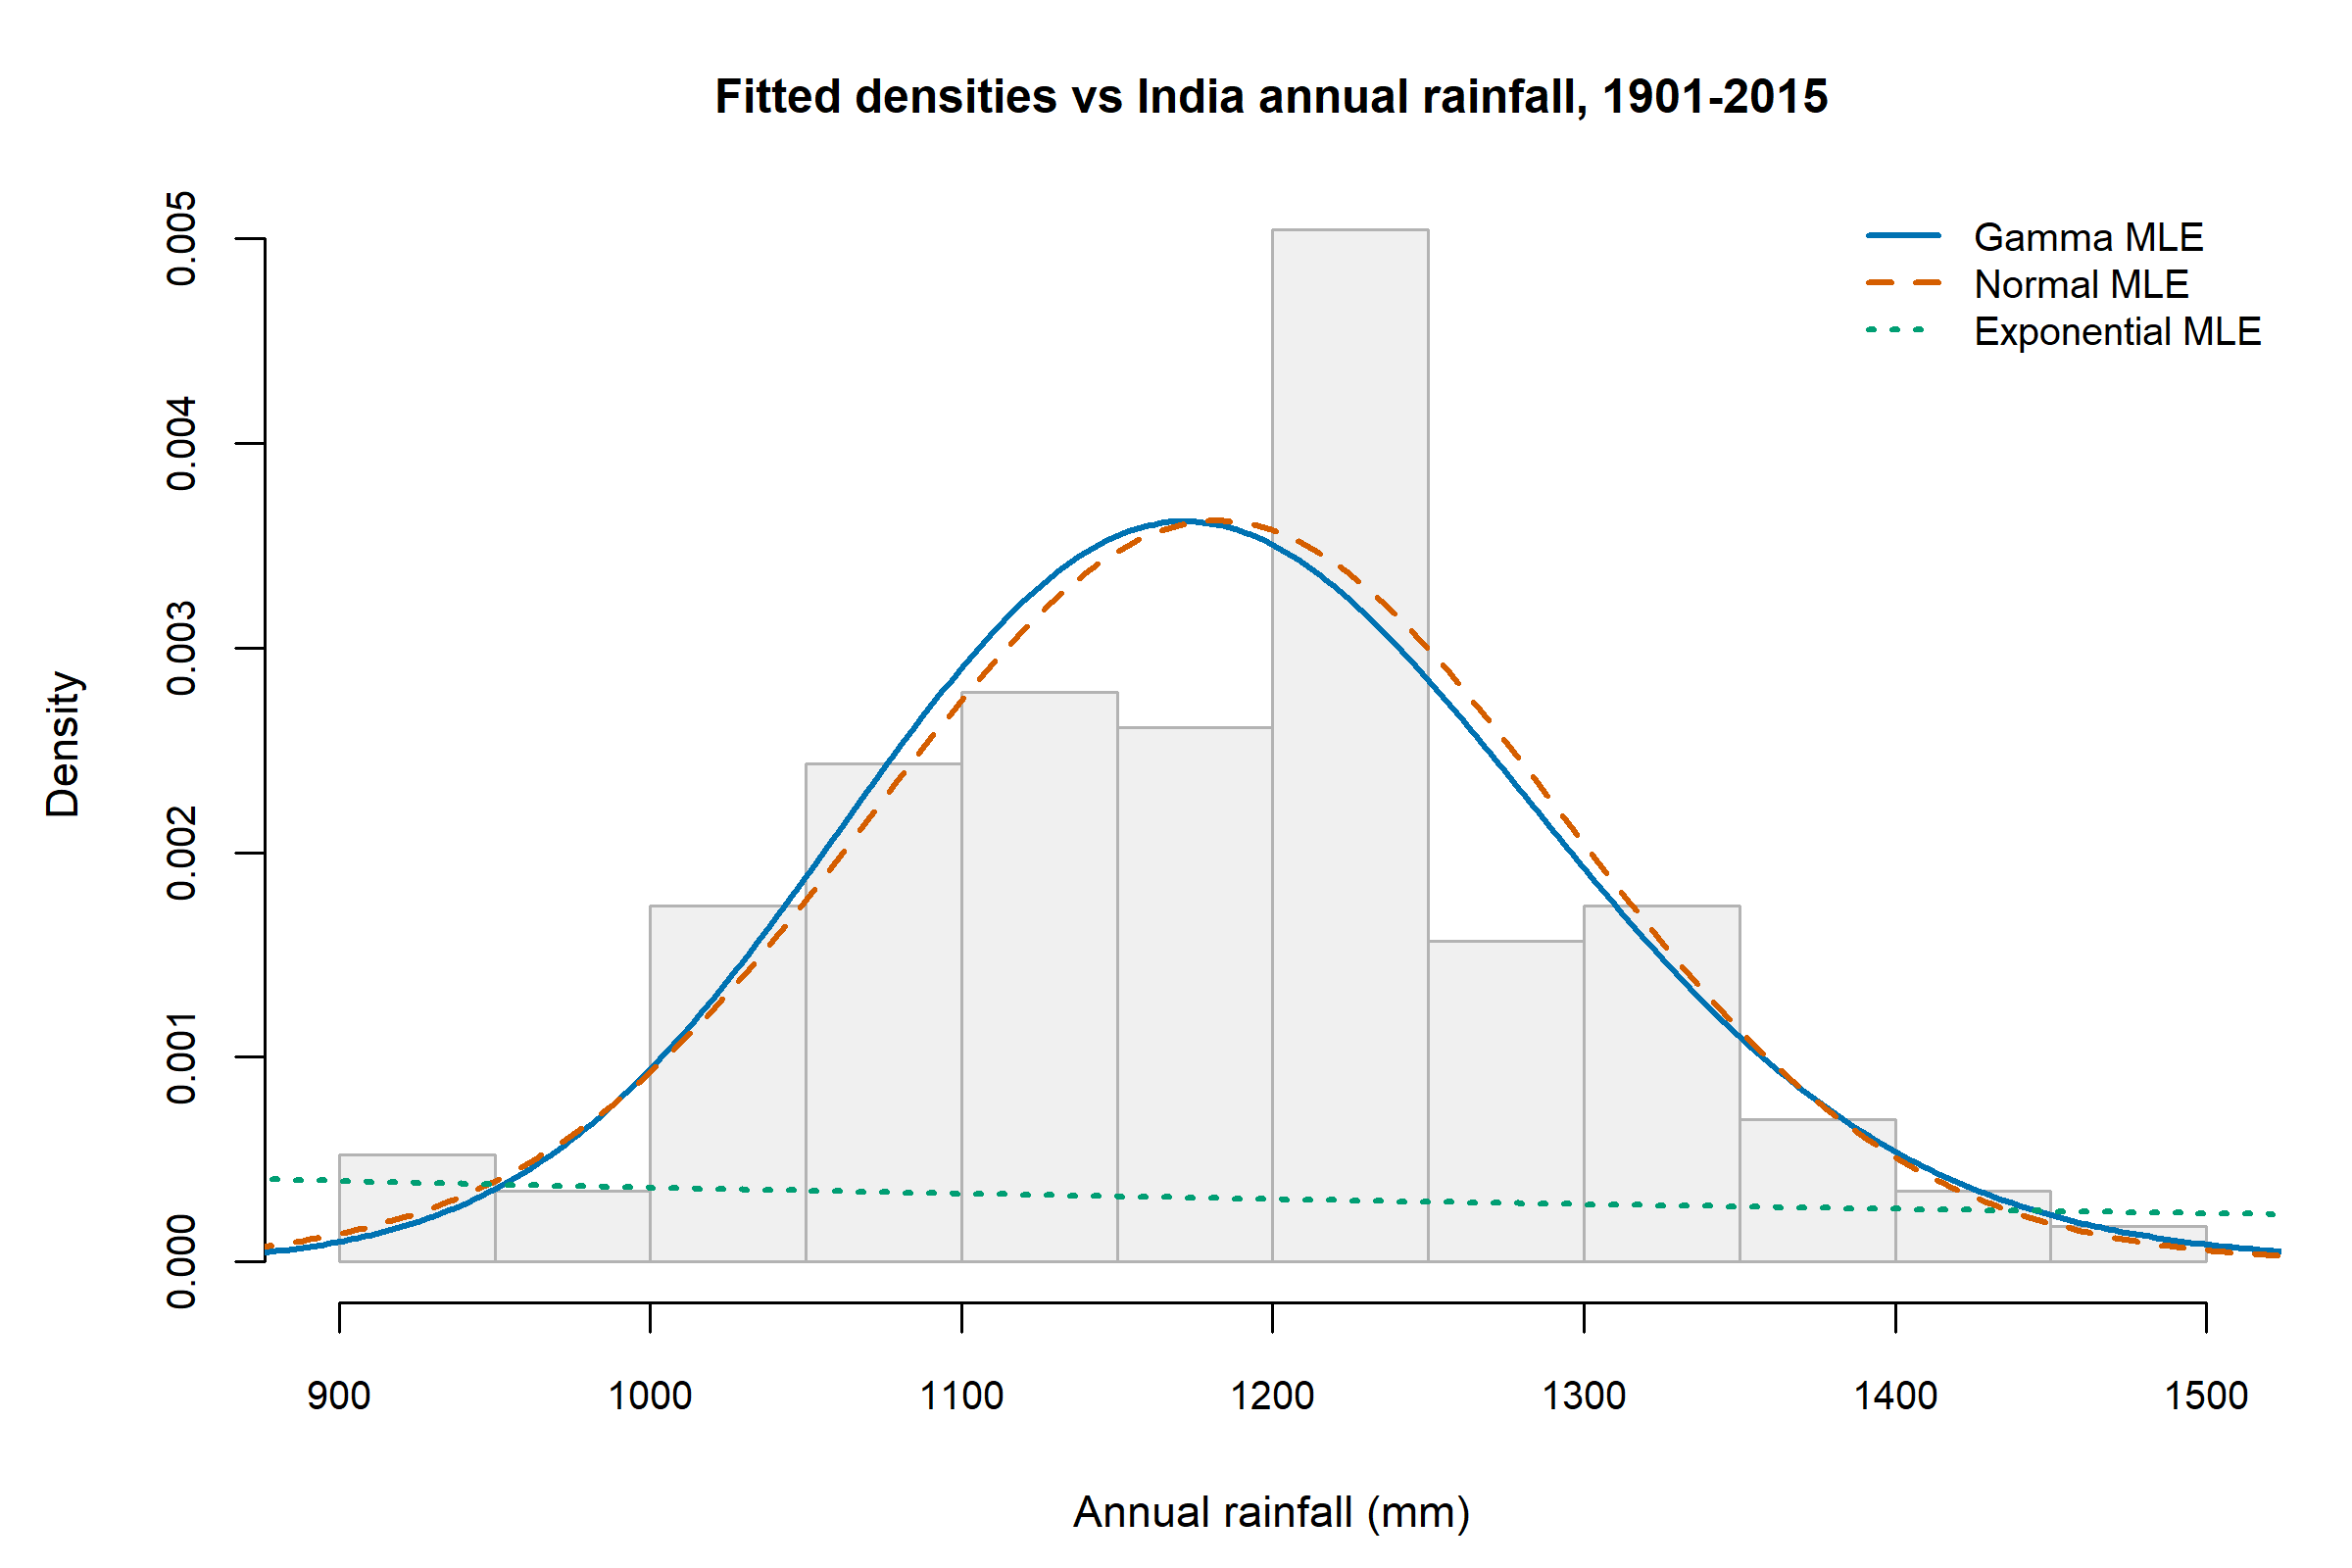
\includegraphics[width=0.92\linewidth]{../graphs/india_annual_distribution_overlay} 

}

\caption{Figure 5. Gamma, normal and exponential densities fitted to all-India annual rainfall.}\label{fig:fig-overlay}
\end{figure}

\begin{figure}

{\centering 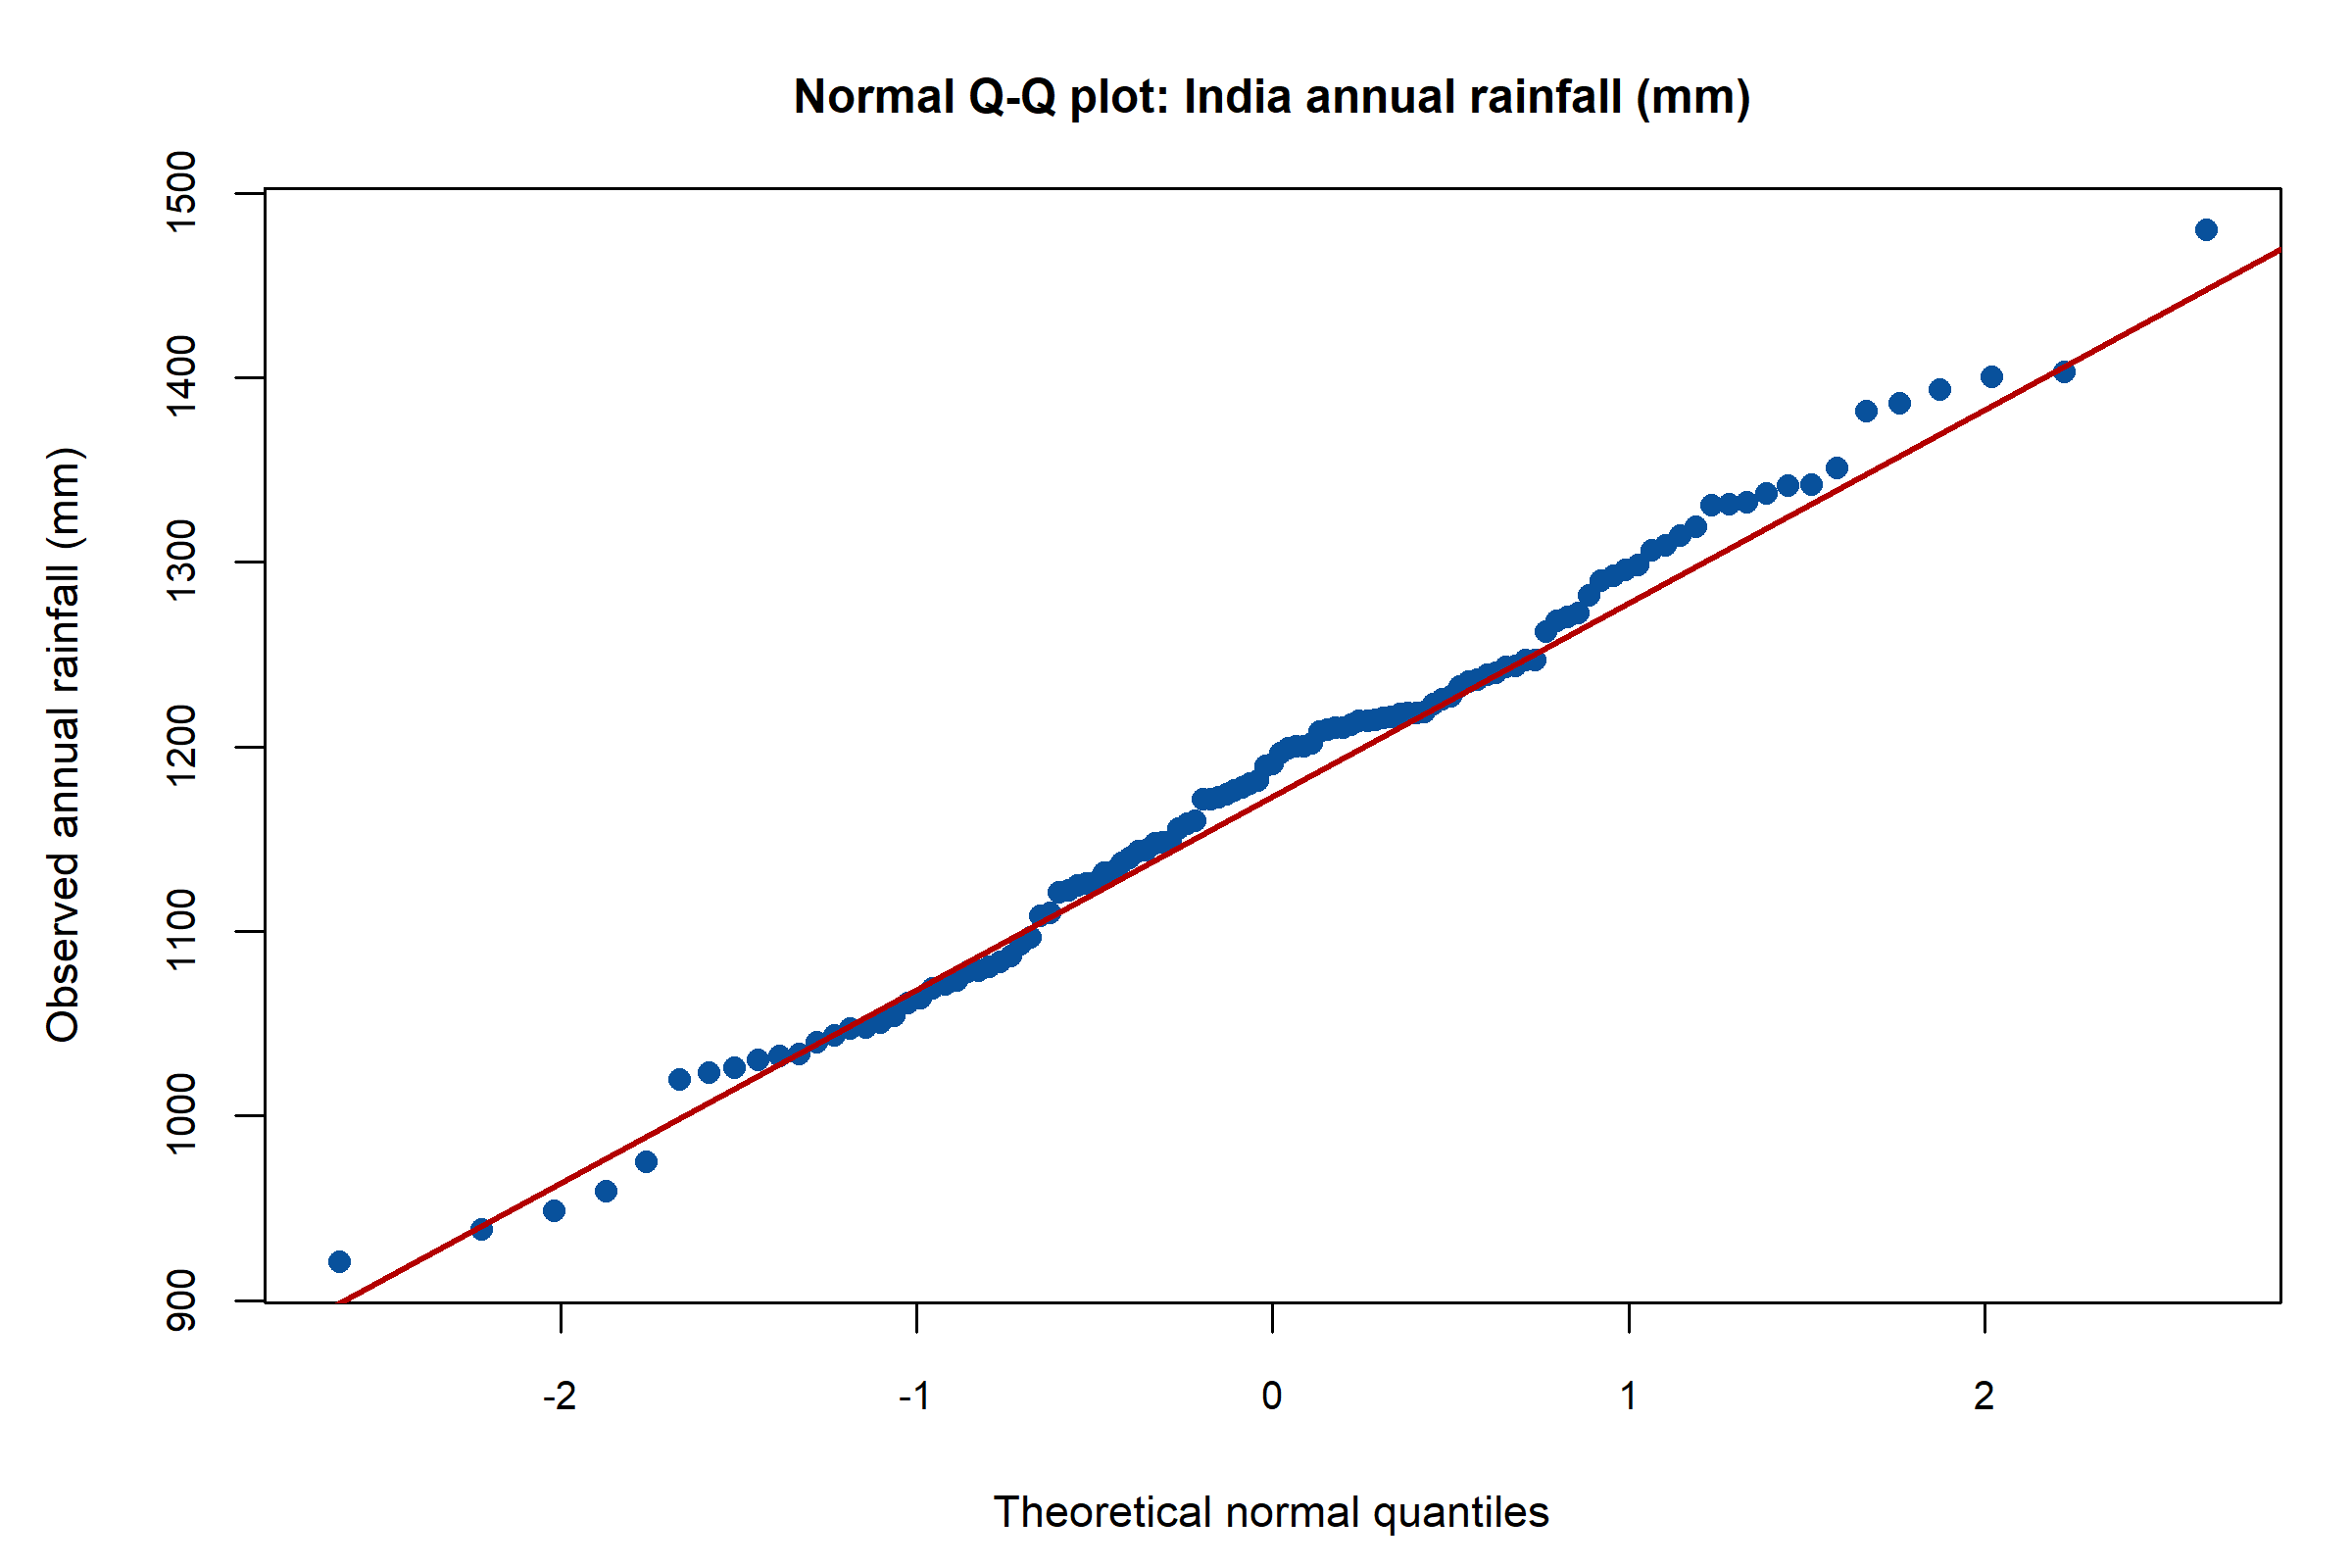
\includegraphics[width=0.92\linewidth]{../graphs/india_annual_qq_normal} 

}

\caption{Figure 6. Normal Q–Q plot of all-India annual rainfall (mm).}\label{fig:fig-qqn}
\end{figure}

\begin{figure}

{\centering 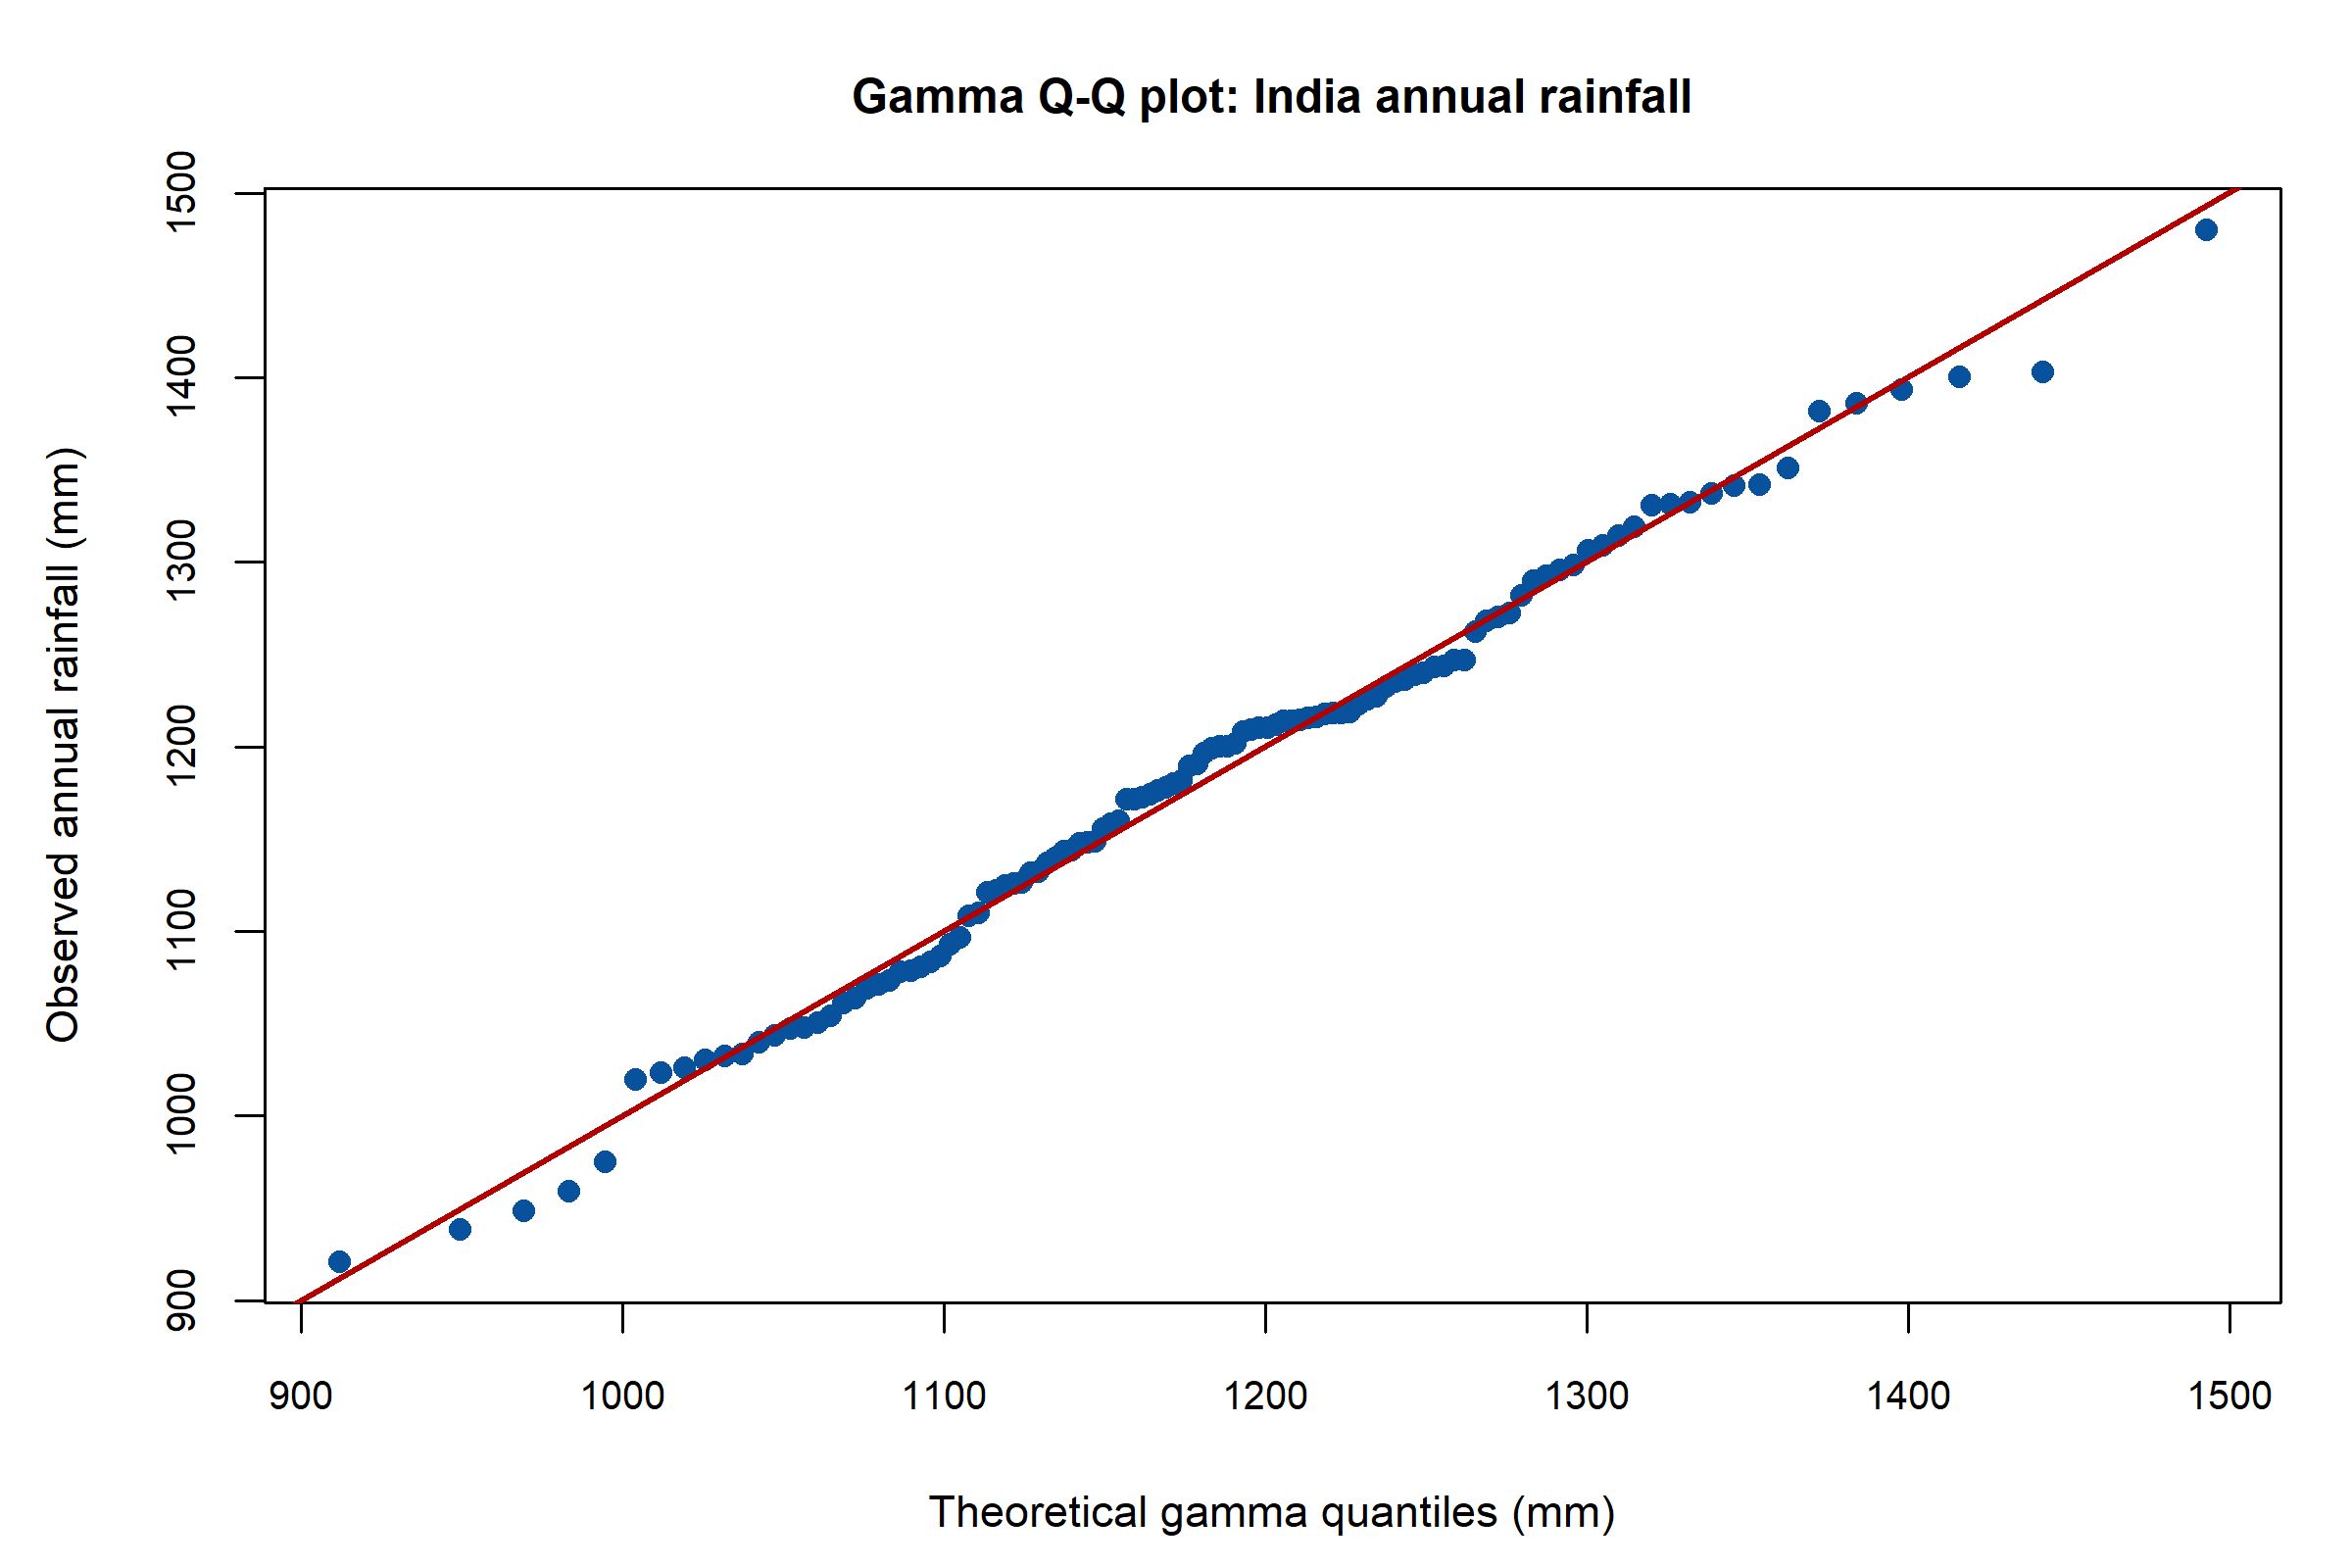
\includegraphics[width=0.92\linewidth]{../graphs/india_annual_qq_gamma} 

}

\caption{Figure 7. Gamma Q–Q plot of all-India annual rainfall (mm).}\label{fig:fig-qqg}
\end{figure}

\begin{figure}

{\centering 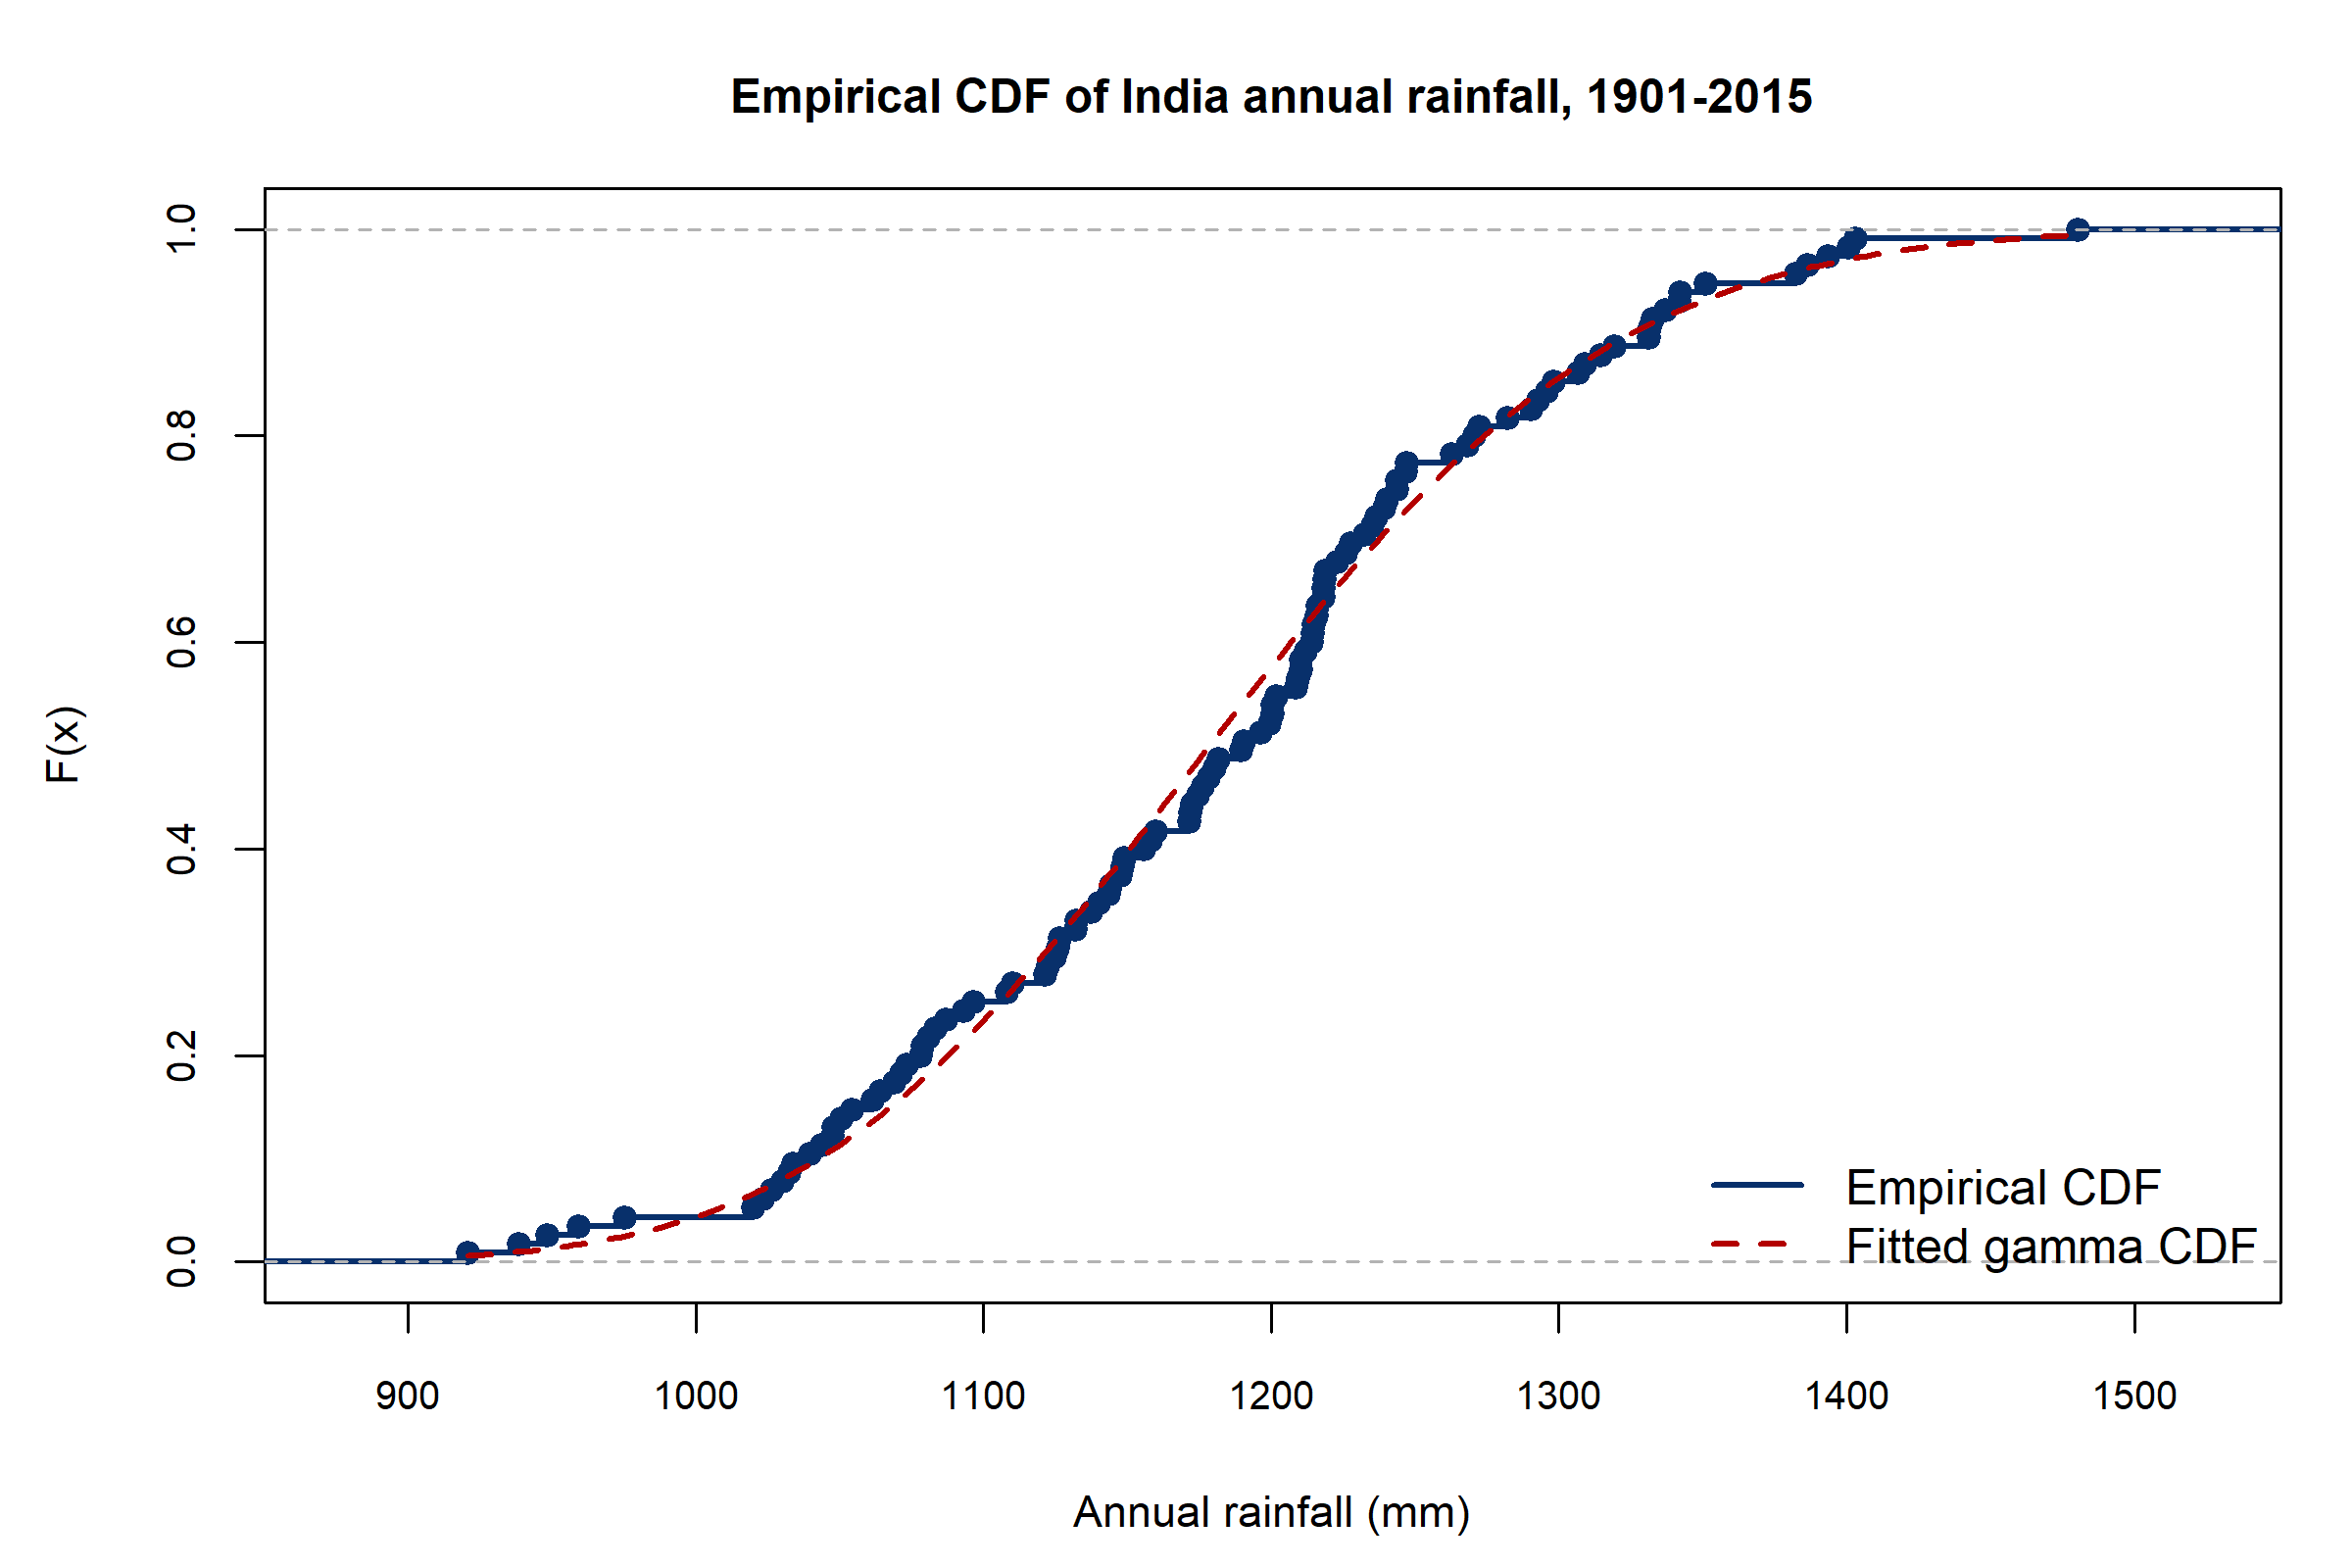
\includegraphics[width=0.92\linewidth]{../graphs/india_annual_ecdf} 

}

\caption{Figure 8. Empirical CDF of all-India annual rainfall with the fitted gamma CDF.}\label{fig:fig-ecdf}
\end{figure}

Figures 4--8 agree with Table 5: the histogram is unimodal and fairly
symmetric; exponential is far too spread out; normal and gamma Q--Q
plots are both reasonable.

\textbf{Zeros.} The national monthly series has no zeros. Subdivision
dry-season months do. A single gamma or exponential cannot place a point
mass at zero. For West Rajasthan December (complete years, \(n=\) 117),
43 months are zero, so the empirical \(P(X=0)=\) 0.368. Positive amounts
were given a separate gamma (shape 0.654, rate 0.219). This is a hurdle
description, not a claim that December rain is a waiting time.

\section{Sampling and estimation}\label{sampling-and-estimation}

The 115 years are \textbf{one realised path} of a climate process.
Treating them as iid draws from a super-population is an approximation
used to illustrate textbook sampling theory.

The estimated standard error of the all-India annual mean is
\(s/\sqrt{n}=\) 10.32 mm.

A teaching simulation (seed 19012015) drew 4000 bootstrap samples
\textbf{with replacement from the 115 observed annual totals}, for
sample sizes 5, 15 and 40. These draws are \textbf{not extra
meteorological years} and must not be averaged into the data.

\begin{longtable}[]{@{}
  >{\raggedleft\arraybackslash}p{(\linewidth - 12\tabcolsep) * \real{0.1053}}
  >{\raggedleft\arraybackslash}p{(\linewidth - 12\tabcolsep) * \real{0.1316}}
  >{\raggedleft\arraybackslash}p{(\linewidth - 12\tabcolsep) * \real{0.1842}}
  >{\raggedleft\arraybackslash}p{(\linewidth - 12\tabcolsep) * \real{0.1667}}
  >{\raggedleft\arraybackslash}p{(\linewidth - 12\tabcolsep) * \real{0.1316}}
  >{\raggedleft\arraybackslash}p{(\linewidth - 12\tabcolsep) * \real{0.1579}}
  >{\raggedleft\arraybackslash}p{(\linewidth - 12\tabcolsep) * \real{0.1228}}@{}}
\caption{Table 6. CLT resampling demonstration from the empirical
all-India annual distribution (4000 replications).}\tabularnewline
\toprule\noalign{}
\begin{minipage}[b]{\linewidth}\raggedleft
sample\_size
\end{minipage} & \begin{minipage}[b]{\linewidth}\raggedleft
n\_replications
\end{minipage} & \begin{minipage}[b]{\linewidth}\raggedleft
mean\_of\_sample\_means
\end{minipage} & \begin{minipage}[b]{\linewidth}\raggedleft
sd\_of\_sample\_means
\end{minipage} & \begin{minipage}[b]{\linewidth}\raggedleft
theoretical\_se
\end{minipage} & \begin{minipage}[b]{\linewidth}\raggedleft
skewness\_of\_means
\end{minipage} & \begin{minipage}[b]{\linewidth}\raggedleft
shapiro\_p\_500
\end{minipage} \\
\midrule\noalign{}
\endfirsthead
\toprule\noalign{}
\begin{minipage}[b]{\linewidth}\raggedleft
sample\_size
\end{minipage} & \begin{minipage}[b]{\linewidth}\raggedleft
n\_replications
\end{minipage} & \begin{minipage}[b]{\linewidth}\raggedleft
mean\_of\_sample\_means
\end{minipage} & \begin{minipage}[b]{\linewidth}\raggedleft
sd\_of\_sample\_means
\end{minipage} & \begin{minipage}[b]{\linewidth}\raggedleft
theoretical\_se
\end{minipage} & \begin{minipage}[b]{\linewidth}\raggedleft
skewness\_of\_means
\end{minipage} & \begin{minipage}[b]{\linewidth}\raggedleft
shapiro\_p\_500
\end{minipage} \\
\midrule\noalign{}
\endhead
\bottomrule\noalign{}
\endlastfoot
5 & 4000 & 1182.007 & 49.270 & 49.500 & 0.001 & 0.425 \\
15 & 4000 & 1181.403 & 28.530 & 28.579 & 0.020 & 0.547 \\
40 & 4000 & 1182.223 & 17.351 & 17.501 & -0.013 & 0.598 \\
\end{longtable}

\begin{figure}

{\centering 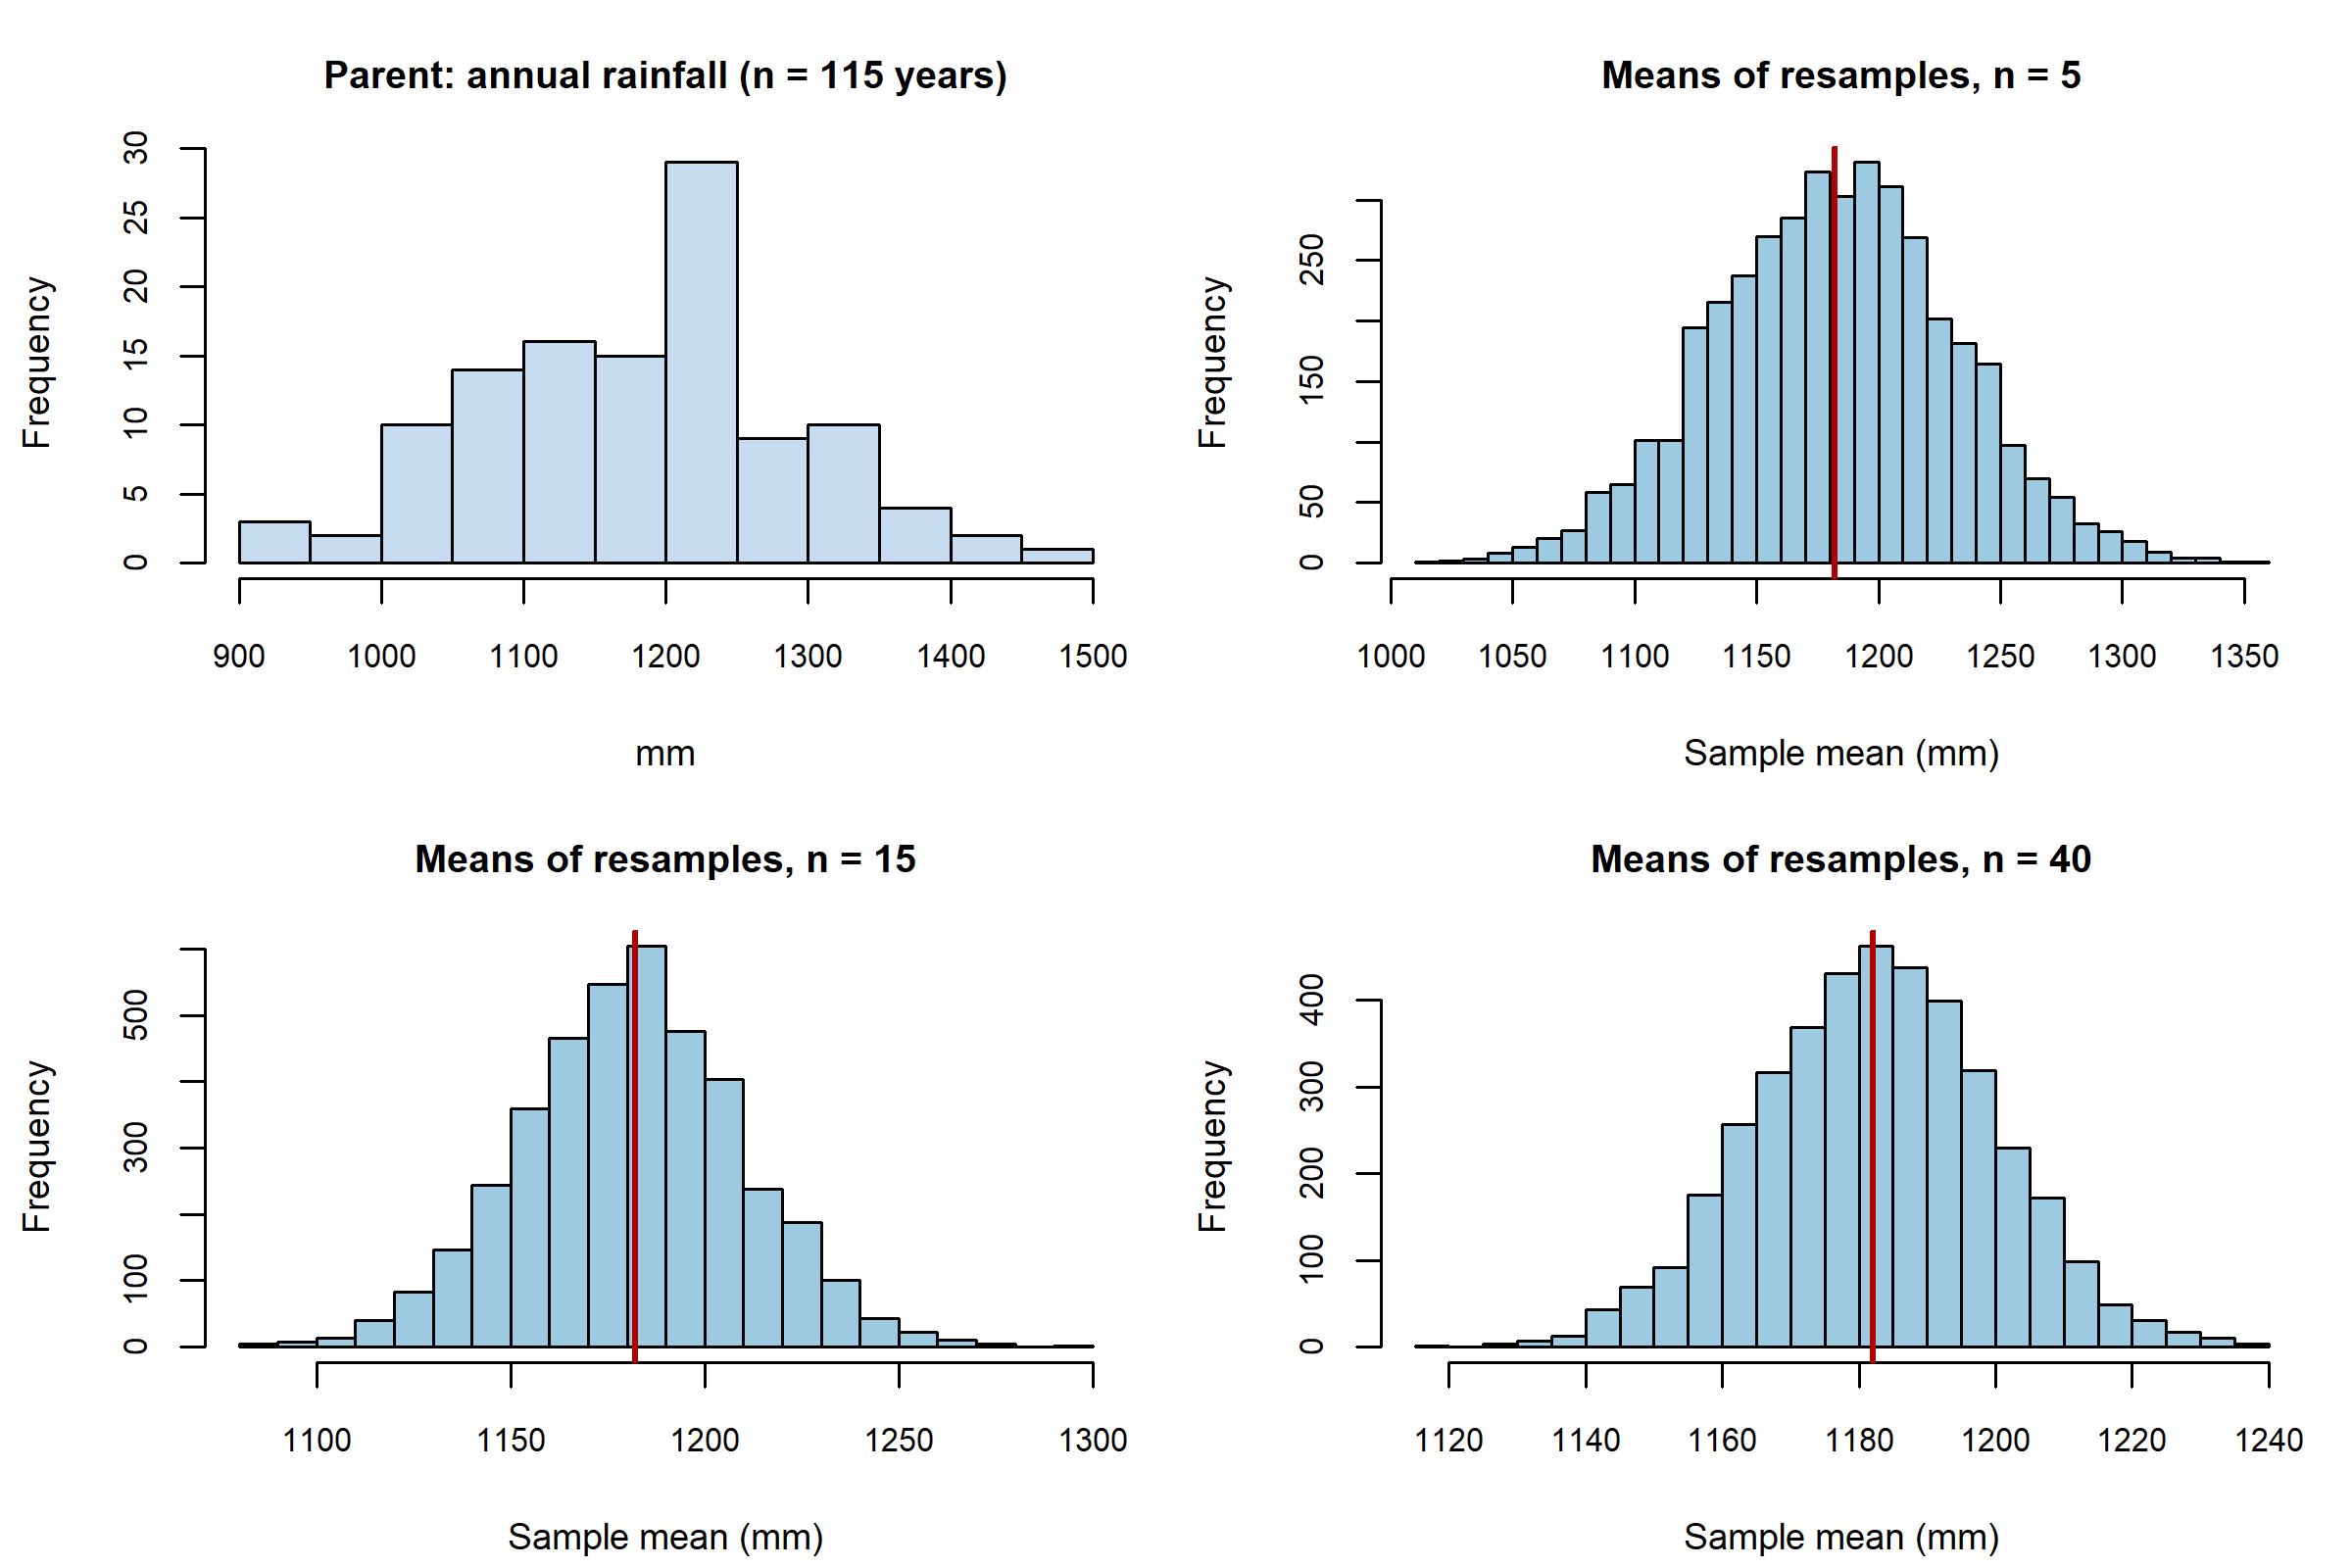
\includegraphics[width=0.92\linewidth]{../graphs/clt_sampling_distributions} 

}

\caption{Figure 9. Parent annual-rainfall histogram and sampling distributions of the mean for n = 5, 15 and 40. Simulated draws are teaching devices, not new observations.}\label{fig:fig-clt}
\end{figure}

As \(n\) grows, the histogram of sample means concentrates at about
1182.03 mm and the simulated SD of means tracks \(s/\sqrt{n}\) (for
\(n=40\), 17.35 mm versus theoretical 17.50 mm). Skewness of the means
is near zero. This is the Central Limit Theorem in a resampling
illustration, not a proof that annual climate is iid.

\section{Confidence intervals}\label{confidence-intervals}

\textbf{Parameter.} The mean of all-India area-weighted annual rainfall,
in millimetres, for the 1901--2015 record under the iid-normal (or CLT)
approximation.

\textbf{Method.} Student's \(t\) with \(n-1=114\) degrees of freedom.
Assumptions: independent years and either normality or a large-sample
mean. Shapiro--Wilk did not reject normality of annual totals, but lag-2
autocorrelation (Section 18) means the reported intervals are
\textbf{iid-benchmark} intervals and may be slightly too narrow.

\begin{longtable}[]{@{}
  >{\raggedright\arraybackslash}p{(\linewidth - 16\tabcolsep) * \real{0.1714}}
  >{\raggedright\arraybackslash}p{(\linewidth - 16\tabcolsep) * \real{0.2457}}
  >{\raggedleft\arraybackslash}p{(\linewidth - 16\tabcolsep) * \real{0.0971}}
  >{\raggedleft\arraybackslash}p{(\linewidth - 16\tabcolsep) * \real{0.0229}}
  >{\raggedleft\arraybackslash}p{(\linewidth - 16\tabcolsep) * \real{0.0514}}
  >{\raggedleft\arraybackslash}p{(\linewidth - 16\tabcolsep) * \real{0.0400}}
  >{\raggedleft\arraybackslash}p{(\linewidth - 16\tabcolsep) * \real{0.0457}}
  >{\raggedleft\arraybackslash}p{(\linewidth - 16\tabcolsep) * \real{0.0457}}
  >{\raggedright\arraybackslash}p{(\linewidth - 16\tabcolsep) * \real{0.2800}}@{}}
\caption{Table 7. Confidence intervals. Mean intervals are Student t;
proportion intervals are Wald.}\tabularnewline
\toprule\noalign{}
\begin{minipage}[b]{\linewidth}\raggedright
series
\end{minipage} & \begin{minipage}[b]{\linewidth}\raggedright
parameter
\end{minipage} & \begin{minipage}[b]{\linewidth}\raggedleft
confidence\_level
\end{minipage} & \begin{minipage}[b]{\linewidth}\raggedleft
n
\end{minipage} & \begin{minipage}[b]{\linewidth}\raggedleft
estimate
\end{minipage} & \begin{minipage}[b]{\linewidth}\raggedleft
se
\end{minipage} & \begin{minipage}[b]{\linewidth}\raggedleft
lower
\end{minipage} & \begin{minipage}[b]{\linewidth}\raggedleft
upper
\end{minipage} & \begin{minipage}[b]{\linewidth}\raggedright
method
\end{minipage} \\
\midrule\noalign{}
\endfirsthead
\toprule\noalign{}
\begin{minipage}[b]{\linewidth}\raggedright
series
\end{minipage} & \begin{minipage}[b]{\linewidth}\raggedright
parameter
\end{minipage} & \begin{minipage}[b]{\linewidth}\raggedleft
confidence\_level
\end{minipage} & \begin{minipage}[b]{\linewidth}\raggedleft
n
\end{minipage} & \begin{minipage}[b]{\linewidth}\raggedleft
estimate
\end{minipage} & \begin{minipage}[b]{\linewidth}\raggedleft
se
\end{minipage} & \begin{minipage}[b]{\linewidth}\raggedleft
lower
\end{minipage} & \begin{minipage}[b]{\linewidth}\raggedleft
upper
\end{minipage} & \begin{minipage}[b]{\linewidth}\raggedright
method
\end{minipage} \\
\midrule\noalign{}
\endhead
\bottomrule\noalign{}
\endlastfoot
India annual rainfall & mean (mm) & 0.90 & 115 & 1182.03 & 10.322 &
1164.92 & 1199.15 & Student t, iid assumption \\
India annual rainfall & mean (mm) & 0.95 & 115 & 1182.03 & 10.322 &
1161.59 & 1202.48 & Student t, iid assumption \\
India annual rainfall & mean (mm) & 0.99 & 115 & 1182.03 & 10.322 &
1155.00 & 1209.07 & Student t, iid assumption \\
India Jun-Sep rainfall & mean (mm) & 0.90 & 115 & 890.26 & 8.316 &
876.47 & 904.05 & Student t, iid assumption \\
India Jun-Sep rainfall & mean (mm) & 0.95 & 115 & 890.26 & 8.316 &
873.79 & 906.73 & Student t, iid assumption \\
India Jun-Sep rainfall & mean (mm) & 0.99 & 115 & 890.26 & 8.316 &
868.48 & 912.05 & Student t, iid assumption \\
India Jun-Sep deficient years & proportion deficient (\textless90\% of
series mean) & 0.90 & 115 & 0.22 & 0.038 & 0.15 & 0.28 & Wald (normal)
interval for a binomial proportion \\
India Jun-Sep deficient years & proportion deficient (\textless90\% of
series mean) & 0.95 & 115 & 0.22 & 0.038 & 0.14 & 0.29 & Wald (normal)
interval for a binomial proportion \\
India Jun-Sep deficient years & proportion deficient (\textless90\% of
series mean) & 0.99 & 115 & 0.22 & 0.038 & 0.12 & 0.32 & Wald (normal)
interval for a binomial proportion \\
\end{longtable}

\begin{figure}

{\centering 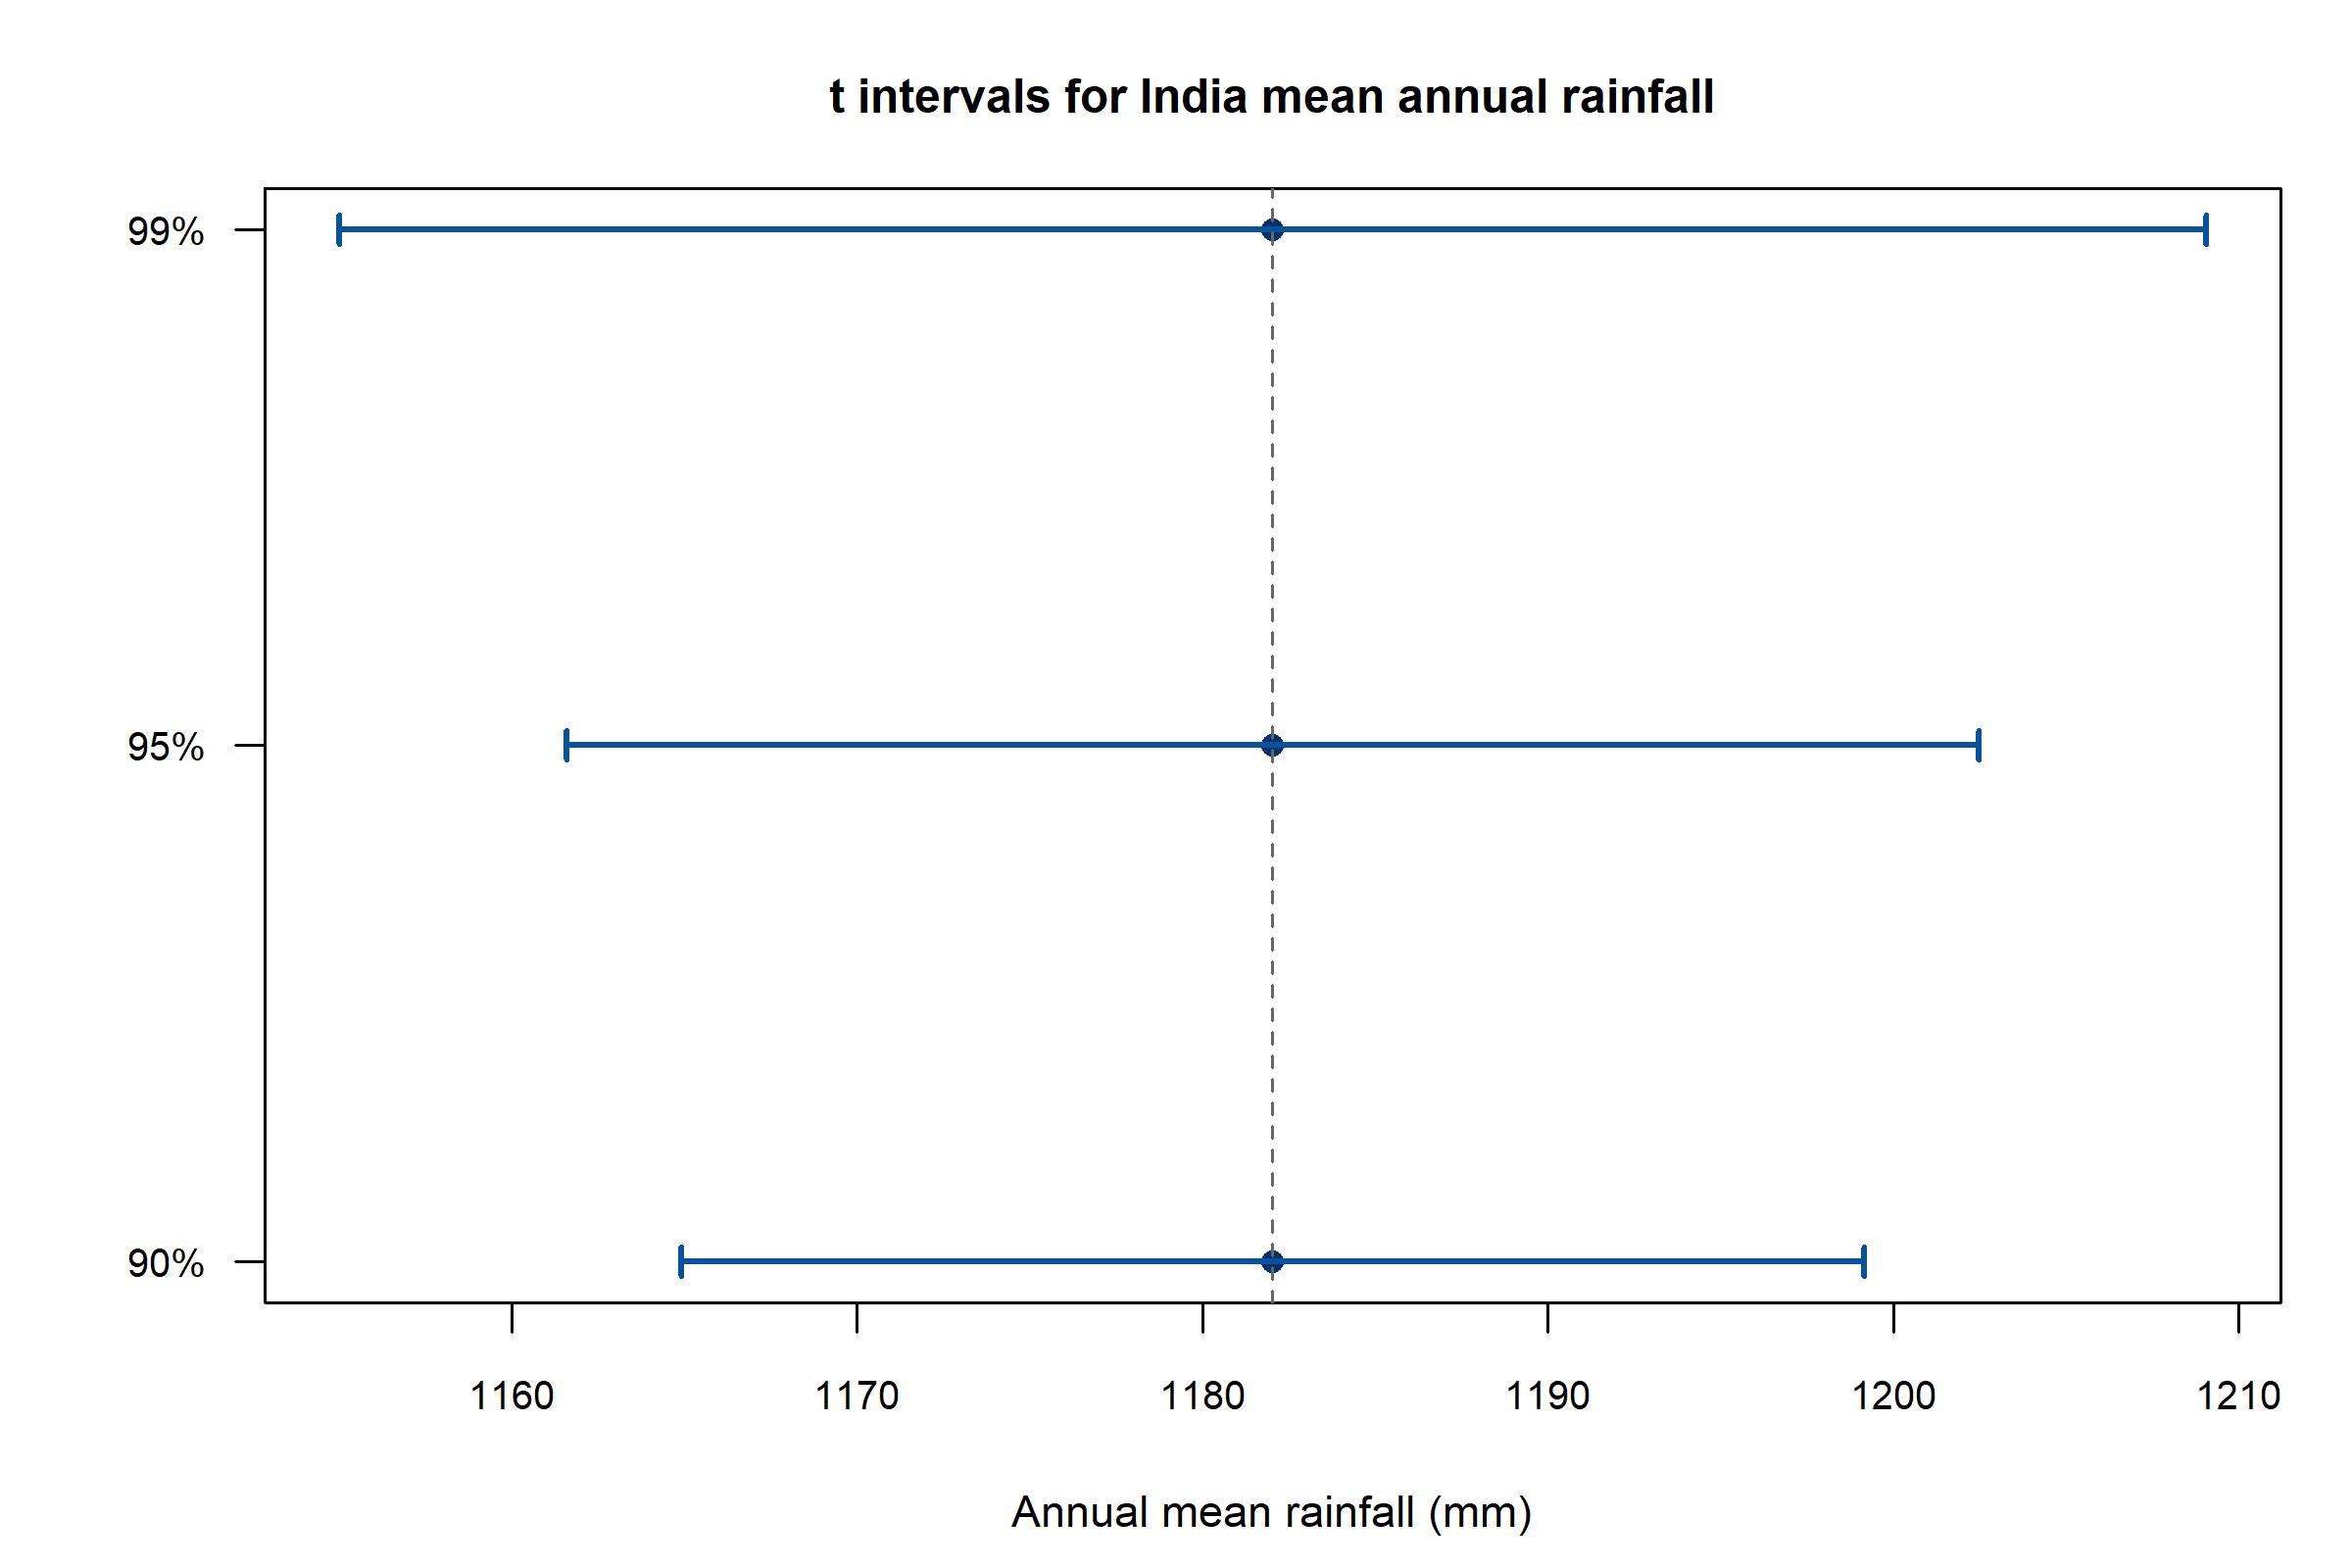
\includegraphics[width=0.92\linewidth]{../graphs/confidence_intervals_mean_compare} 

}

\caption{Figure 10. t intervals for the all-India mean annual rainfall at 90\%, 95\% and 99\% confidence. Higher confidence produces a wider interval.}\label{fig:fig-ci}
\end{figure}

The 90\%, 95\% and 99\% intervals for the annual mean are {[}1164.92,
1199.15{]}, {[}1161.59, 1202.48{]} and {[}1155.00, 1209.07{]} mm. The
95\% interval for mean June--September rainfall is 873.79 to 906.73 mm.

The Wald 95\% interval for the proportion of deficient monsoon years is
0.142 to 0.293, around \(\hat p=\) 0.217. Years are not independent
Bernoulli trials; the interval is a teaching calculation with that
caveat.

\section{Hypothesis testing}\label{hypothesis-testing}

All tests use \(\alpha=0.05\). Failure to reject \(H_0\) does
\textbf{not} prove \(H_0\). \(P\)-values are not posterior probabilities
of hypotheses.

\begin{longtable}[]{@{}
  >{\raggedleft\arraybackslash}p{(\linewidth - 16\tabcolsep) * \real{0.0452}}
  >{\raggedright\arraybackslash}p{(\linewidth - 16\tabcolsep) * \real{0.1921}}
  >{\raggedright\arraybackslash}p{(\linewidth - 16\tabcolsep) * \real{0.3446}}
  >{\raggedright\arraybackslash}p{(\linewidth - 16\tabcolsep) * \real{0.0452}}
  >{\raggedleft\arraybackslash}p{(\linewidth - 16\tabcolsep) * \real{0.0565}}
  >{\raggedleft\arraybackslash}p{(\linewidth - 16\tabcolsep) * \real{0.0508}}
  >{\raggedright\arraybackslash}p{(\linewidth - 16\tabcolsep) * \real{0.0508}}
  >{\raggedright\arraybackslash}p{(\linewidth - 16\tabcolsep) * \real{0.1186}}
  >{\raggedright\arraybackslash}p{(\linewidth - 16\tabcolsep) * \real{0.0960}}@{}}
\caption{Table 8. Hypothesis tests at alpha = 0.05. Full write-ups
follow.}\tabularnewline
\toprule\noalign{}
\begin{minipage}[b]{\linewidth}\raggedleft
test\_id
\end{minipage} & \begin{minipage}[b]{\linewidth}\raggedright
procedure
\end{minipage} & \begin{minipage}[b]{\linewidth}\raggedright
H0
\end{minipage} & \begin{minipage}[b]{\linewidth}\raggedright
n
\end{minipage} & \begin{minipage}[b]{\linewidth}\raggedleft
statistic
\end{minipage} & \begin{minipage}[b]{\linewidth}\raggedleft
df
\end{minipage} & \begin{minipage}[b]{\linewidth}\raggedright
p\_value
\end{minipage} & \begin{minipage}[b]{\linewidth}\raggedright
ci\_95
\end{minipage} & \begin{minipage}[b]{\linewidth}\raggedright
decision
\end{minipage} \\
\midrule\noalign{}
\endfirsthead
\toprule\noalign{}
\begin{minipage}[b]{\linewidth}\raggedleft
test\_id
\end{minipage} & \begin{minipage}[b]{\linewidth}\raggedright
procedure
\end{minipage} & \begin{minipage}[b]{\linewidth}\raggedright
H0
\end{minipage} & \begin{minipage}[b]{\linewidth}\raggedright
n
\end{minipage} & \begin{minipage}[b]{\linewidth}\raggedleft
statistic
\end{minipage} & \begin{minipage}[b]{\linewidth}\raggedleft
df
\end{minipage} & \begin{minipage}[b]{\linewidth}\raggedright
p\_value
\end{minipage} & \begin{minipage}[b]{\linewidth}\raggedright
ci\_95
\end{minipage} & \begin{minipage}[b]{\linewidth}\raggedright
decision
\end{minipage} \\
\midrule\noalign{}
\endhead
\bottomrule\noalign{}
\endlastfoot
1 & One-sample t-test & mu = 1180 mm & 115 & 0.197 & 114.0000 & 0.8441 &
{[}1161.588, 1202.482{]} & Do not reject H0 \\
2 & Wilcoxon signed-rank (one-sample) & median = 1180 mm & 115 &
3420.000 & NA & 0.8136 & {[}1160.850, 1204.150{]} & Do not reject H0 \\
3 & Welch two-sample t-test & mu\_Kerala = mu\_WestRajasthan & 115+115 &
64.768 & 129.0925 & \textless{} 0.0001 & {[}2552.389, 2713.241{]} &
Reject H0 \\
4 & Wilcoxon rank-sum & P(Kerala \textgreater{} Rajasthan) = 0.5 (equal
distributions on a shift) & 115+115 & 13225.000 & NA & \textless{}
0.0001 & see output file & Reject H0 \\
5 & Paired t-test & mu\_(JJAS - OND) = 0 & 115 & 96.377 & 114.0000 &
\textless{} 0.0001 & {[}754.543, 786.213{]} & Reject H0 \\
6 & Wilcoxon signed-rank (paired) & median(JJAS - OND) = 0 & 115 &
6670.000 & NA & \textless{} 0.0001 & {[}755.000, 789.250{]} & Reject
H0 \\
7 & Chi-square goodness-of-fit & p\_JF = p\_MAM = p\_JJAS = p\_OND = 1/4
& 115 & 345.000 & 3.0000 & \textless{} 0.0001 & NA & Reject H0 \\
8 & Chi-square test of independence & period and monsoon category are
independent & 115 & 0.335 & 2.0000 & 0.8456 & NA & Do not reject H0 \\
\end{longtable}

\subsection{\texorpdfstring{One-sample \(t\)-test (all-India annual mean
versus 1180
mm)}{One-sample t-test (all-India annual mean versus 1180 mm)}}\label{one-sample-t-test-all-india-annual-mean-versus-1180-mm}

\textbf{Question.} Is the mean of this area-weighted annual series
different from 1180 mm (a round textbook figure of about 118 cm)?

\textbf{Hypotheses.} \(H_0:\mu=1180\) mm versus \(H_1:\mu\neq 1180\) mm.

\textbf{Method and assumptions.} One-sample \(t\), \(n=115\), df
\(=114\). Shapiro--Wilk \(W=0.9926\), \(p=0.8014\). Independence of
years is approximate.

\textbf{Result.} \(\bar x=\) 1182.03 mm, \(t=\) 0.197, \(p=\) 0.8441,
95\% CI {[}1161.59, 1202.48{]} mm.

\textbf{Decision.} Do not reject \(H_0\).

\textbf{Interpretation.} This historical mean is compatible with 1180
mm. That does not validate every textbook sentence, and it does not say
the true generating mean ``is'' 1180 mm.

Wilcoxon signed-rank against median 1180 mm: \(V=3420\), \(p=\) 0.8136;
same decision.

\subsection{\texorpdfstring{Welch two-sample \(t\)-test (Kerala versus
West
Rajasthan)}{Welch two-sample t-test (Kerala versus West Rajasthan)}}\label{welch-two-sample-t-test-kerala-versus-west-rajasthan}

\textbf{Question.} Do two climatic extremes differ in mean annual
rainfall?

\textbf{Hypotheses.} \(H_0:\mu_K=\mu_R\) versus \(H_1:\mu_K\neq\mu_R\).

\textbf{Design.} Independent samples (different places), complete years
1901--2015, \(n_K=n_R=115\). Variances are unequal (Kerala
\(s^2\approx 1.78\times 10^5\), West Rajasthan
\(s^2\approx 1.18\times 10^4\)), so Welch's \(t\) is used, not Student's
equal-variance \(t\). Shapiro--Wilk \(p=0.046\) (Kerala) and \(p=0.001\)
(West Rajasthan); the rank-sum test is therefore reported as well. An
independent two-sample test would be \textbf{wrong} for two seasons of
the same year.

\textbf{Result.} \(t=\) 64.768, df \(\approx\) 129.1, \(p<\) 0.0001,
95\% CI for \(\mu_K-\mu_R\): 2552.4 to 2713.2 mm.

\textbf{Decision.} Reject \(H_0\). Wilcoxon rank-sum \(W=13225\), \(p<\)
0.0001.

\textbf{Interpretation.} Kerala is wetter by about 2.6 metres per year
on average. That is the climatology of a monsoon coast versus the Thar
margin, not a surprising discovery. The test documents the contrast with
uncertainty.

\subsection{\texorpdfstring{Paired \(t\)-test (June--September versus
October--December)}{Paired t-test (June--September versus October--December)}}\label{paired-t-test-juneseptember-versus-octoberdecember}

\textbf{Question.} Within a year, does southwest-monsoon rainfall differ
from post-monsoon rainfall?

\textbf{Hypotheses.} \(H_0:\mu_{\mathrm{JJAS}-\mathrm{OND}}=0\) versus
\(H_1\neq 0\).

\textbf{Design.} Pairing is required because both seasons belong to the
same year.

\textbf{Assumptions.} Shapiro--Wilk on differences: \(W=0.9856\),
\(p=0.2557\).

\textbf{Result.} \(t=\) 96.377, df \(=114\), \(p<\) 0.0001, 95\% CI
754.5 to 786.2 mm.

\textbf{Decision.} Reject \(H_0\). Paired Wilcoxon \(p<\) 0.0001.

\textbf{Interpretation.} The monsoon exceeds post-monsoon by roughly
three-quarters of a metre in a typical year. This is the definition of a
monsoon climate, confirmed statistically.

\subsection{Chi-square goodness-of-fit (wettest
season)}\label{chi-square-goodness-of-fit-wettest-season}

Raw millimetres were \textbf{not} put into a chi-square test. Each year
was classified by which IMD season had the largest total. Under \(H_0\),
each season has probability \(1/4\), so expected count \(=115/4=28.75\)
(all \(>5\)).

Observed counts: January--February 0, March--May 0, June--September 115,
October--December 0. \(\chi^2=345\), df \(=3\), \(p<\) 0.0001. Reject
\(H_0\). The southwest monsoon was the wettest season in every year of
this national series.

\subsection{\texorpdfstring{Chi-square test of independence (period
\(\times\) monsoon
class)}{Chi-square test of independence (period \textbackslash times monsoon class)}}\label{chi-square-test-of-independence-period-times-monsoon-class}

Years were split at 1958. Monsoon class uses 90\%/110\% of the
\textbf{full-series} June--September mean. \(H_0\): period and class are
independent.

Counts: 1901--1957: 12 deficient, 38 normal, 7 excess; 1958--2015: 13,
36, 9. \(\chi^2=\) 0.34, df \(=2\), \(p=\) 0.8456. Do not reject
\(H_0\). Adjacent years are dependent, so the nominal \(p\)-value is
approximate. This is \textbf{not} a test of climate change.

\section{Correlation and covariance}\label{correlation-and-covariance}

Pearson \(r\) measures linear association; Spearman \(\rho\) measures
monotonic association. Neither is causation. June--September was
\textbf{not} correlated with the annual total, because the monsoon is a
large numerical part of the year (part--whole artefact).

\begin{longtable}[]{@{}
  >{\raggedright\arraybackslash}p{(\linewidth - 16\tabcolsep) * \real{0.0729}}
  >{\raggedright\arraybackslash}p{(\linewidth - 16\tabcolsep) * \real{0.0729}}
  >{\raggedleft\arraybackslash}p{(\linewidth - 16\tabcolsep) * \real{0.1042}}
  >{\raggedleft\arraybackslash}p{(\linewidth - 16\tabcolsep) * \real{0.1042}}
  >{\raggedleft\arraybackslash}p{(\linewidth - 16\tabcolsep) * \real{0.1771}}
  >{\raggedleft\arraybackslash}p{(\linewidth - 16\tabcolsep) * \real{0.1771}}
  >{\raggedleft\arraybackslash}p{(\linewidth - 16\tabcolsep) * \real{0.1354}}
  >{\raggedleft\arraybackslash}p{(\linewidth - 16\tabcolsep) * \real{0.1146}}
  >{\raggedleft\arraybackslash}p{(\linewidth - 16\tabcolsep) * \real{0.0417}}@{}}
\caption{Table 9. Pairwise season correlations, all-India, 1901--2015.
Annual totals are omitted (part--whole).}\tabularnewline
\toprule\noalign{}
\begin{minipage}[b]{\linewidth}\raggedright
var\_x
\end{minipage} & \begin{minipage}[b]{\linewidth}\raggedright
var\_y
\end{minipage} & \begin{minipage}[b]{\linewidth}\raggedleft
pearson\_r
\end{minipage} & \begin{minipage}[b]{\linewidth}\raggedleft
pearson\_p
\end{minipage} & \begin{minipage}[b]{\linewidth}\raggedleft
pearson\_ci\_lower
\end{minipage} & \begin{minipage}[b]{\linewidth}\raggedleft
pearson\_ci\_upper
\end{minipage} & \begin{minipage}[b]{\linewidth}\raggedleft
spearman\_rho
\end{minipage} & \begin{minipage}[b]{\linewidth}\raggedleft
spearman\_p
\end{minipage} & \begin{minipage}[b]{\linewidth}\raggedleft
n
\end{minipage} \\
\midrule\noalign{}
\endfirsthead
\toprule\noalign{}
\begin{minipage}[b]{\linewidth}\raggedright
var\_x
\end{minipage} & \begin{minipage}[b]{\linewidth}\raggedright
var\_y
\end{minipage} & \begin{minipage}[b]{\linewidth}\raggedleft
pearson\_r
\end{minipage} & \begin{minipage}[b]{\linewidth}\raggedleft
pearson\_p
\end{minipage} & \begin{minipage}[b]{\linewidth}\raggedleft
pearson\_ci\_lower
\end{minipage} & \begin{minipage}[b]{\linewidth}\raggedleft
pearson\_ci\_upper
\end{minipage} & \begin{minipage}[b]{\linewidth}\raggedleft
spearman\_rho
\end{minipage} & \begin{minipage}[b]{\linewidth}\raggedleft
spearman\_p
\end{minipage} & \begin{minipage}[b]{\linewidth}\raggedleft
n
\end{minipage} \\
\midrule\noalign{}
\endhead
\bottomrule\noalign{}
\endlastfoot
JanFeb & MarMay & 0.003 & 0.9728 & -0.180 & 0.186 & 0.014 & 0.8782 &
115 \\
JanFeb & JunSep & 0.143 & 0.1281 & -0.041 & 0.318 & 0.130 & 0.1677 &
115 \\
JanFeb & OctDec & -0.060 & 0.5261 & -0.240 & 0.125 & -0.055 & 0.5618 &
115 \\
MarMay & JunSep & 0.104 & 0.2671 & -0.080 & 0.282 & 0.082 & 0.3829 &
115 \\
MarMay & OctDec & 0.074 & 0.4327 & -0.111 & 0.254 & 0.068 & 0.4711 &
115 \\
JunSep & OctDec & 0.287 & 0.0019 & 0.109 & 0.446 & 0.224 & 0.0161 &
115 \\
\end{longtable}

\begin{figure}

{\centering 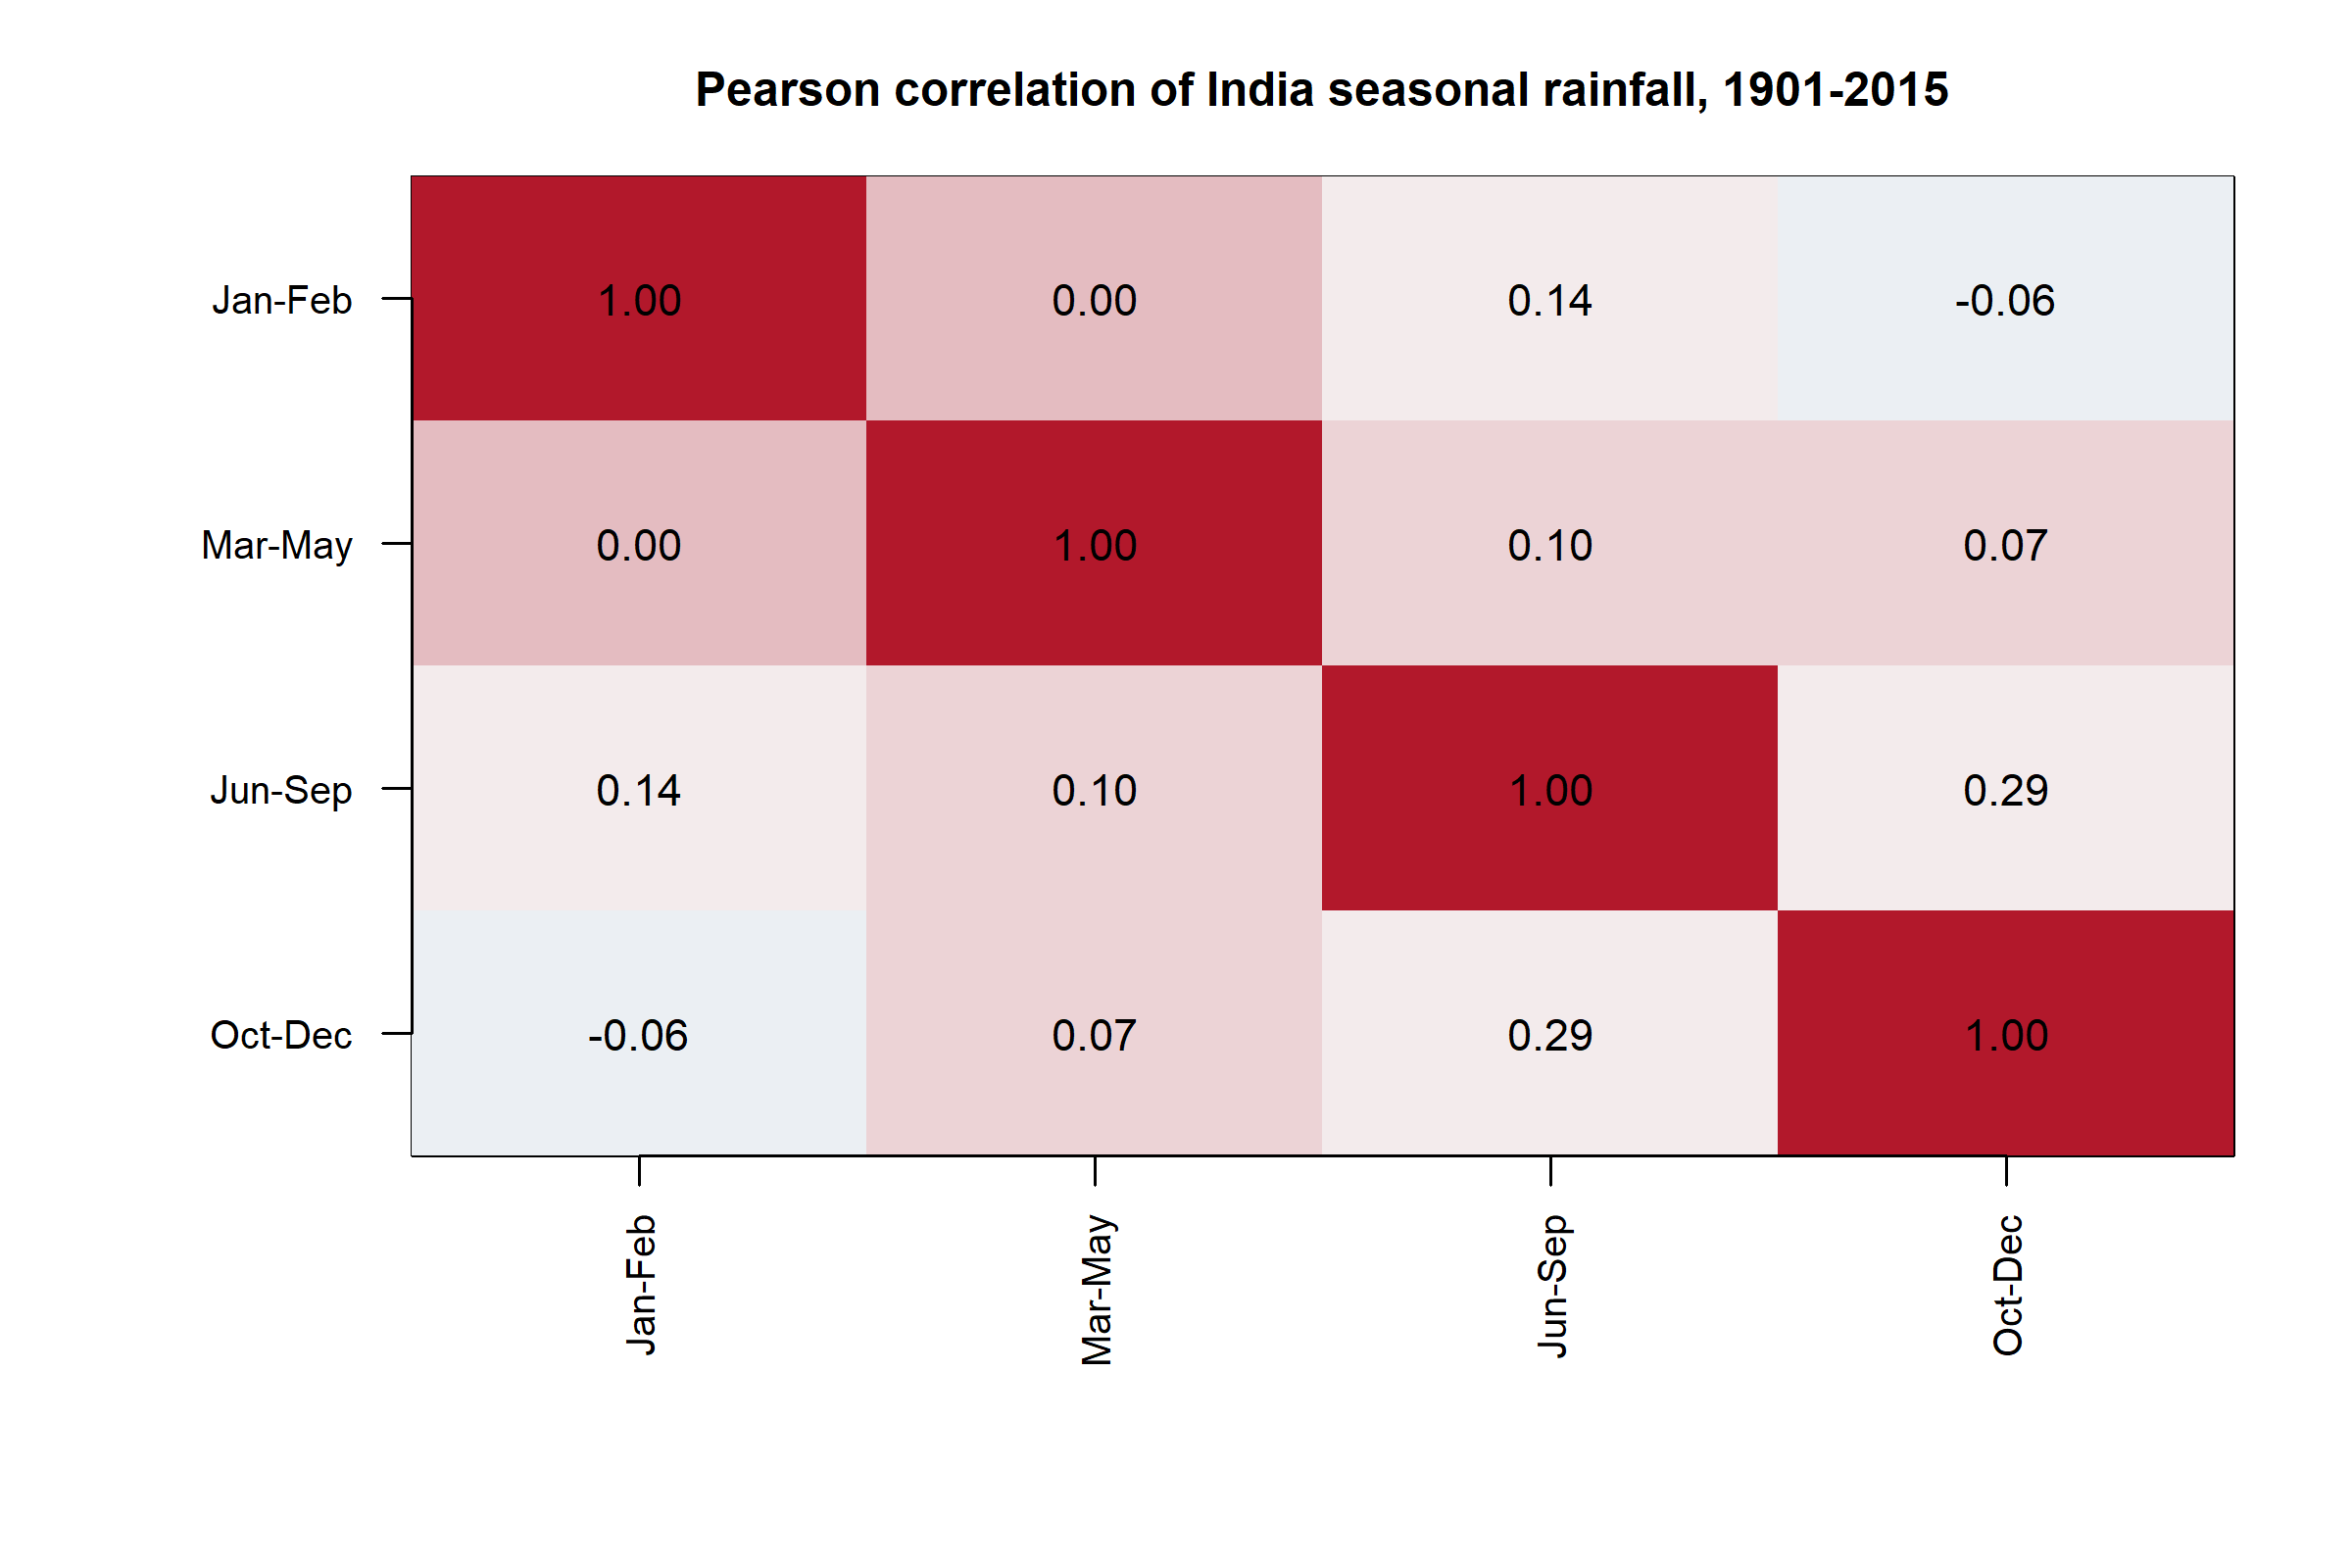
\includegraphics[width=0.92\linewidth]{../graphs/seasonal_correlation_heatmap} 

}

\caption{Figure 11. Pearson correlation heatmap of the four IMD seasonal totals, all-India, 1901–2015.}\label{fig:fig-heat}
\end{figure}

\begin{figure}

{\centering 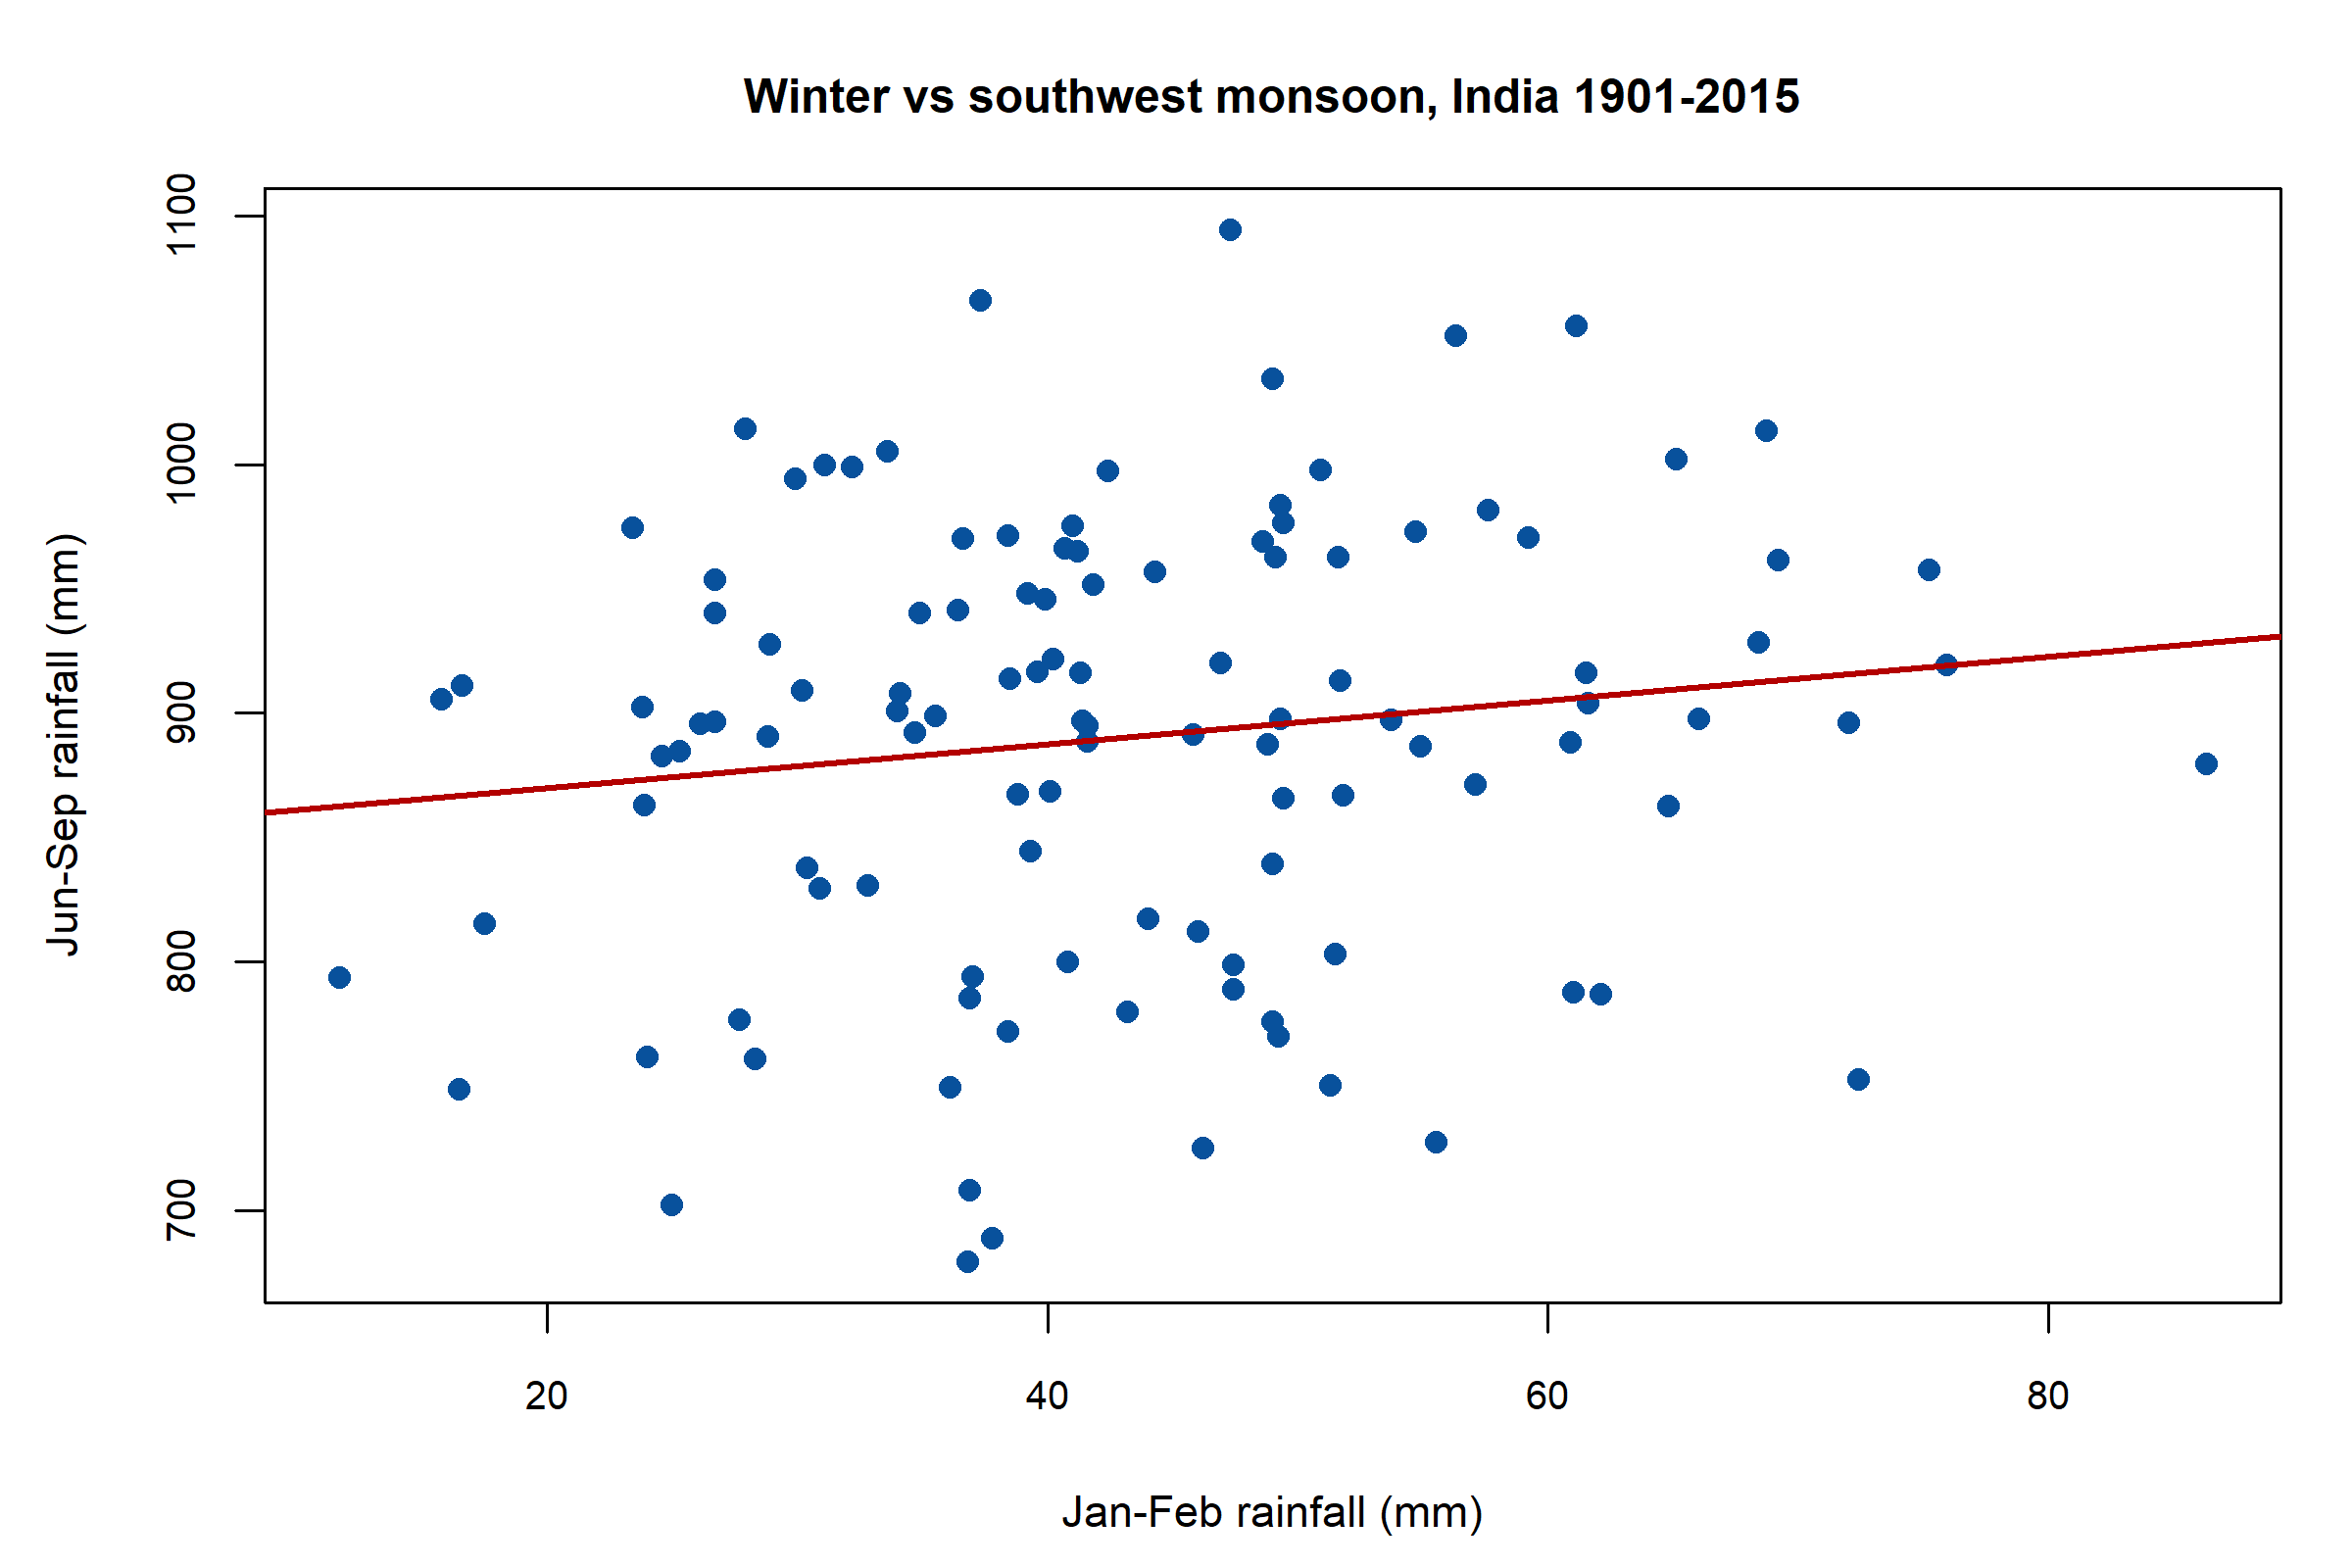
\includegraphics[width=0.92\linewidth]{../graphs/scatter_winter_vs_monsoon} 

}

\caption{Figure 12. January–February versus June–September rainfall (mm). The line is a descriptive OLS fit, not a causal model.}\label{fig:fig-scatter-wm}
\end{figure}

Winter versus monsoon: Pearson \(r=\) 0.143, \(p=\) 0.1281, 95\% CI
\(-0.041\) to \(0.318\). The interval includes 0; there is no
significant linear association in this record. Spearman \(\rho=\) 0.130,
\(p=\) 0.1677.

The only clearly significant seasonal pair is June--September with
October--December: \(r=\) 0.287, \(p=\) 0.0019. That is still
association (wet years can be wet in both seasons), not a claim that the
monsoon \emph{causes} post-monsoon rain.

Year versus annual rainfall: \(r=\) -0.089, \(p=\) 0.3423. No
significant linear time association; see Section 18.

\section{Simple and multiple
regression}\label{simple-and-multiple-regression}

\subsection{Model 1. Annual rainfall on
year}\label{model-1.-annual-rainfall-on-year}

\[
\mathrm{ANNUAL}_i = \beta_0 + \beta_1\,\mathrm{YEAR}_i + \varepsilon_i.
\]

Fitted equation (OLS): \[
\widehat{\mathrm{ANNUAL}} = 1762.9 - 0.2967\times\mathrm{YEAR}.
\]

Slope \(\hat\beta_1=\) -0.2967 mm year\(^{-1}\), SE 0.3110, \(t=\)
-0.954, \(p=\) 0.3423, 95\% CI -0.9129 to 0.3196 mm year\(^{-1}\).

\(R^2=\) 0.0080 (adjusted \(R^2=\) -0.0008): year explains well under
1\% of annual variance. Overall \(F=\) 0.910 on 1 and 113 df, \(p=\)
0.3423.

\textbf{Diagnostics.} Residual Shapiro--Wilk \(p=\) 0.8300; screen of
\(e^2\) on fitted values \(p=\) 0.2430; Durbin--Watson \(d=\) 1.742;
lag-1 residual correlation \(p=\) 0.2098. Cook's distance exceeds
\(4/n\) in 8 years; those years were \textbf{not} deleted. Residual
lag-1 is not significant, but the ACF of the \emph{series} (Section 18)
still shows lag-2 structure, so OLS inference remains an approximation.

\begin{figure}

{\centering 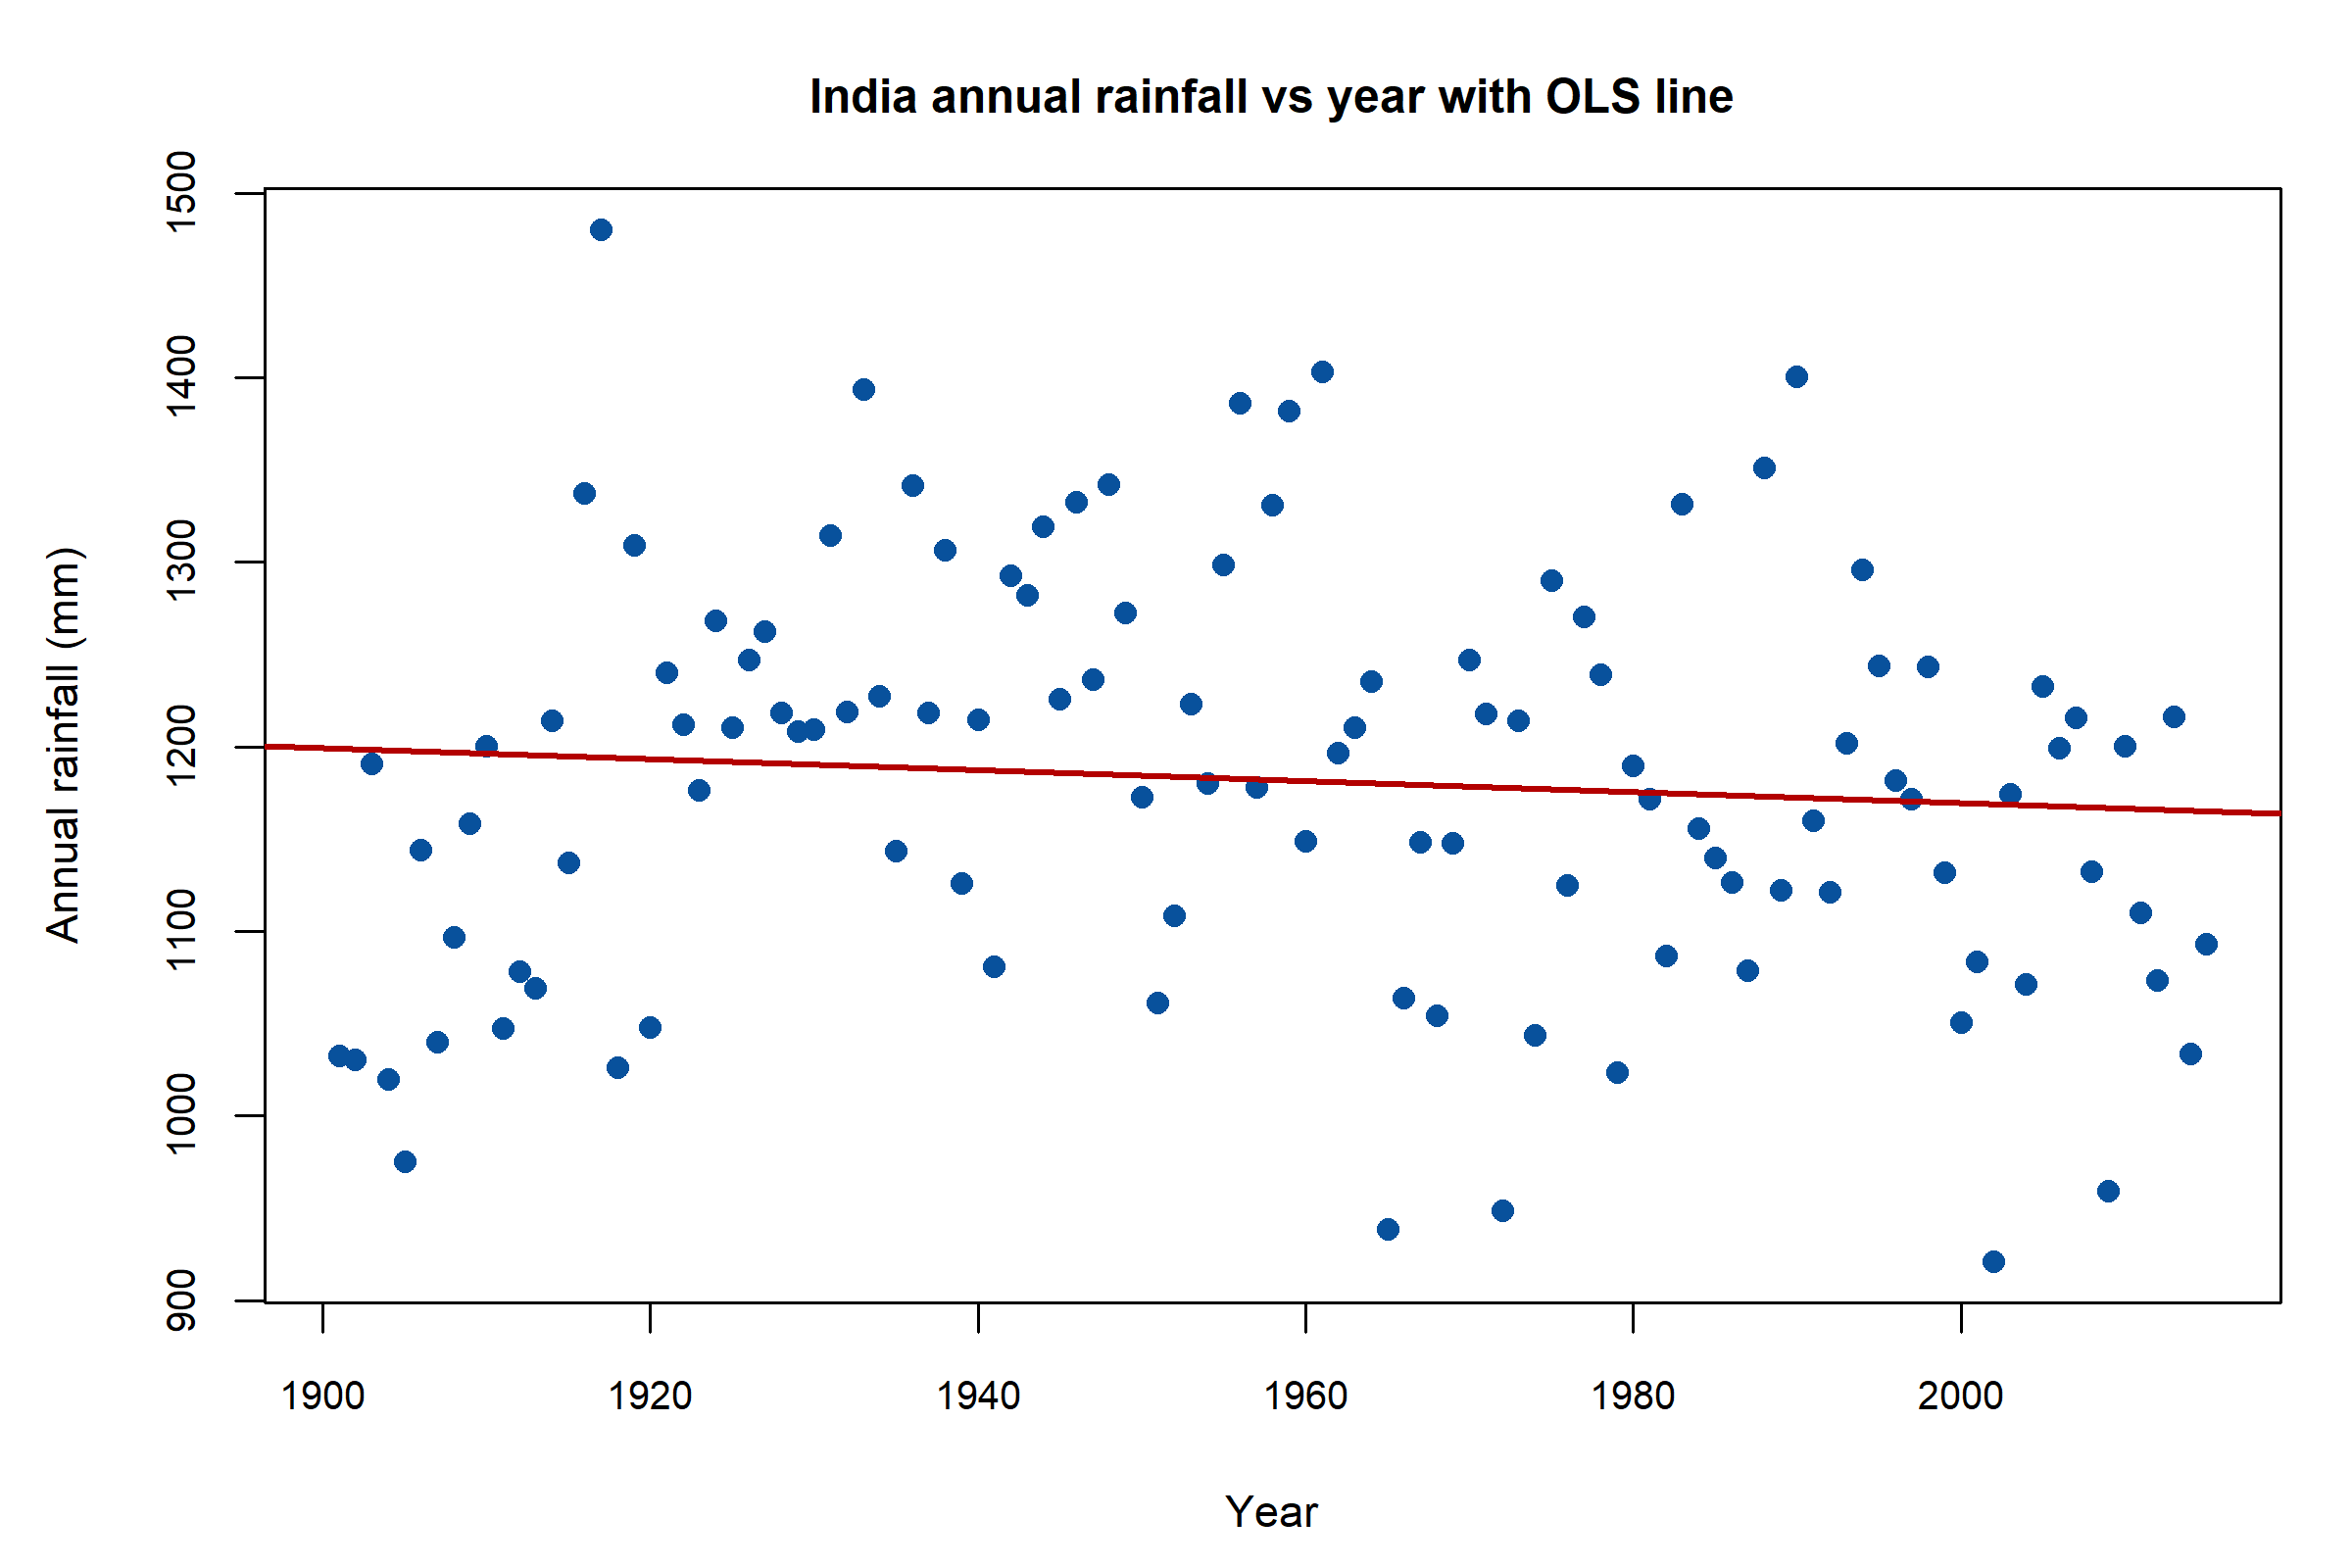
\includegraphics[width=0.92\linewidth]{../graphs/regression_annual_vs_year} 

}

\caption{Figure 13. All-India annual rainfall (mm) versus year with the OLS line. The line is a weak descriptive summary; R-squared is 0.008.}\label{fig:fig-reg}
\end{figure}

\begin{figure}

{\centering 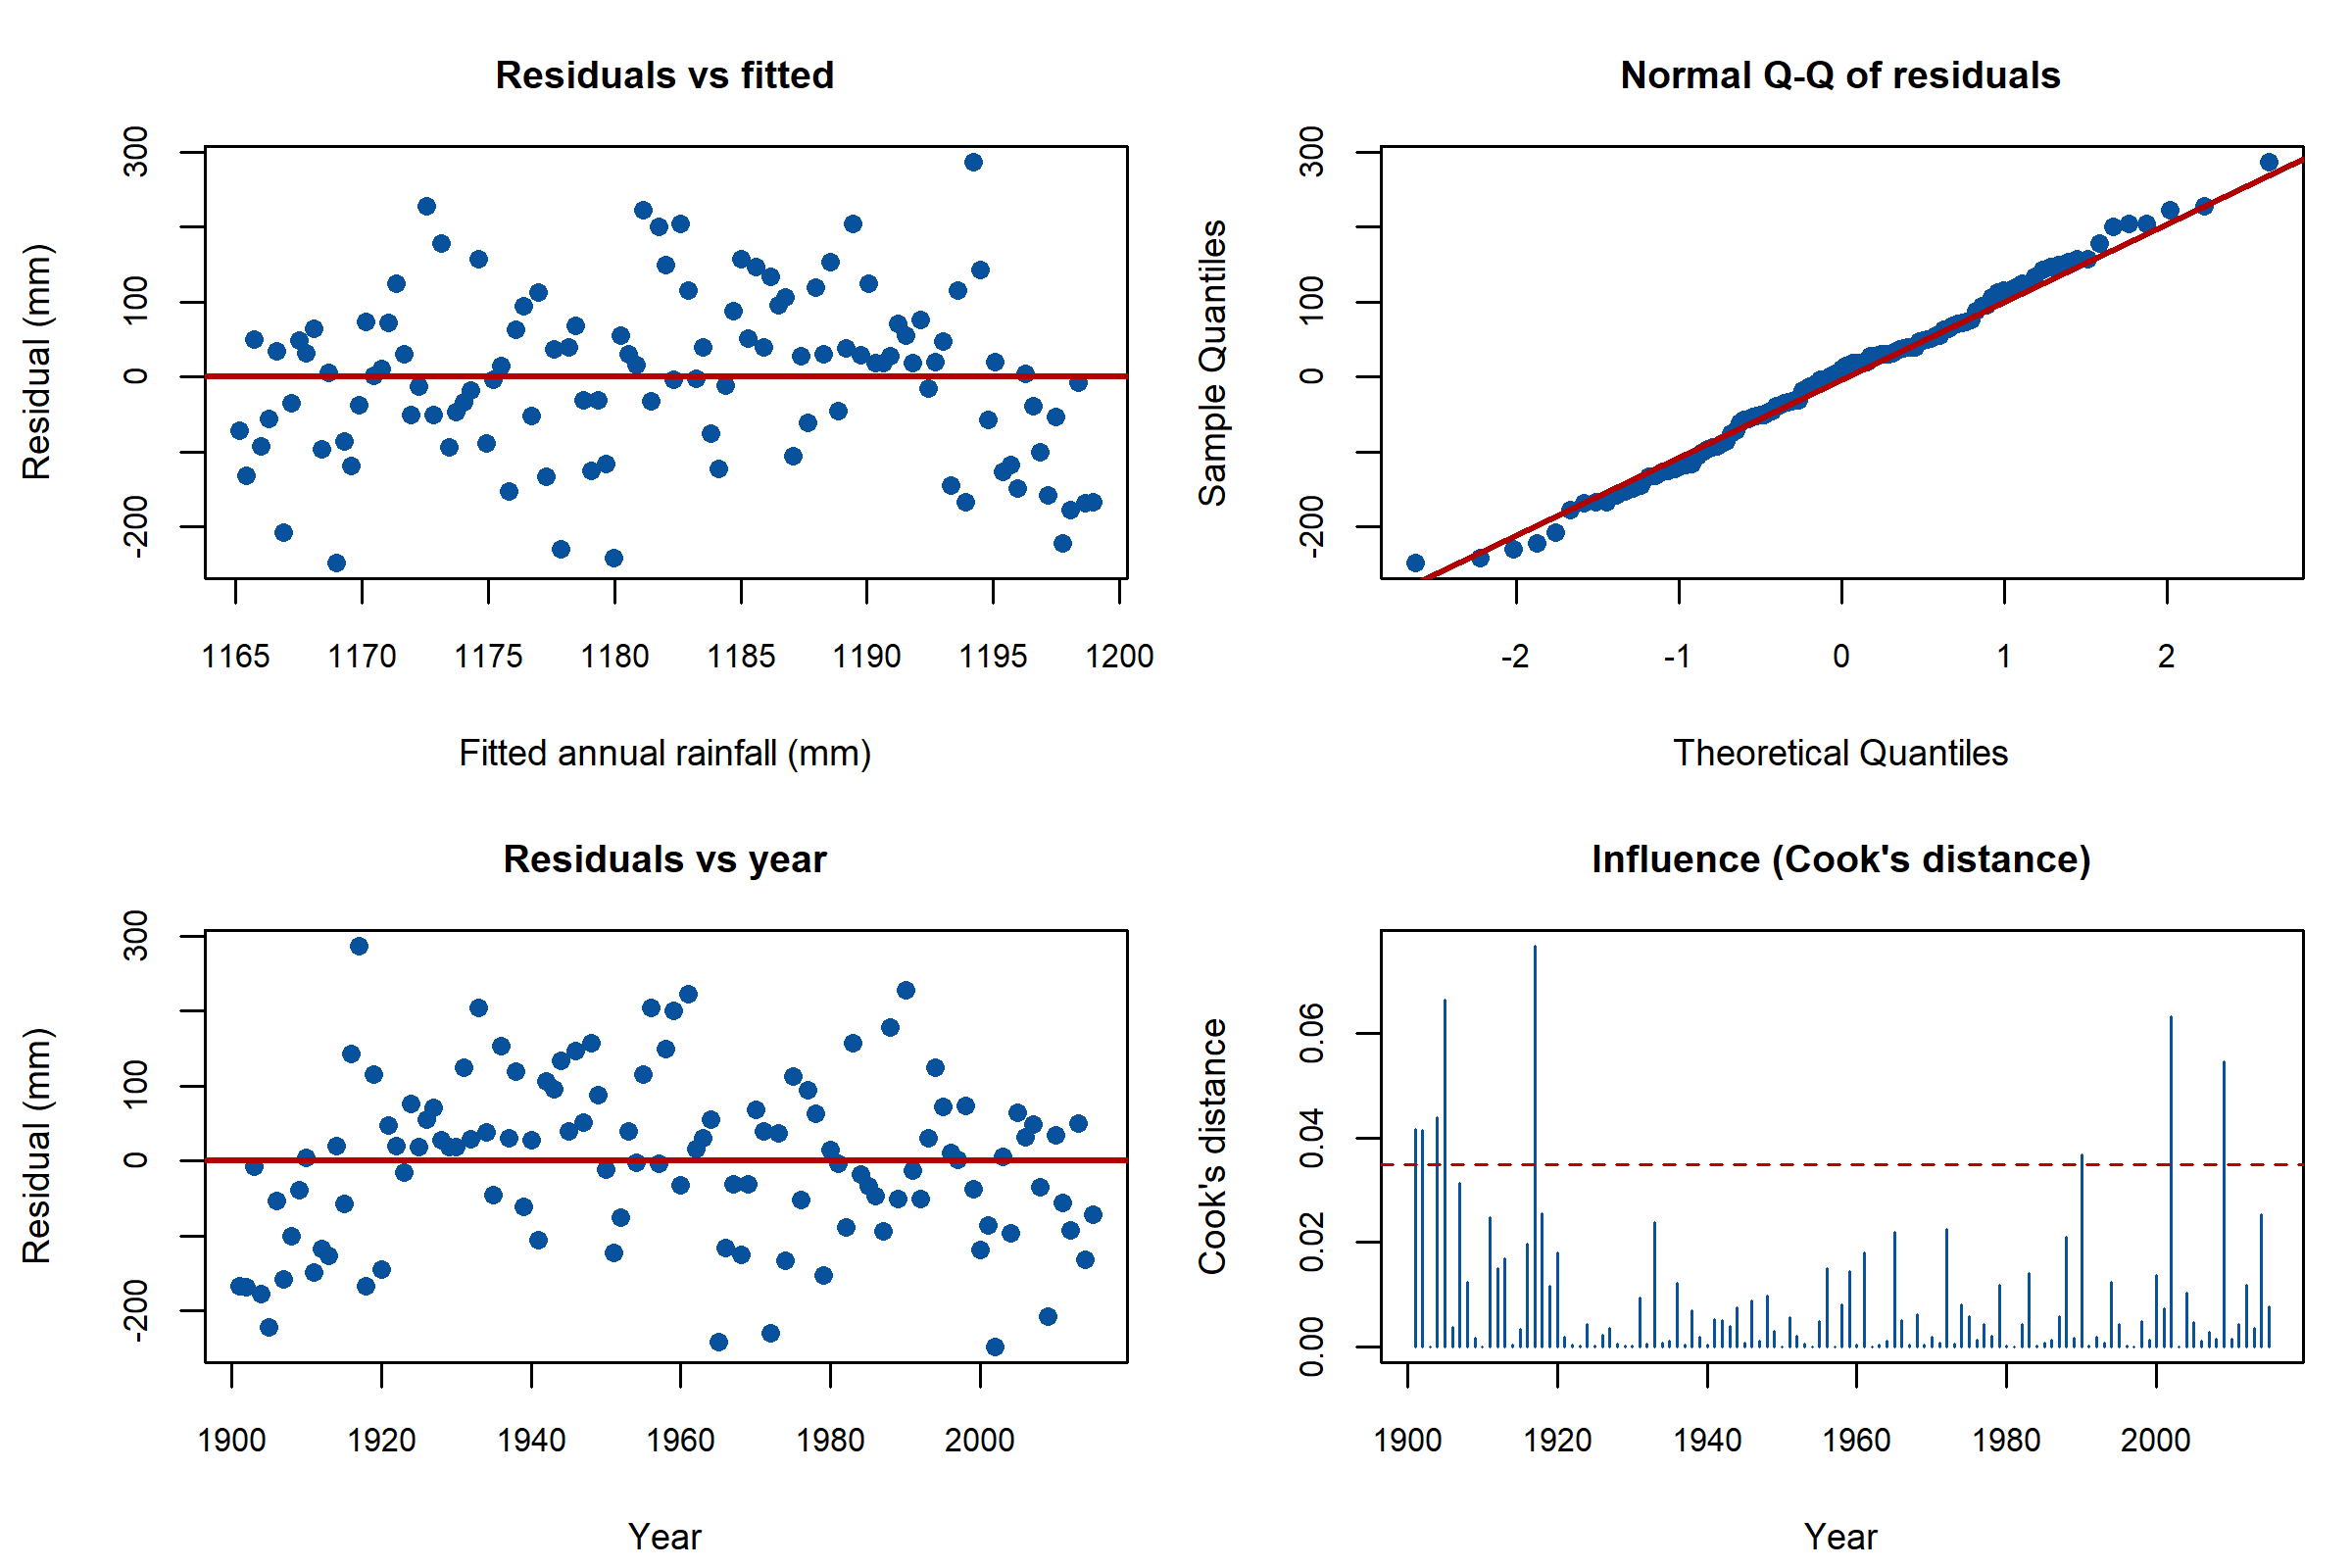
\includegraphics[width=0.92\linewidth]{../graphs/regression_residual_diagnostics} 

}

\caption{Figure 14. OLS residual diagnostics for annual rainfall on year: residuals versus fitted, normal Q–Q, residuals versus year, and Cook's distance.}\label{fig:fig-resid}
\end{figure}

\textbf{Interpretation.} There is no statistically significant linear
decline or rise in all-India annual rainfall in this OLS model. The
fitted slope of about \(-0.30\) mm year\(^{-1}\) would be only about
\(-34\) mm over 115 years, well within year-to-year noise of SD 110.69
mm. This is \textbf{not} a climate-change attribution.

\subsection{Model 2. Monsoon on year and
winter}\label{model-2.-monsoon-on-year-and-winter}

\[
\mathrm{JunSep}_i = \beta_0 + \beta_1\,\mathrm{YEAR}_i + \beta_2\,\mathrm{JanFeb}_i + \varepsilon_i.
\]

Winter is a \textbf{different season}, not a subset of June--September.
No extra predictors were added to inflate \(R^2\).

\(R^2=\) 0.0242, adjusted \(R^2=\) 0.0068, \(F=\) 1.390 (\(p=\) 0.2534).
Year coefficient \(p=\) 0.5079; January--February coefficient
\(\hat\beta_2=\) 0.816 (SE 0.583, \(p=\) 0.1643). Durbin--Watson \(d=\)
1.865.

The multiple regression does not detect a useful linear link from winter
rain or year to all-India monsoon totals in this sample.

\section{ANOVA and regional
comparison}\label{anova-and-regional-comparison}

Regional means use complete-month years in 1901--2015. Equal-weighted
averages of subdivisions are \textbf{not} the national area-weighted
series. Different climates are expected: a significant ANOVA is largely
a confirmation of geography.

Six subdivisions were compared on a balanced window of 114 common years:
Kerala, Coastal Karnataka, Gangetic West Bengal, Tamil Nadu, Punjab and
West Rajasthan.

\begin{longtable}[]{@{}
  >{\raggedright\arraybackslash}p{(\linewidth - 12\tabcolsep) * \real{0.3333}}
  >{\raggedleft\arraybackslash}p{(\linewidth - 12\tabcolsep) * \real{0.1190}}
  >{\raggedleft\arraybackslash}p{(\linewidth - 12\tabcolsep) * \real{0.0476}}
  >{\raggedleft\arraybackslash}p{(\linewidth - 12\tabcolsep) * \real{0.0833}}
  >{\raggedleft\arraybackslash}p{(\linewidth - 12\tabcolsep) * \real{0.0952}}
  >{\raggedleft\arraybackslash}p{(\linewidth - 12\tabcolsep) * \real{0.2024}}
  >{\raggedleft\arraybackslash}p{(\linewidth - 12\tabcolsep) * \real{0.1190}}@{}}
\caption{Table 10. Tests of equal mean annual rainfall among six
subdivisions (balanced common years).}\tabularnewline
\toprule\noalign{}
\begin{minipage}[b]{\linewidth}\raggedright
test
\end{minipage} & \begin{minipage}[b]{\linewidth}\raggedleft
statistic
\end{minipage} & \begin{minipage}[b]{\linewidth}\raggedleft
df1
\end{minipage} & \begin{minipage}[b]{\linewidth}\raggedleft
df2
\end{minipage} & \begin{minipage}[b]{\linewidth}\raggedleft
p\_value
\end{minipage} & \begin{minipage}[b]{\linewidth}\raggedleft
n\_years\_balanced
\end{minipage} & \begin{minipage}[b]{\linewidth}\raggedleft
n\_regions
\end{minipage} \\
\midrule\noalign{}
\endfirsthead
\toprule\noalign{}
\begin{minipage}[b]{\linewidth}\raggedright
test
\end{minipage} & \begin{minipage}[b]{\linewidth}\raggedleft
statistic
\end{minipage} & \begin{minipage}[b]{\linewidth}\raggedleft
df1
\end{minipage} & \begin{minipage}[b]{\linewidth}\raggedleft
df2
\end{minipage} & \begin{minipage}[b]{\linewidth}\raggedleft
p\_value
\end{minipage} & \begin{minipage}[b]{\linewidth}\raggedleft
n\_years\_balanced
\end{minipage} & \begin{minipage}[b]{\linewidth}\raggedleft
n\_regions
\end{minipage} \\
\midrule\noalign{}
\endhead
\bottomrule\noalign{}
\endlastfoot
Classical one-way ANOVA & 2134.70 & 5 & 678.00 & 0 & 114 & 6 \\
Welch one-way ANOVA & 1988.47 & 5 & 307.23 & 0 & 114 & 6 \\
Kruskal-Wallis & 639.91 & NA & 5.00 & 0 & 114 & 6 \\
Fligner-Killeen (variances) & 202.21 & 5 & NA & 0 & 114 & 6 \\
\end{longtable}

Fligner--Killeen rejects equal variances (\(\chi^2=\) 202.2, \(p<\)
0.0001). Classical ANOVA \(F=\) 2134.7 is therefore not the primary
result. \textbf{Welch ANOVA} \(F=\) 1988.5, \(p<\) 0.0001.
Kruskal--Wallis \(\chi^2=\) 639.9, df \(=5\), \(p<\) 0.0001. Reject
equal regional means.

Bonferroni-adjusted pairwise Welch tests reject every pair among the six
regions at \(\alpha=0.05\) (all adjusted \(p<\) 0.0001; see
\texttt{anova\_pairwise\_welch\_bonferroni.csv}). Tukey HSD, which
assumes equal variances, is saved but should be treated cautiously given
Fligner's result. Wilcoxon pairwise tests agree on the same qualitative
separations.

\begin{figure}

{\centering 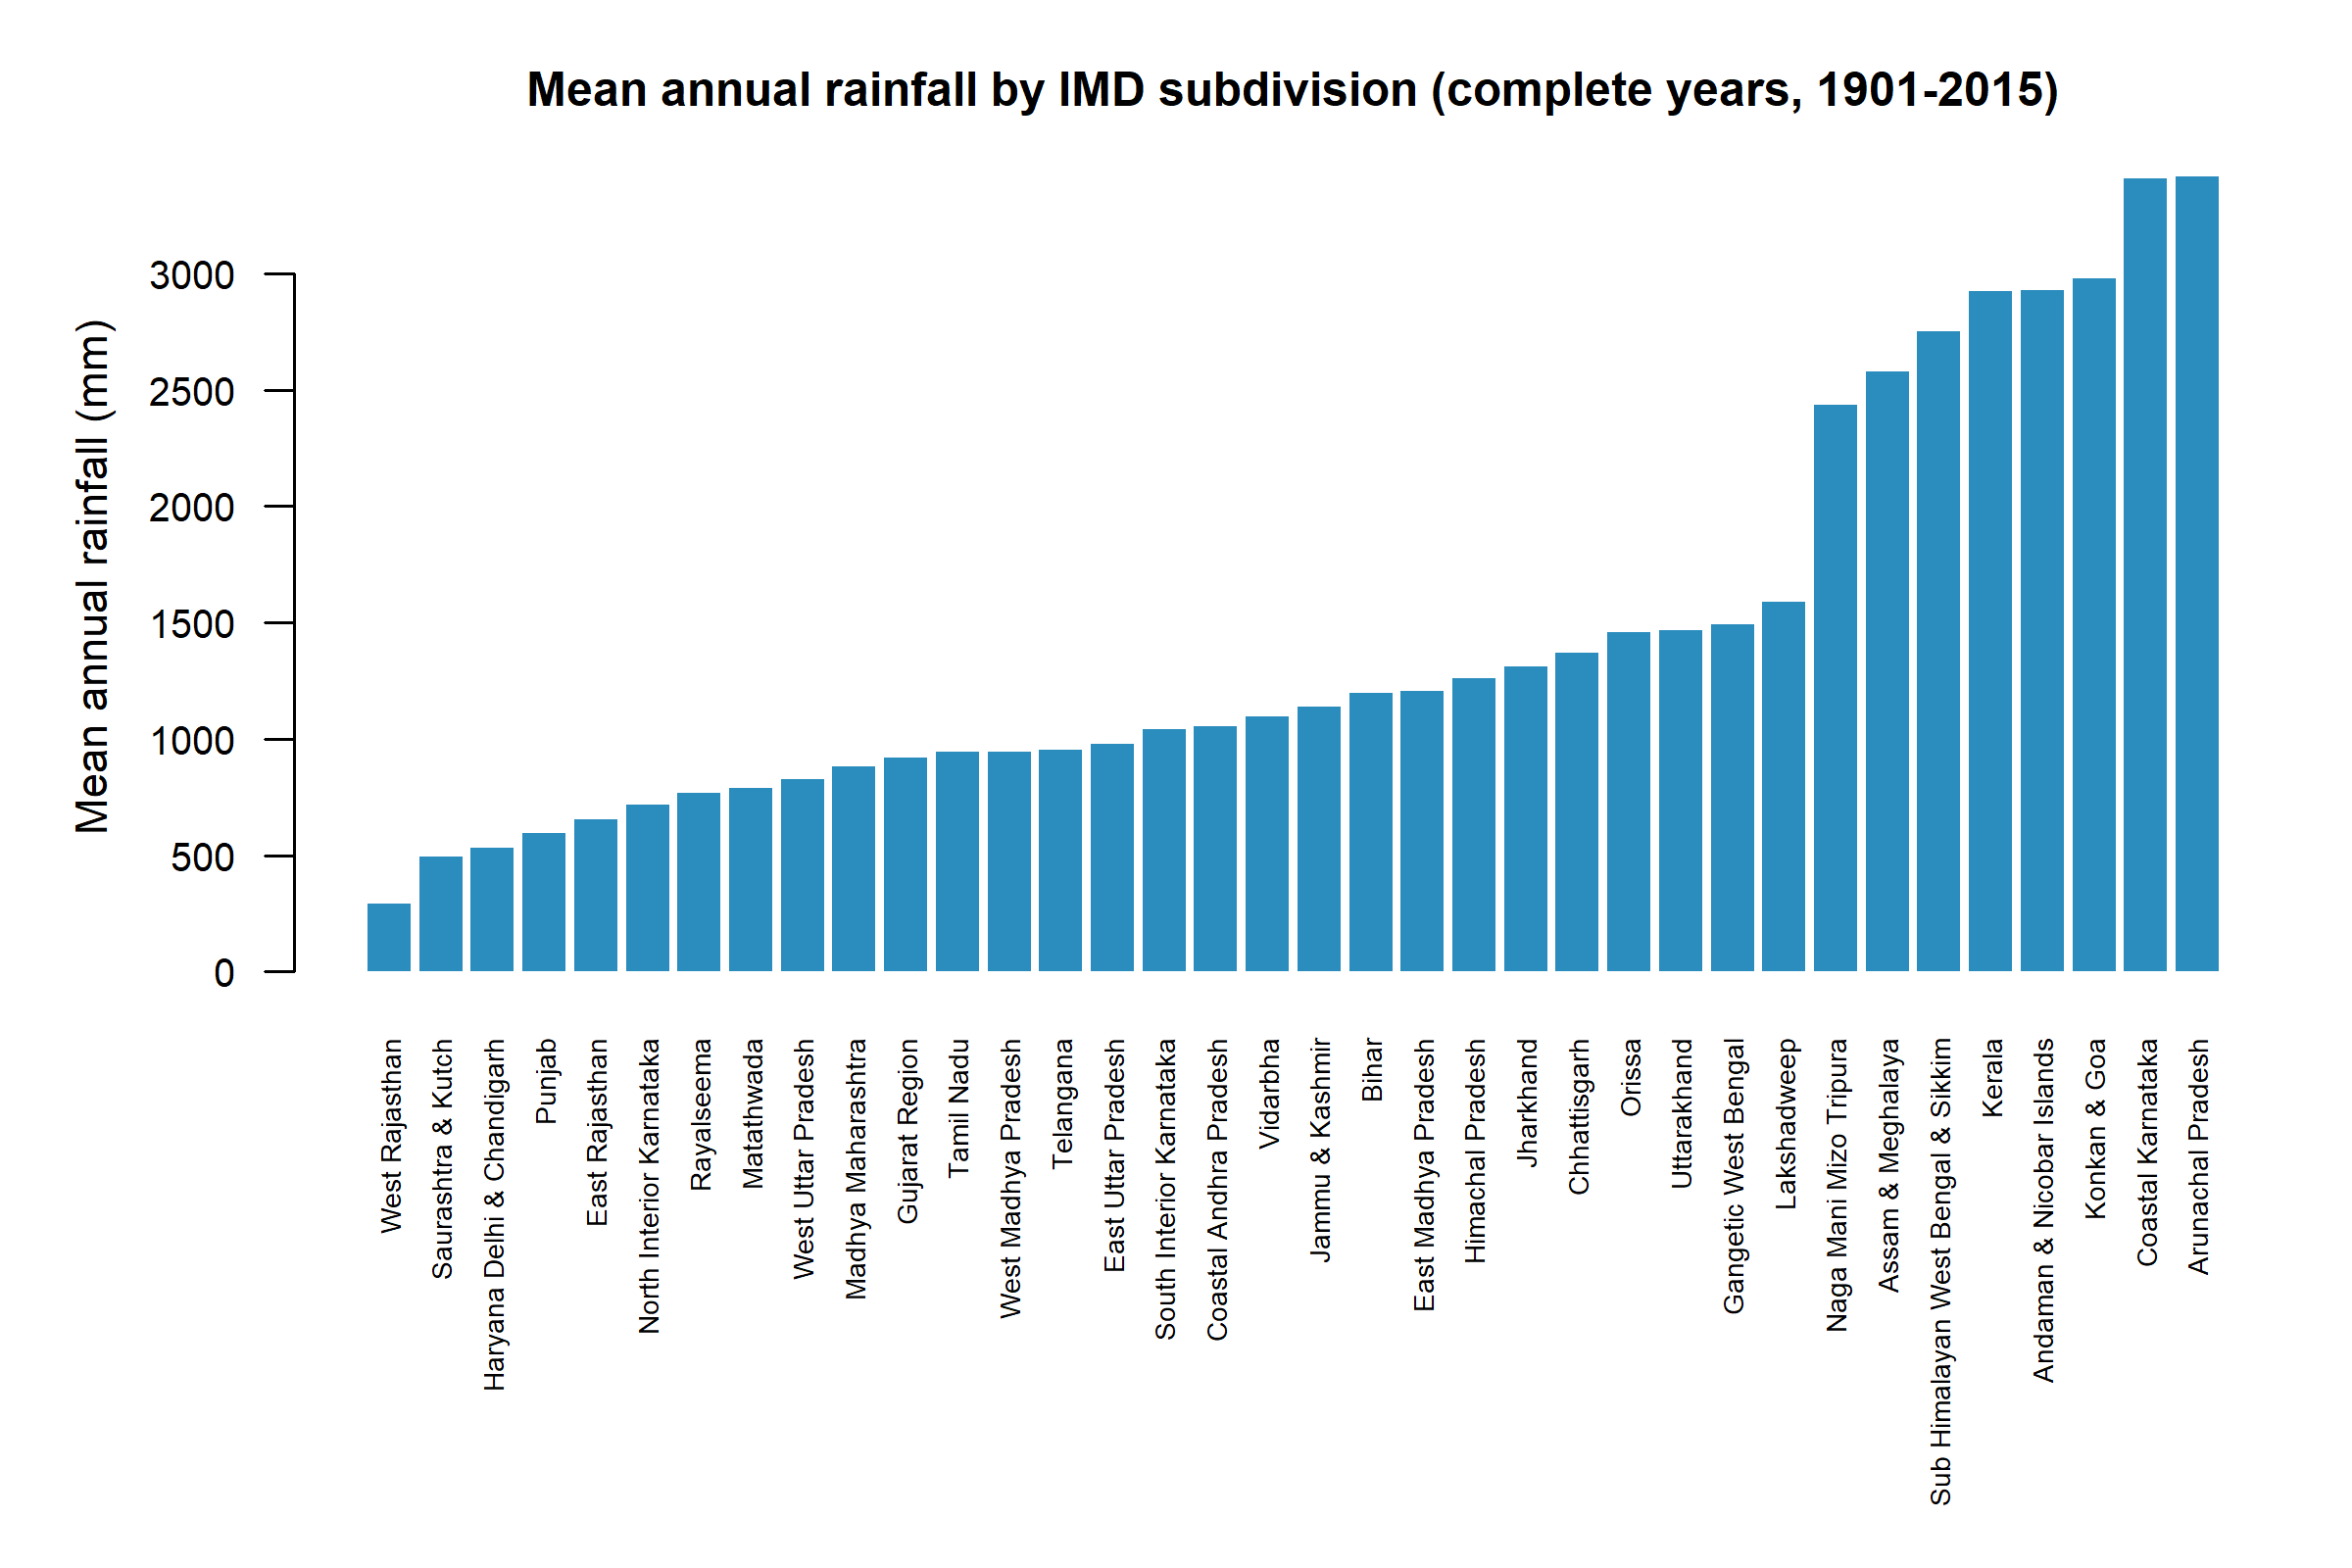
\includegraphics[width=0.92\linewidth]{../graphs/regional_mean_annual_rainfall} 

}

\caption{Figure 15. Mean annual rainfall (mm) by IMD subdivision, complete years 1901–2015.}\label{fig:fig-regmean}
\end{figure}

\begin{figure}

{\centering 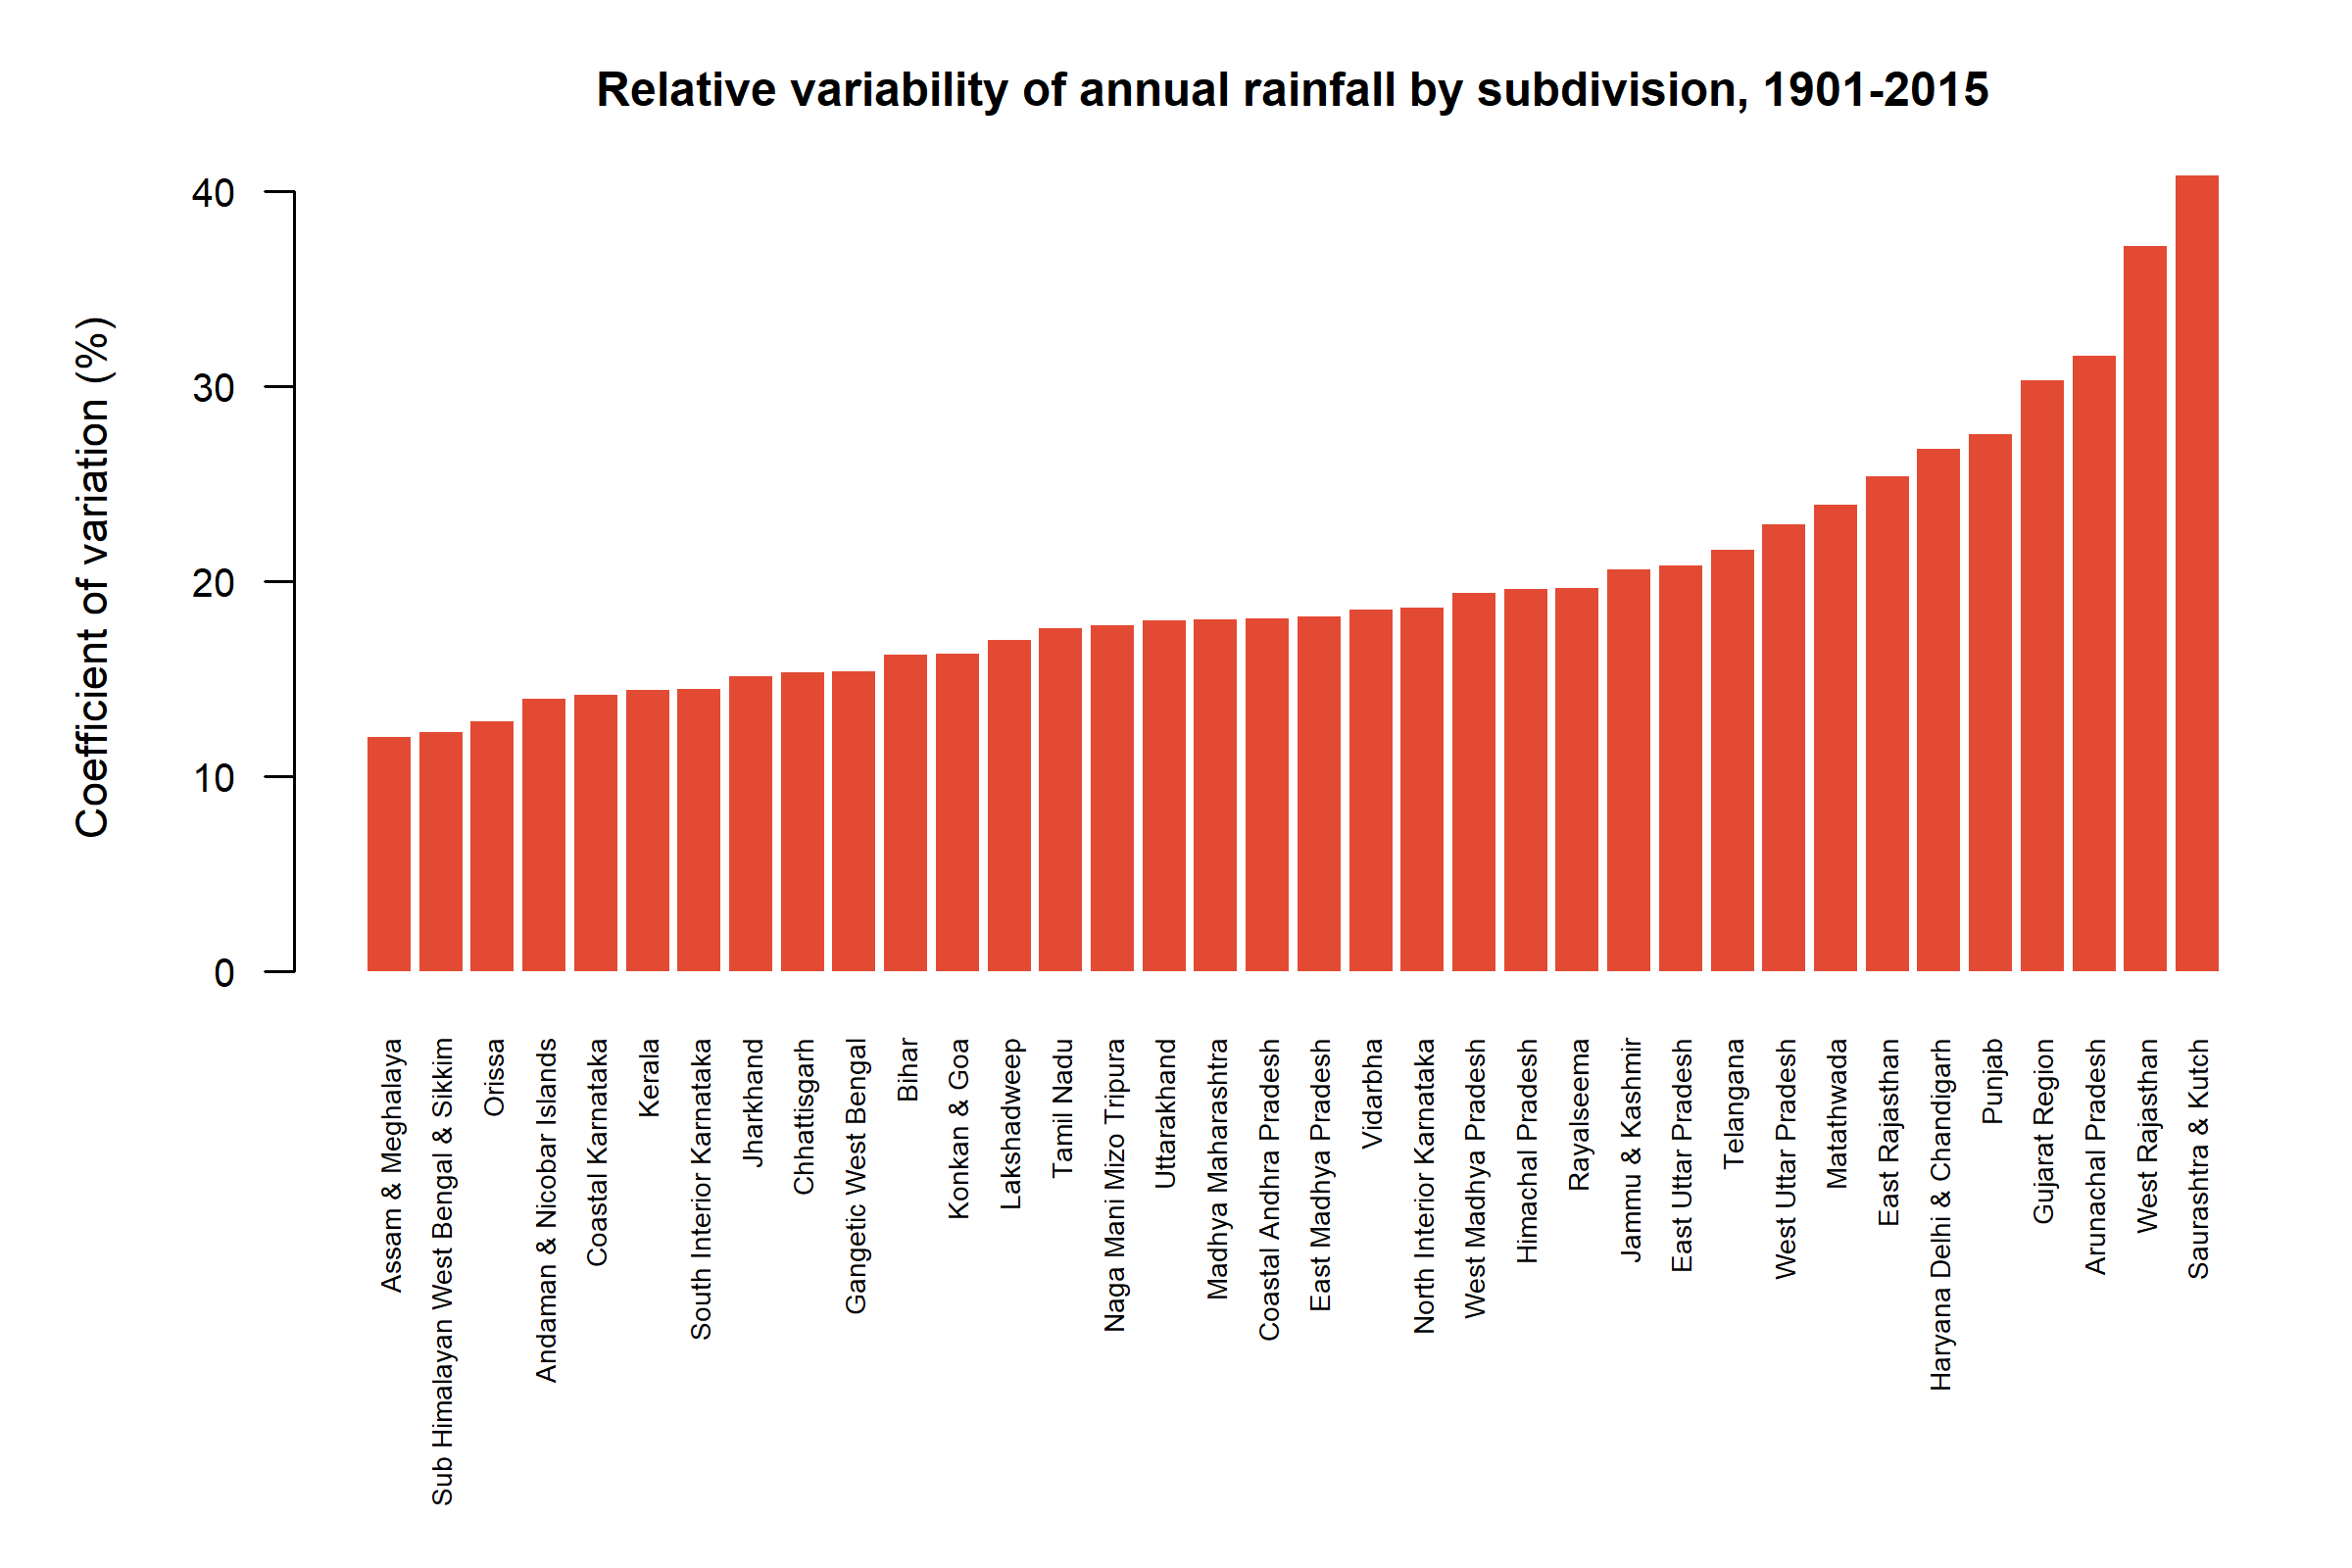
\includegraphics[width=0.92\linewidth]{../graphs/regional_cv_annual_rainfall} 

}

\caption{Figure 16. Coefficient of variation (\%) of annual rainfall by subdivision, 1901–2015. Arid subdivisions are more variable relative to their mean.}\label{fig:fig-regcv}
\end{figure}

\begin{figure}

{\centering 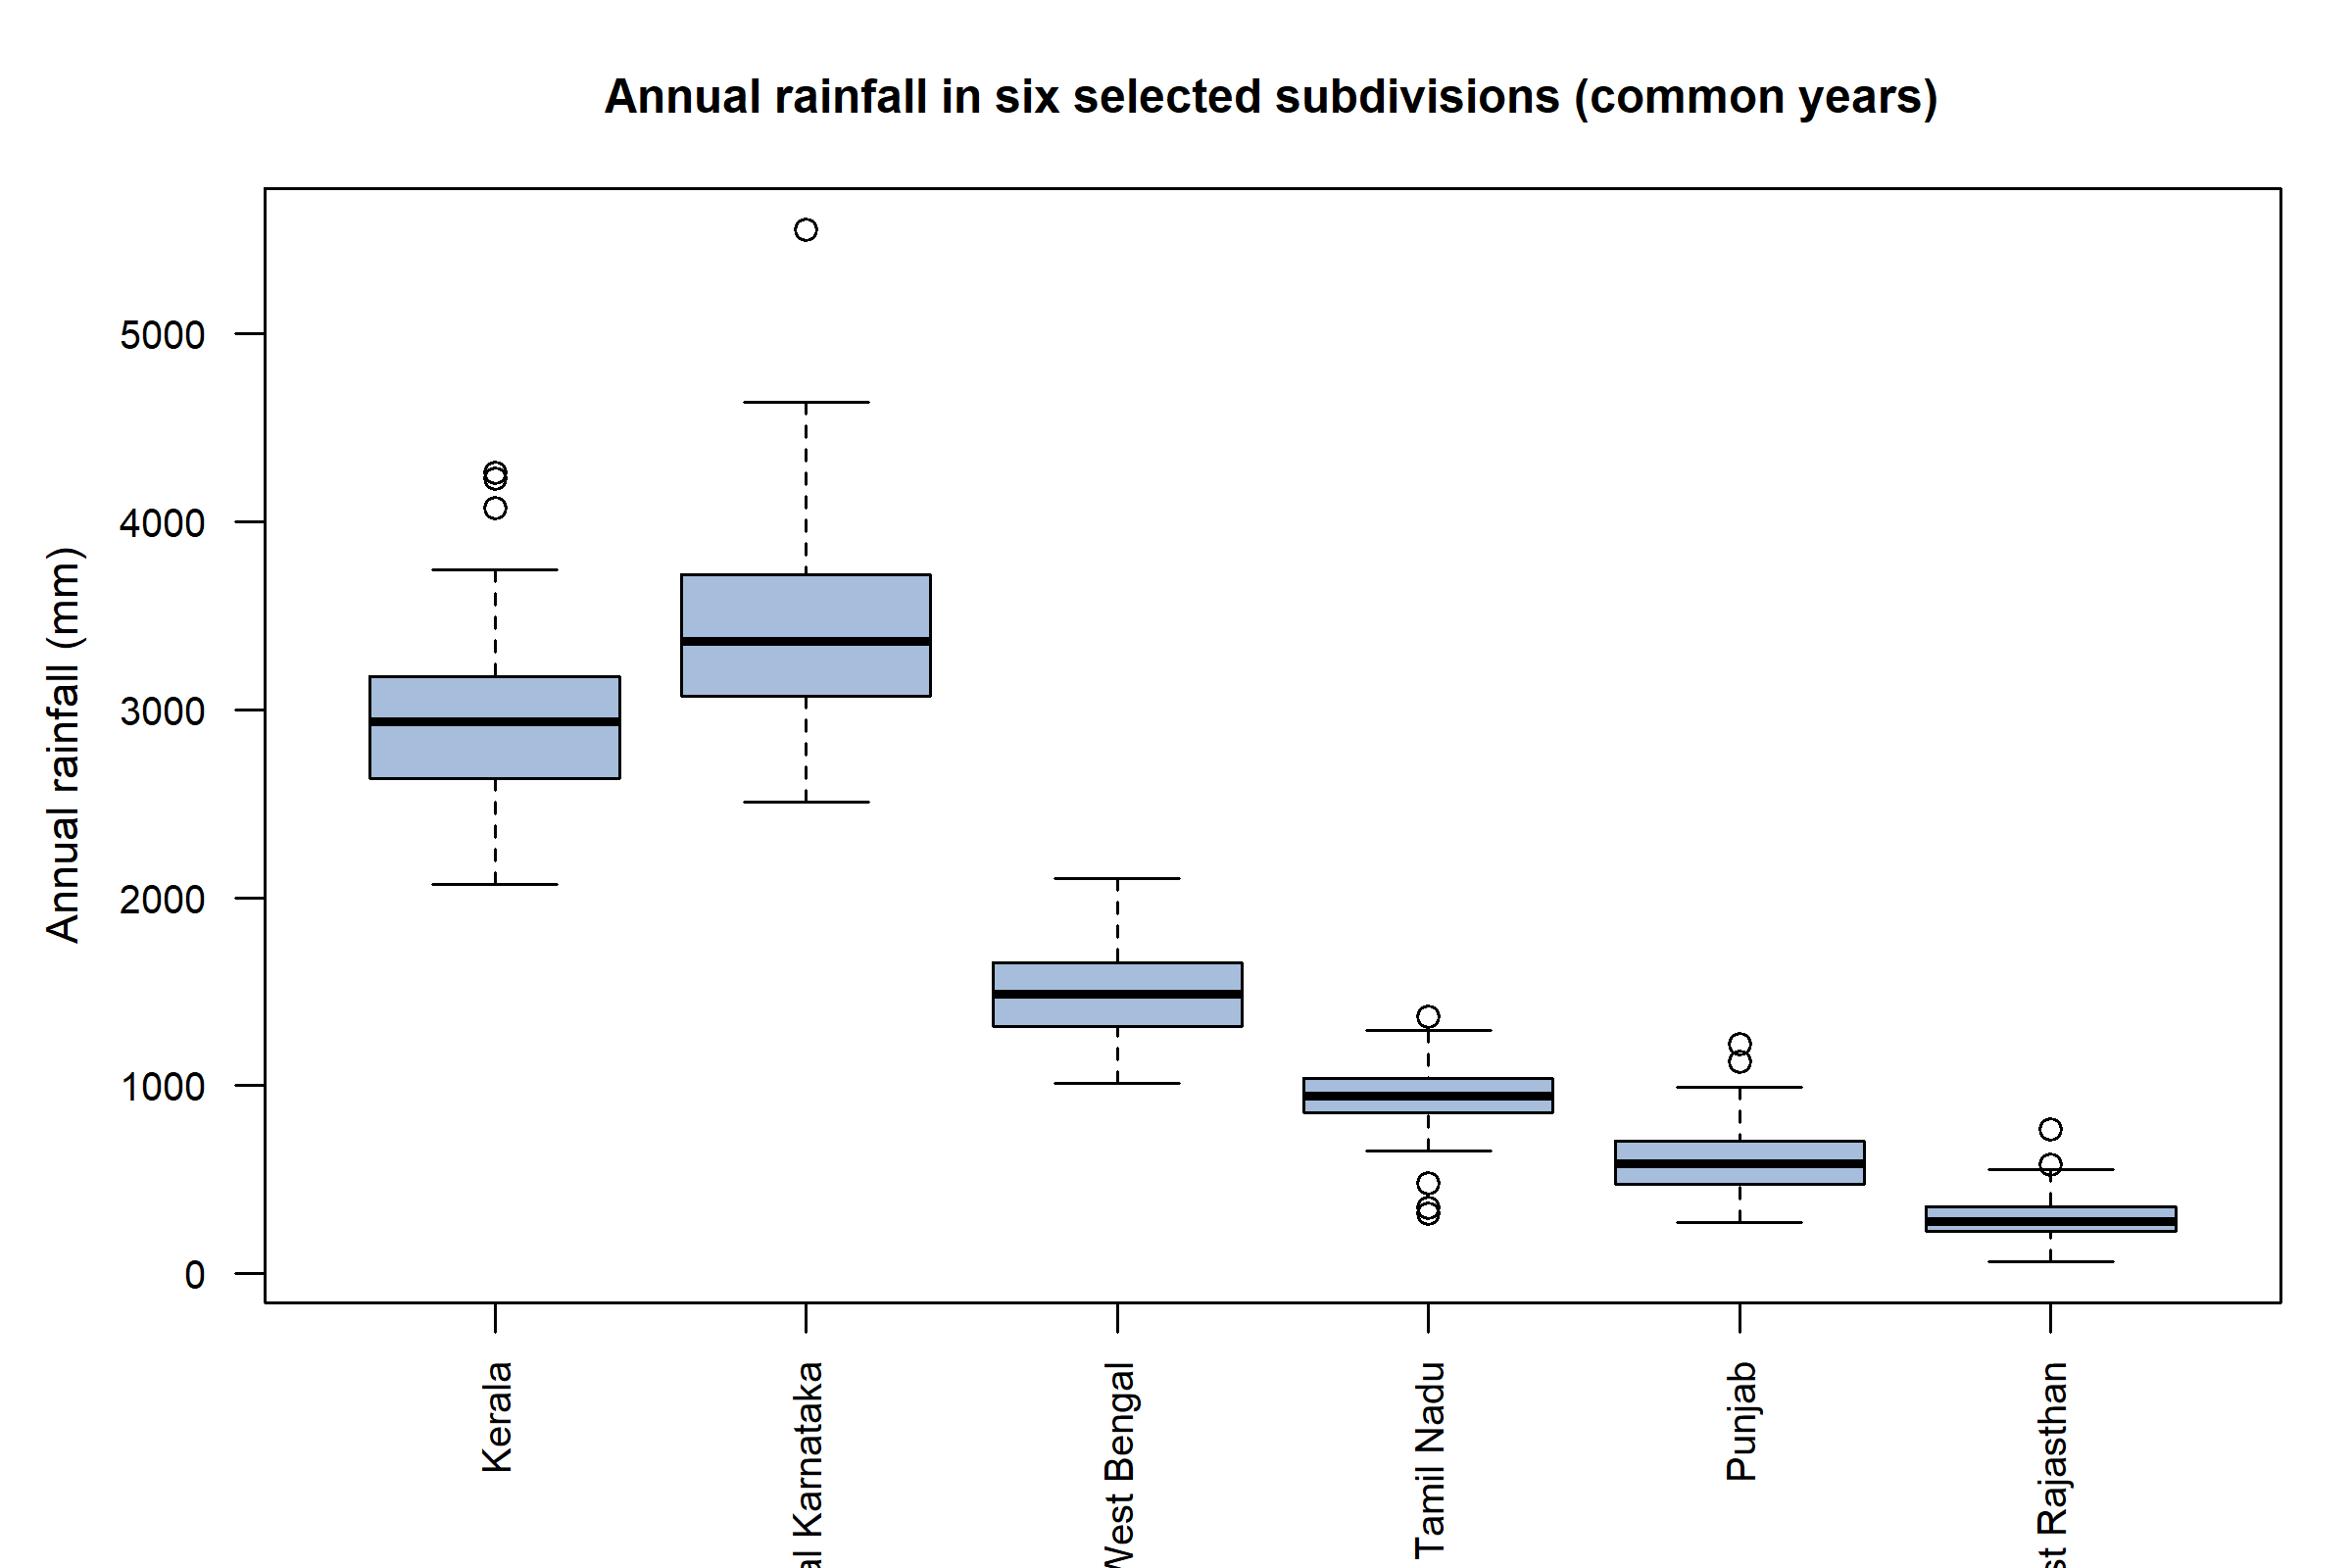
\includegraphics[width=0.92\linewidth]{../graphs/selected_regions_annual_boxplots} 

}

\caption{Figure 17. Annual rainfall (mm) in six selected subdivisions over common years. Spreads differ; Welch methods are appropriate.}\label{fig:fig-regbox}
\end{figure}

Figures 15--17 show both the mean gradient (Western Ghats and north-east
versus north-west India) and the CV gradient. West Rajasthan's high CV
(37.19\%) versus Kerala's (14.43\%) is why a single national CV of
9.36\% cannot describe every region.

\section{Time-series and trend
analysis}\label{time-series-and-trend-analysis}

\begin{figure}

{\centering 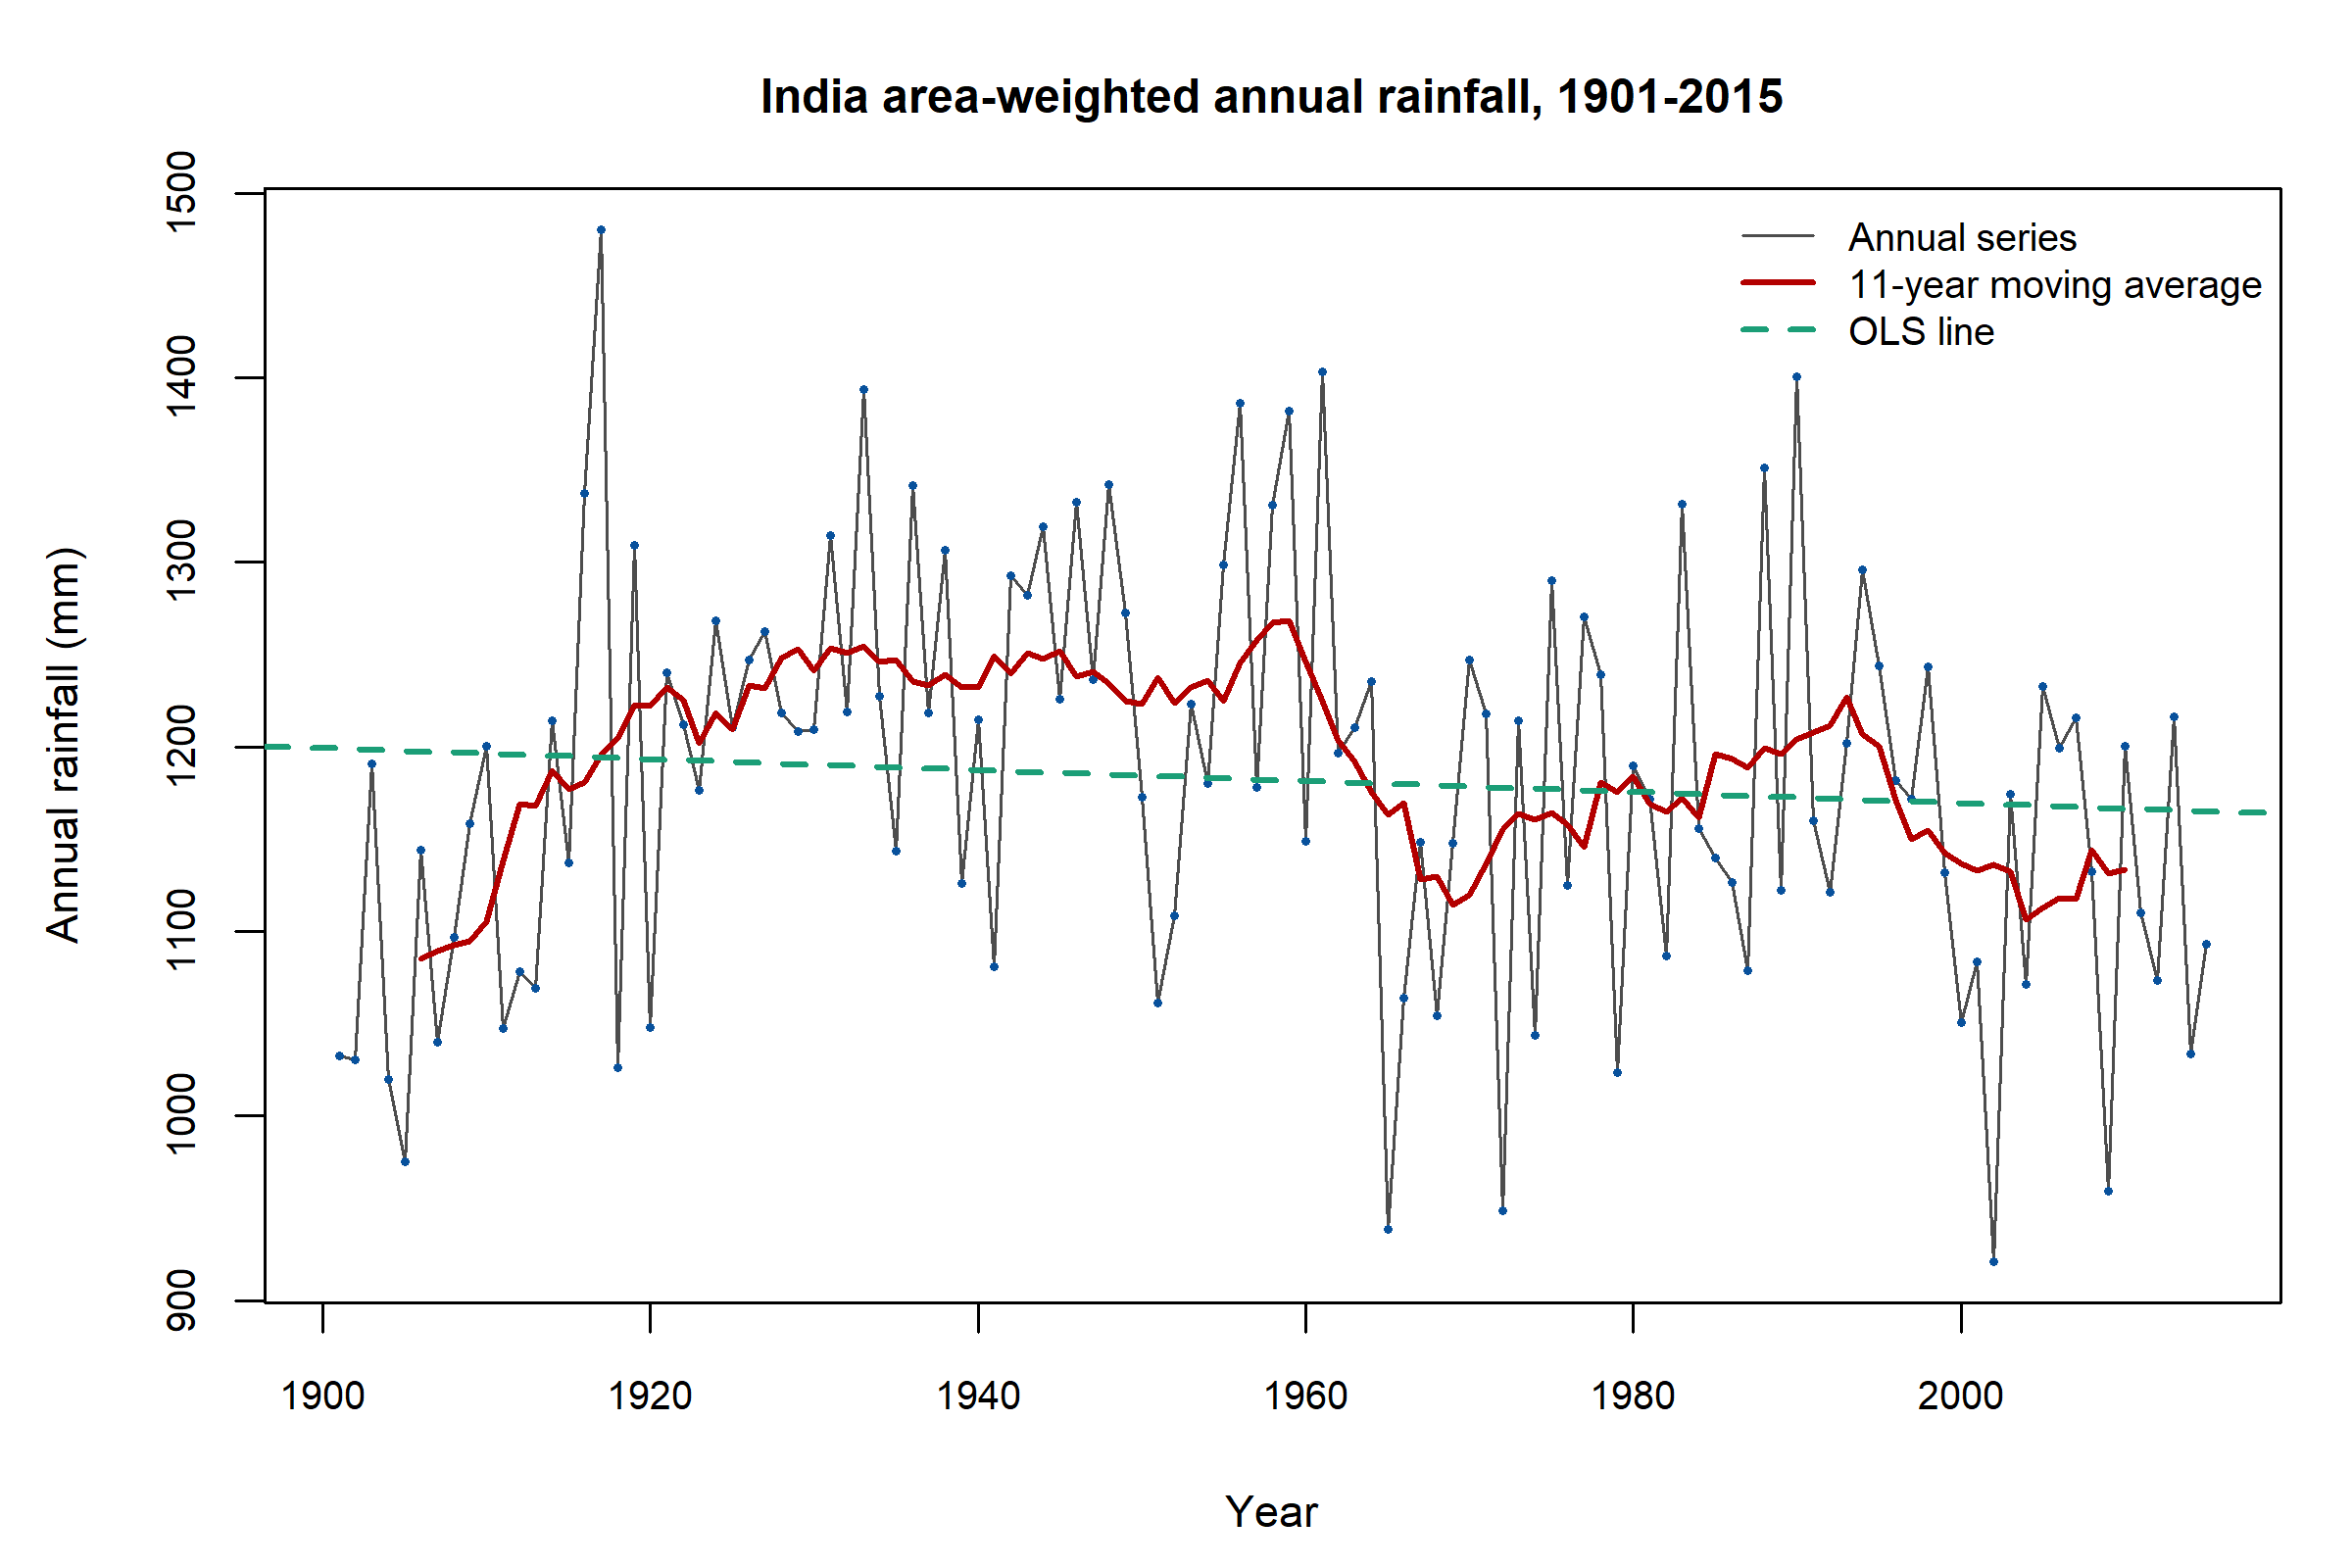
\includegraphics[width=0.92\linewidth]{../graphs/india_annual_timeseries} 

}

\caption{Figure 18. All-India annual rainfall (mm), 1901–2015, with an 11-year moving average and the OLS line. The smoother is descriptive; end years are missing because the window is incomplete.}\label{fig:fig-ts}
\end{figure}

\begin{figure}

{\centering 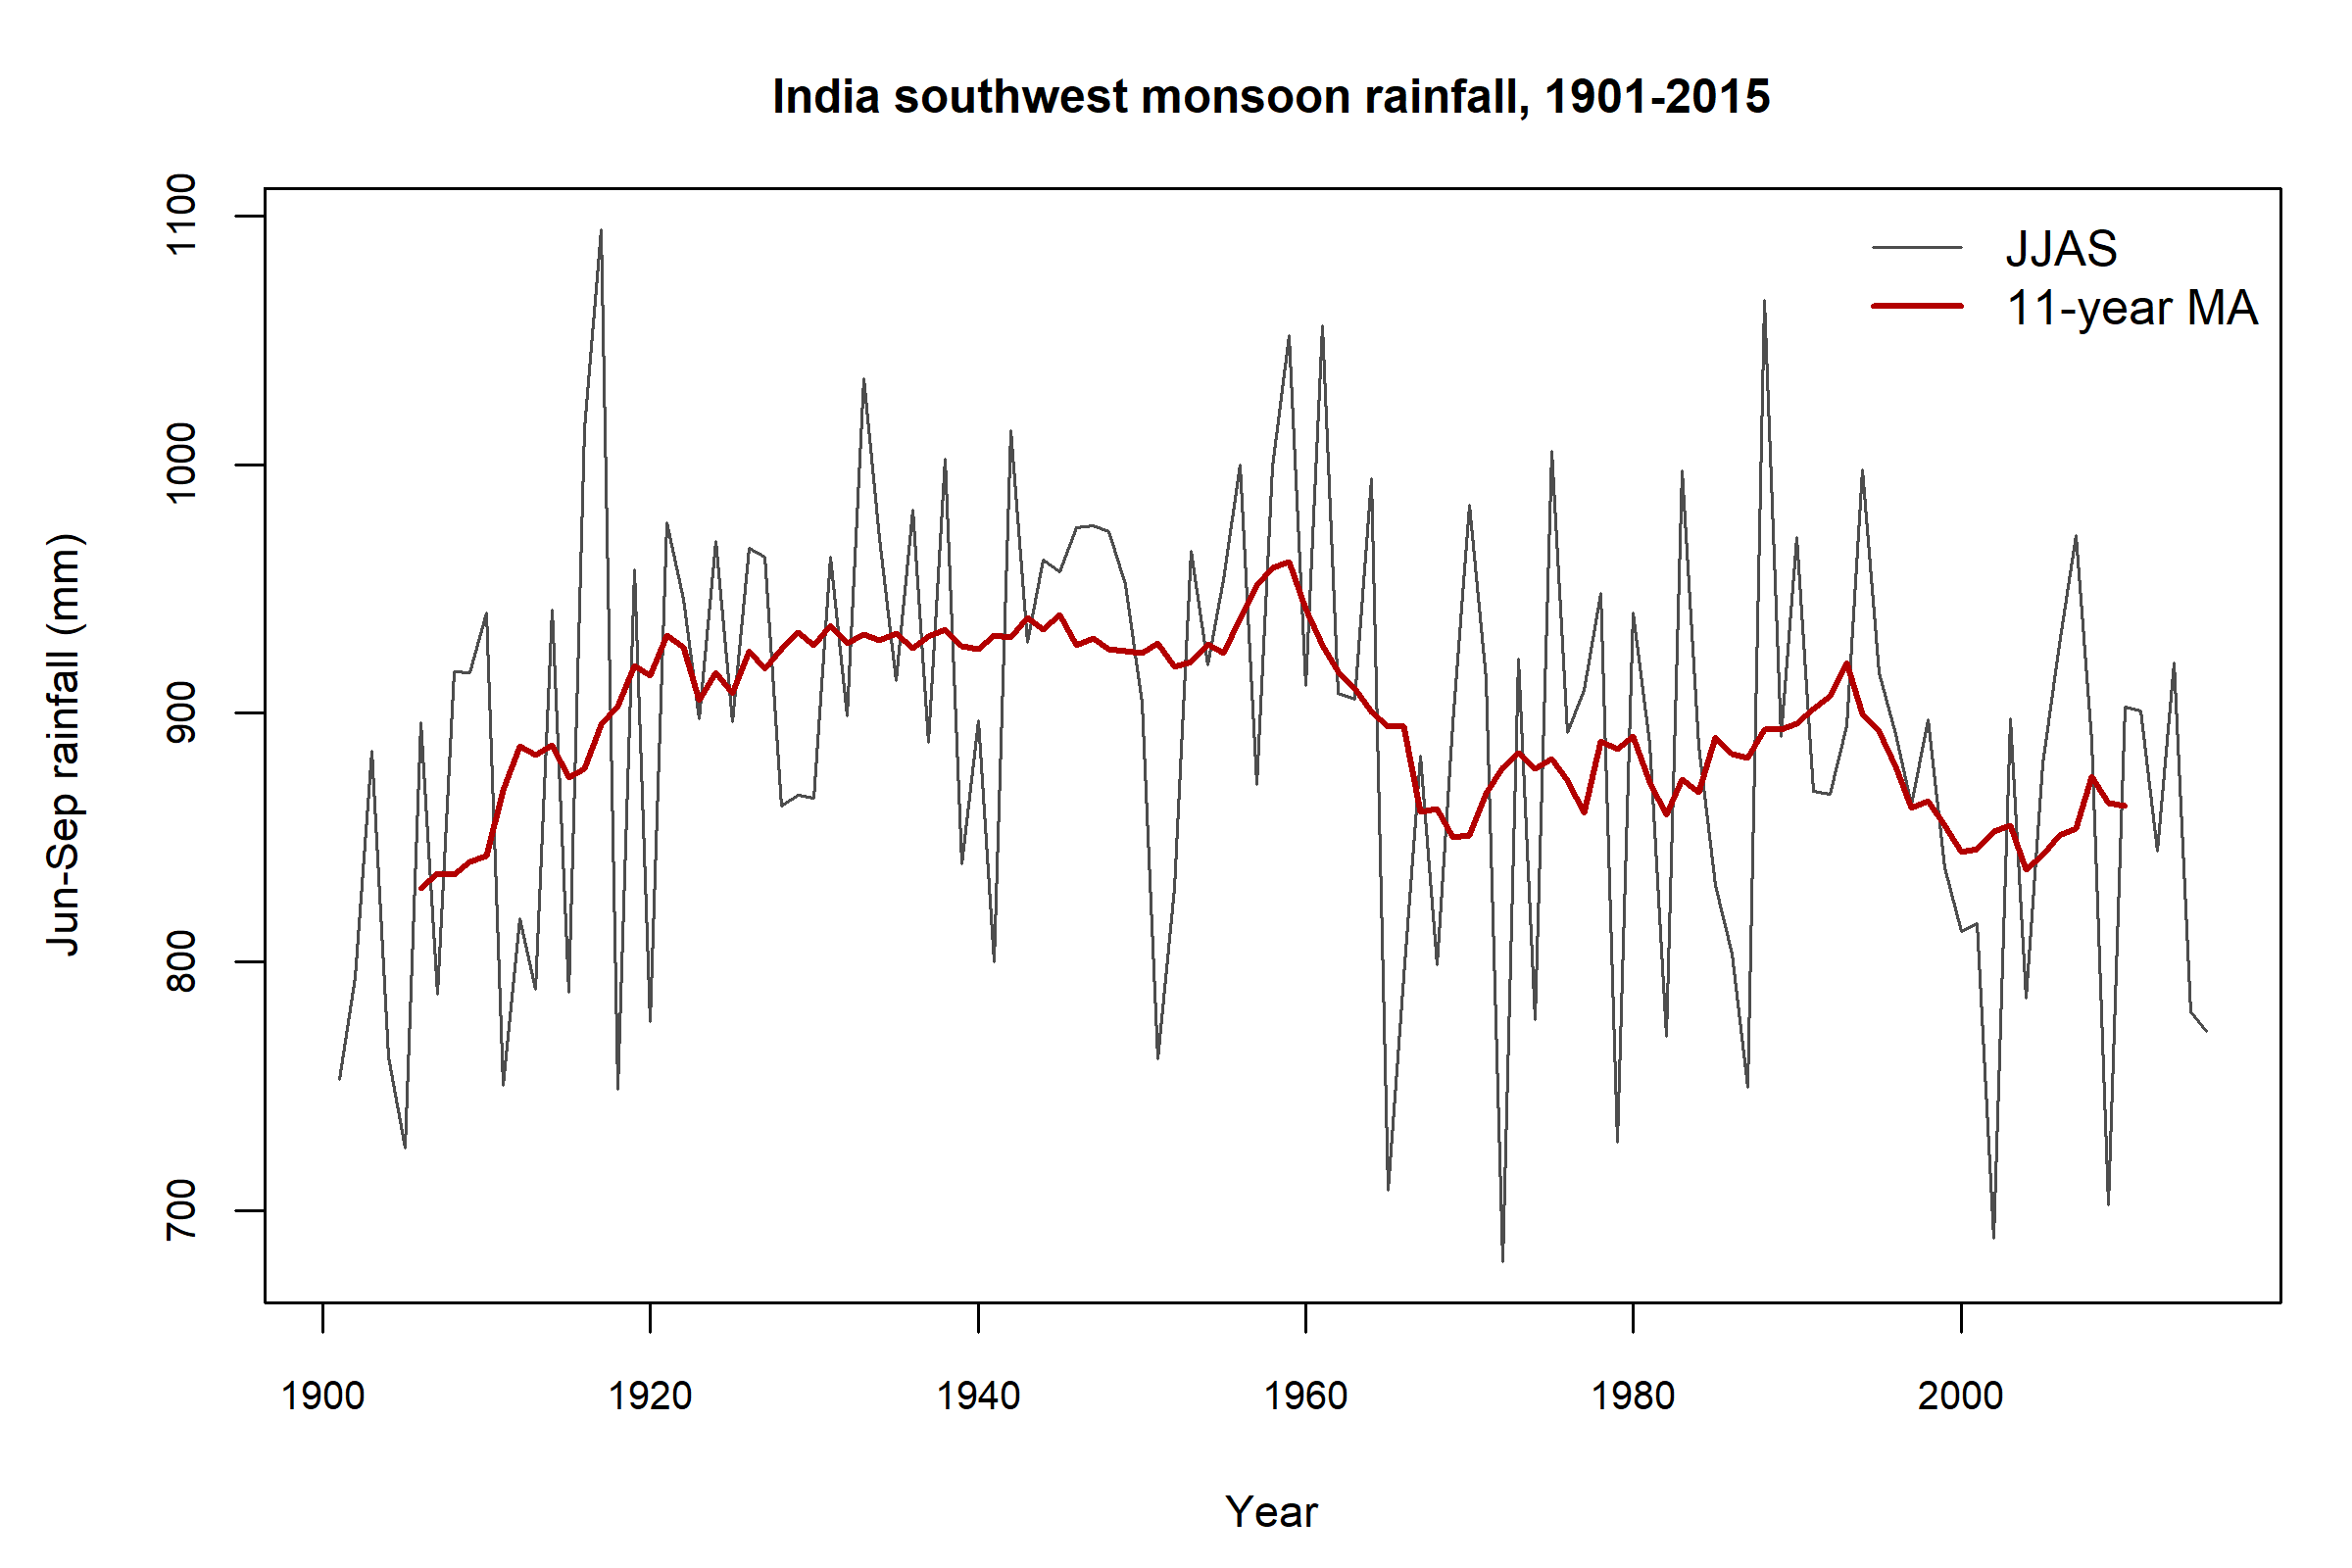
\includegraphics[width=0.92\linewidth]{../graphs/india_jjas_timeseries} 

}

\caption{Figure 19. All-India June–September rainfall (mm) and 11-year moving average, 1901–2015.}\label{fig:fig-jjas-ts}
\end{figure}

\begin{figure}

{\centering 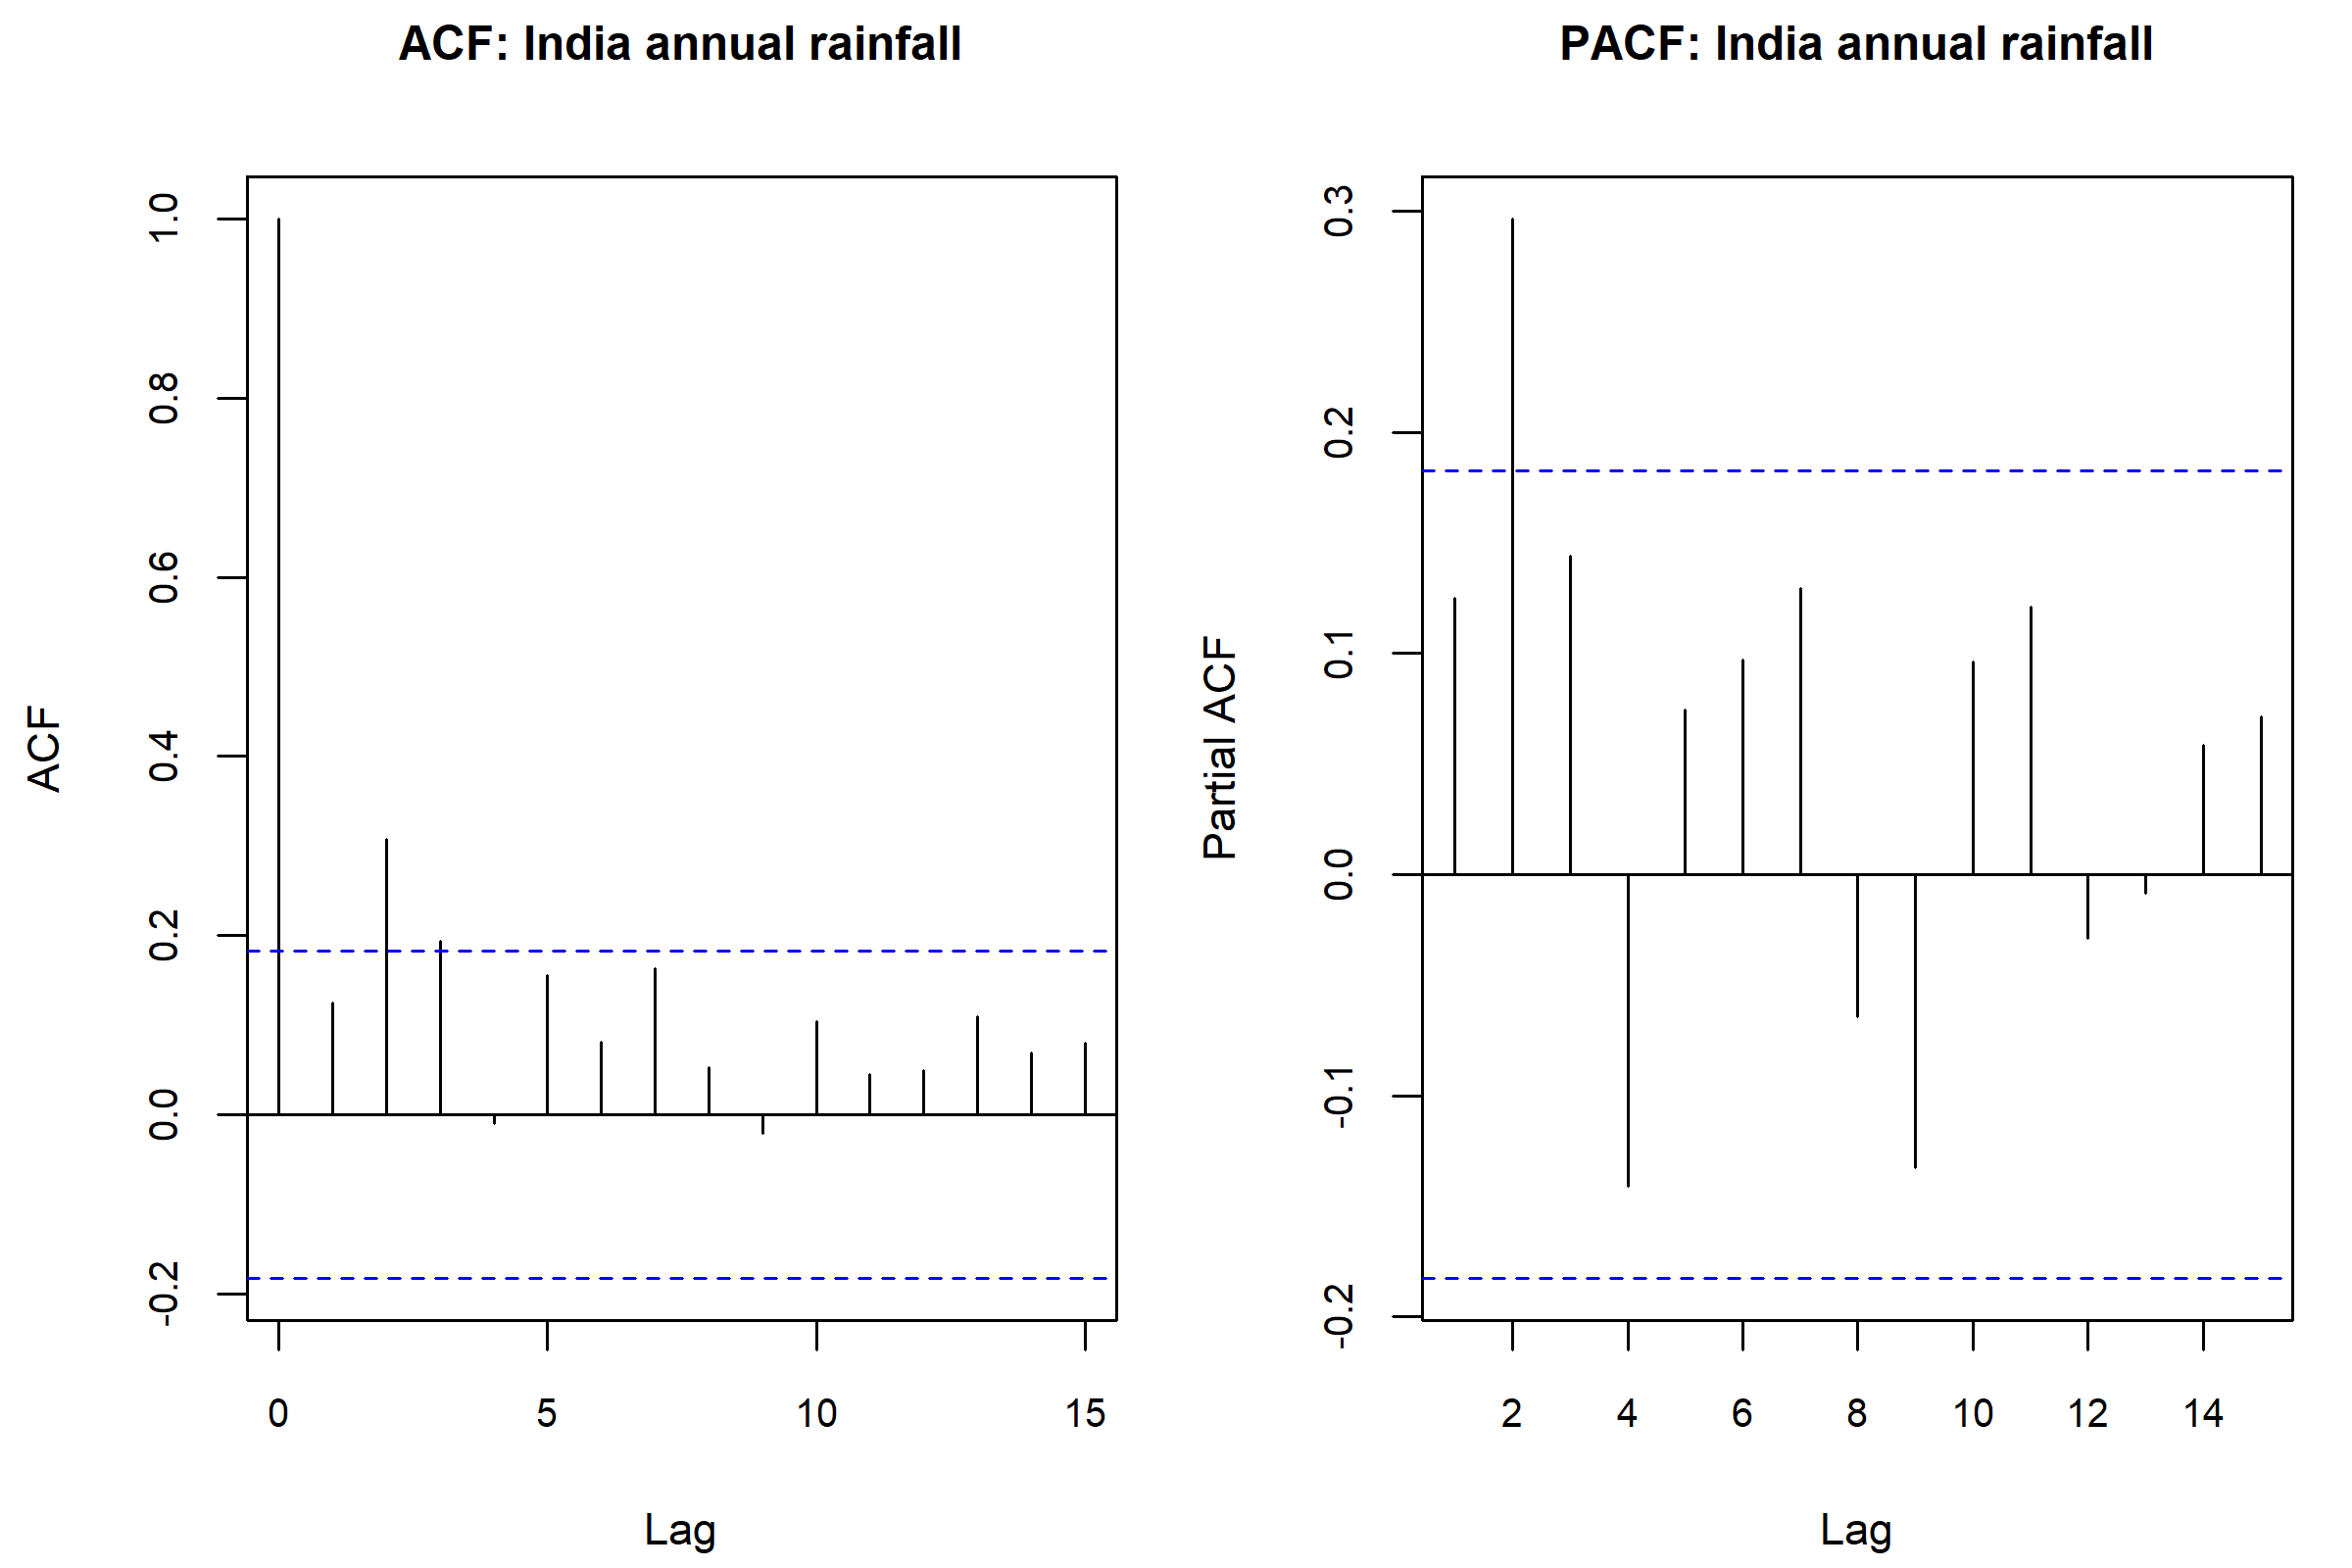
\includegraphics[width=0.92\linewidth]{../graphs/india_annual_acf} 

}

\caption{Figure 20. Sample ACF and PACF of all-India annual rainfall. The lag-2 autocorrelation exceeds the approximate white-noise bound.}\label{fig:fig-acf}
\end{figure}

The 11-year moving average is a smoother, not a test. Lag-1 sample ACF
of annual rainfall is 0.125 (inside the approximate
\(1.96/\sqrt{n}\approx 0.183\) bound). Lag-2 ACF is 0.308,
\textbf{outside} that bound, so years are not a pure white-noise series.
Mann--Kendall's simple variance formula is therefore an approximation; a
borderline \(p\)-value would not be treated as decisive.

\begin{longtable}[]{@{}
  >{\raggedright\arraybackslash}p{(\linewidth - 22\tabcolsep) * \real{0.0745}}
  >{\raggedleft\arraybackslash}p{(\linewidth - 22\tabcolsep) * \real{0.0213}}
  >{\raggedleft\arraybackslash}p{(\linewidth - 22\tabcolsep) * \real{0.1170}}
  >{\raggedleft\arraybackslash}p{(\linewidth - 22\tabcolsep) * \real{0.0638}}
  >{\raggedleft\arraybackslash}p{(\linewidth - 22\tabcolsep) * \real{0.1064}}
  >{\raggedleft\arraybackslash}p{(\linewidth - 22\tabcolsep) * \real{0.0798}}
  >{\raggedleft\arraybackslash}p{(\linewidth - 22\tabcolsep) * \real{0.0798}}
  >{\raggedleft\arraybackslash}p{(\linewidth - 22\tabcolsep) * \real{0.0904}}
  >{\raggedleft\arraybackslash}p{(\linewidth - 22\tabcolsep) * \real{0.0798}}
  >{\raggedleft\arraybackslash}p{(\linewidth - 22\tabcolsep) * \real{0.1170}}
  >{\raggedleft\arraybackslash}p{(\linewidth - 22\tabcolsep) * \real{0.0745}}
  >{\raggedleft\arraybackslash}p{(\linewidth - 22\tabcolsep) * \real{0.0957}}@{}}
\caption{Table 11. National trend summaries. Mann--Kendall and Sen's
slope are the preferred inferential summaries when OLS assumptions are
doubtful.}\tabularnewline
\toprule\noalign{}
\begin{minipage}[b]{\linewidth}\raggedright
series
\end{minipage} & \begin{minipage}[b]{\linewidth}\raggedleft
n
\end{minipage} & \begin{minipage}[b]{\linewidth}\raggedleft
ols\_slope\_mm\_per\_year
\end{minipage} & \begin{minipage}[b]{\linewidth}\raggedleft
ols\_slope\_p
\end{minipage} & \begin{minipage}[b]{\linewidth}\raggedleft
pearson\_r\_with\_year
\end{minipage} & \begin{minipage}[b]{\linewidth}\raggedleft
mann\_kendall\_S
\end{minipage} & \begin{minipage}[b]{\linewidth}\raggedleft
mann\_kendall\_Z
\end{minipage} & \begin{minipage}[b]{\linewidth}\raggedleft
mann\_kendall\_tau
\end{minipage} & \begin{minipage}[b]{\linewidth}\raggedleft
mann\_kendall\_p
\end{minipage} & \begin{minipage}[b]{\linewidth}\raggedleft
sen\_slope\_mm\_per\_year
\end{minipage} & \begin{minipage}[b]{\linewidth}\raggedleft
sen\_intercept
\end{minipage} & \begin{minipage}[b]{\linewidth}\raggedleft
durbin\_watson\_ols
\end{minipage} \\
\midrule\noalign{}
\endfirsthead
\toprule\noalign{}
\begin{minipage}[b]{\linewidth}\raggedright
series
\end{minipage} & \begin{minipage}[b]{\linewidth}\raggedleft
n
\end{minipage} & \begin{minipage}[b]{\linewidth}\raggedleft
ols\_slope\_mm\_per\_year
\end{minipage} & \begin{minipage}[b]{\linewidth}\raggedleft
ols\_slope\_p
\end{minipage} & \begin{minipage}[b]{\linewidth}\raggedleft
pearson\_r\_with\_year
\end{minipage} & \begin{minipage}[b]{\linewidth}\raggedleft
mann\_kendall\_S
\end{minipage} & \begin{minipage}[b]{\linewidth}\raggedleft
mann\_kendall\_Z
\end{minipage} & \begin{minipage}[b]{\linewidth}\raggedleft
mann\_kendall\_tau
\end{minipage} & \begin{minipage}[b]{\linewidth}\raggedleft
mann\_kendall\_p
\end{minipage} & \begin{minipage}[b]{\linewidth}\raggedleft
sen\_slope\_mm\_per\_year
\end{minipage} & \begin{minipage}[b]{\linewidth}\raggedleft
sen\_intercept
\end{minipage} & \begin{minipage}[b]{\linewidth}\raggedleft
durbin\_watson\_ols
\end{minipage} \\
\midrule\noalign{}
\endhead
\bottomrule\noalign{}
\endlastfoot
India annual & 115 & -0.2967 & 0.3423 & -0.089 & -357 & -0.861 & -0.054
& 0.3895 & -0.2722 & 1725.2 & 1.742 \\
India Jun-Sep & 115 & -0.2261 & 0.3692 & -0.085 & -418 & -1.008 & -0.064
& 0.3135 & -0.2536 & 1398.7 & 1.875 \\
\end{longtable}

\textbf{All-India annual.} OLS slope -0.2967 mm year\(^{-1}\), \(p=\)
0.3423. Mann--Kendall \(S=\) -357, \(\tau=\) -0.054, \(Z=\) -0.861,
\(p=\) 0.3895. Sen's slope -0.2722 mm year\(^{-1}\). \textbf{Do not
reject} ``no monotonic trend'' at 5\%.

\textbf{June--September.} Mann--Kendall \(p=\) 0.3135; Sen slope -0.2536
mm year\(^{-1}\). Same decision.

Selected regional Mann--Kendall tests (complete years) do \textbf{not}
all point the same way: Kerala \(\tau=\) -0.135, \(p=\) 0.0326 (negative
Sen slope); Coastal Karnataka \(p=\) 0.0027 (positive); Gangetic West
Bengal \(p=\) 0.0234 (positive); Tamil Nadu, Punjab and West Rajasthan
are not significant at 5\%. Mixed regional signs, plus multiple testing,
forbid a single ``India is drying/wetting'' slogan. None of these tests
identifies a cause.

\section{Results and discussion}\label{results-and-discussion}

Putting the pieces together:

\begin{enumerate}
\def\labelenumi{\arabic{enumi}.}
\tightlist
\item
  \textbf{Monsoon dominance is quantitative, not rhetorical.}
  June--September is about 75.3\% of mean annual rainfall and was the
  wettest IMD season in all 115 years.
\item
  \textbf{All-India annual rainfall is relatively stable year to year}
  (CV 9.36\%) and surprisingly close to a normal (and to a large-shape
  gamma) model. Local December rainfall in West Rajasthan is not: more
  than one-third of those months are dry zeros.
\item
  \textbf{Textbook 1180 mm} is compatible with this series mean (1182.03
  mm; 95\% CI 1161.59--1202.48 mm).
\item
  \textbf{Regions are not interchangeable.} Kerala minus West Rajasthan
  is about 2630 mm in mean annual rainfall; Welch and rank tests reject
  equality by an enormous margin. Relative variability is larger in arid
  subdivisions.
\item
  \textbf{Seasons of the same year are not independent groups}; pairing
  was used for monsoon versus post-monsoon. Winter and monsoon totals
  are only weakly and non-significantly correlated nationally.
\item
  \textbf{Deficient-monsoon years} are about 22\% of this record under a
  90\%-of-sample-mean rule. Early versus late period is not associated
  with that classification in a chi-square test (\(p=\) 0.8456).
\item
  \textbf{National trend tests are negative at 5\%.} OLS
  \(R^2\approx 0.008\); Mann--Kendall \(p=\) 0.3895. Some subdivisions
  show their own slopes; they do not add up to an attributed national
  climate signal.
\end{enumerate}

These findings are about \textbf{this IMD record}, under the assumptions
stated. They are suitable for a viva if the student can explain why
pairing, Welch, bootstrap KS, and Mann--Kendall were chosen.

\section{Limitations}\label{limitations}

\begin{itemize}
\tightlist
\item
  \textbf{One climate path.} The 115 years are not a simple random
  sample of hypothetical years.
\item
  \textbf{Temporal dependence.} Lag-2 autocorrelation of annual totals
  violates strict iid assumptions behind SEs, \(t\) intervals, OLS
  \(p\)-values and unmodified Mann--Kendall variance.
\item
  \textbf{LPA analogue.} Deficient/excess classes use this sample mean,
  not the official IMD LPA window.
\item
  \textbf{Unbalanced regional panel.} Missing years were not invented;
  ANOVA used a common complete-year window.
\item
  \textbf{National versus regional support.} Area-weighted India
  \(\neq\) mean of 36 boxes.
\item
  \textbf{No daily data.} Spell lengths, intensity and true waiting-time
  exponential models cannot be studied.
\item
  \textbf{IQR outlier flags.} Monthly rainfall is skewed, so many
  subdivision months are flagged; flags are not deletions.
\item
  \textbf{Multiple regional tests.} Six Mann--Kendall tests were not
  family-wise error controlled; significant regional slopes are
  exploratory.
\item
  \textbf{No causation.} Correlation, regression on year, and period
  \(\times\) category tables do not identify physical drivers.
\item
  \textbf{Exponential model} was never a serious candidate for annual
  totals; it is a teaching counter-example.
\item
  \textbf{Chi-square GOF} for wettest season has expected counts \(>5\)
  but observed zeros in three cells; the rejection is still obvious from
  the 115--0--0--0 table.
\end{itemize}

Analyses that were \textbf{not} done, because they would not be
justified: chi-square tests on raw millimetres; independent \(t\)-tests
of two seasons from the same year; correlating annual totals with
June--September; deleting extremes to ``clean'' monsoon; imputing
missing monthly rain; claiming proof of climate change.

\section{Conclusion}\label{conclusion}

Official IMD millimetre records, cleaned without fabrication, show an
all-India climate whose annual total averages about 1182.03 mm, is
dominated by June--September, and is compatible with a 1180 mm
benchmark. Probability models that respect positivity (gamma) and models
that do not (normal) both describe the \emph{national annual} series
reasonably; exponential does not. Regional India is another story: means
and CVs differ by an order of magnitude, and Welch ANOVA rejects a
common mean among six representative subdivisions. National linear and
Mann--Kendall trends over 1901--2015 are not significant at 5\%. The
honest statistical conclusion is descriptive and comparative, not
causal.

\section{References}\label{references}

\begin{enumerate}
\def\labelenumi{\arabic{enumi}.}
\tightlist
\item
  India Meteorological Department (IMD), Ministry of Earth Sciences,
  Government of India. Area-weighted monthly, seasonal and annual
  rainfall series for India, 1901--2015. Data file:
  \texttt{rainfall\_area-wt\_India\_1901-2015.csv}.
\item
  India Meteorological Department (IMD), Ministry of Earth Sciences,
  Government of India. Rainfall for meteorological sub-divisions of
  India, records through 2017. Data file:
  \texttt{Sub\_Division\_IMD\_2017.csv}.
\item
  India Meteorological Department. Operational practice of classifying
  southwest monsoon seasonal rainfall as deficient, normal or excess
  relative to a long-period average (LPA). This project uses 90\% and
  110\% of the \emph{sample} mean as an analogue, not a substitute for
  the official LPA.
\item
  Wilcoxon, F. (1945). Individual comparisons by ranking methods.
  \emph{Biometrics Bulletin}, 1(6), 80--83.
\item
  Mann, H. B. (1945). Nonparametric tests against trend.
  \emph{Econometrica}, 13(3), 245--259.
\item
  Kendall, M. G. (1975). \emph{Rank Correlation Methods}. Charles
  Griffin.
\item
  Sen, P. K. (1968). Estimates of the regression coefficient based on
  Kendall's tau. \emph{Journal of the American Statistical Association},
  63(324), 1379--1389.
\item
  Shapiro, S. S., and Wilk, M. B. (1965). An analysis of variance test
  for normality. \emph{Biometrika}, 52(3--4), 591--611.
\item
  Lilliefors, H. W. (1967). On the Kolmogorov--Smirnov test for
  normality with mean and variance unknown. \emph{Journal of the
  American Statistical Association}, 62(318), 399--402.
\item
  Welch, B. L. (1947). The generalization of `Student's' problem when
  several different population variances are involved.
  \emph{Biometrika}, 34(1--2), 28--35.
\item
  Durbin, J., and Watson, G. S. (1950). Testing for serial correlation
  in least squares regression. I. \emph{Biometrika}, 37(3--4), 409--428.
\item
  Cook, R. D. (1977). Detection of influential observation in linear
  regression. \emph{Technometrics}, 19(1), 15--18.
\item
  Wilks, D. S. (2011). \emph{Statistical Methods in the Atmospheric
  Sciences} (3rd ed.). Academic Press.
\item
  Helsel, D. R., and Hirsch, R. M. (2002). \emph{Statistical Methods in
  Water Resources}. U.S. Geological Survey.
\item
  R Core Team (2026). \emph{R: A Language and Environment for
  Statistical Computing}. R Foundation, Vienna. Version 4.6.1.
\end{enumerate}

\section{Appendix}\label{appendix}

\subsection{A. Project layout and how to
rerun}\label{a.-project-layout-and-how-to-rerun}

From the folder that contains \texttt{data/} and \texttt{R\_code/}, in
RStudio:

\begin{Shaded}
\begin{Highlighting}[]
\FunctionTok{source}\NormalTok{(}\StringTok{"R\_code/01\_data\_inspection.R"}\NormalTok{)}
\FunctionTok{source}\NormalTok{(}\StringTok{"R\_code/02\_data\_cleaning.R"}\NormalTok{)}
\FunctionTok{source}\NormalTok{(}\StringTok{"R\_code/10\_run\_phase2.R"}\NormalTok{)}
\FunctionTok{source}\NormalTok{(}\StringTok{"R\_code/11\_render\_report.R"}\NormalTok{)}
\end{Highlighting}
\end{Shaded}

Scripts \texttt{03}--\texttt{09} produce tables and figures; \texttt{11}
knits this file to Word (and PDF if LaTeX is installed). Relative paths
are used throughout.

\subsection{B. Concept coverage}\label{b.-concept-coverage}

See \texttt{results/tables/concept\_coverage\_matrix.csv} for the
mapping from statistical technique to script, table, figure and report
section.

\subsection{C. Selected implementation
notes}\label{c.-selected-implementation-notes}

\begin{itemize}
\tightlist
\item
  Gamma MLE uses \texttt{nlm} on the negative log-likelihood, started at
  method-of-moments estimates.
\item
  Bootstrap KS re-fits the candidate law on each simulated sample of
  size \(n\) and compares the KS statistic to the observed statistic.
\item
  Mann--Kendall and Sen's slope are implemented in
  \texttt{R\_code/00\_project\_helpers.R} (base R; no extra packages).
\item
  Cleaning never overwrites \texttt{data/}.
\end{itemize}

\subsection{D. Additional output
files}\label{d.-additional-output-files}

Hypothesis write-ups:
\texttt{results/statistical\_outputs/hypothesis\_testing\_report.txt}.\\
Distribution notes:
\texttt{results/statistical\_outputs/distribution\_fit\_notes.txt}.\\
Trend notes:
\texttt{results/statistical\_outputs/time\_series\_trend\_notes.txt}.\\
Regional notes:
\texttt{results/statistical\_outputs/regional\_anova\_notes.txt}.

The appendix does not reprint entire scripts; faculty can open
\texttt{R\_code/} in RStudio. Student name, roll number and a signed
originality statement should be added on the title page before binding.

\end{document}
